\begin{figure}
\centering
\pandocbounded{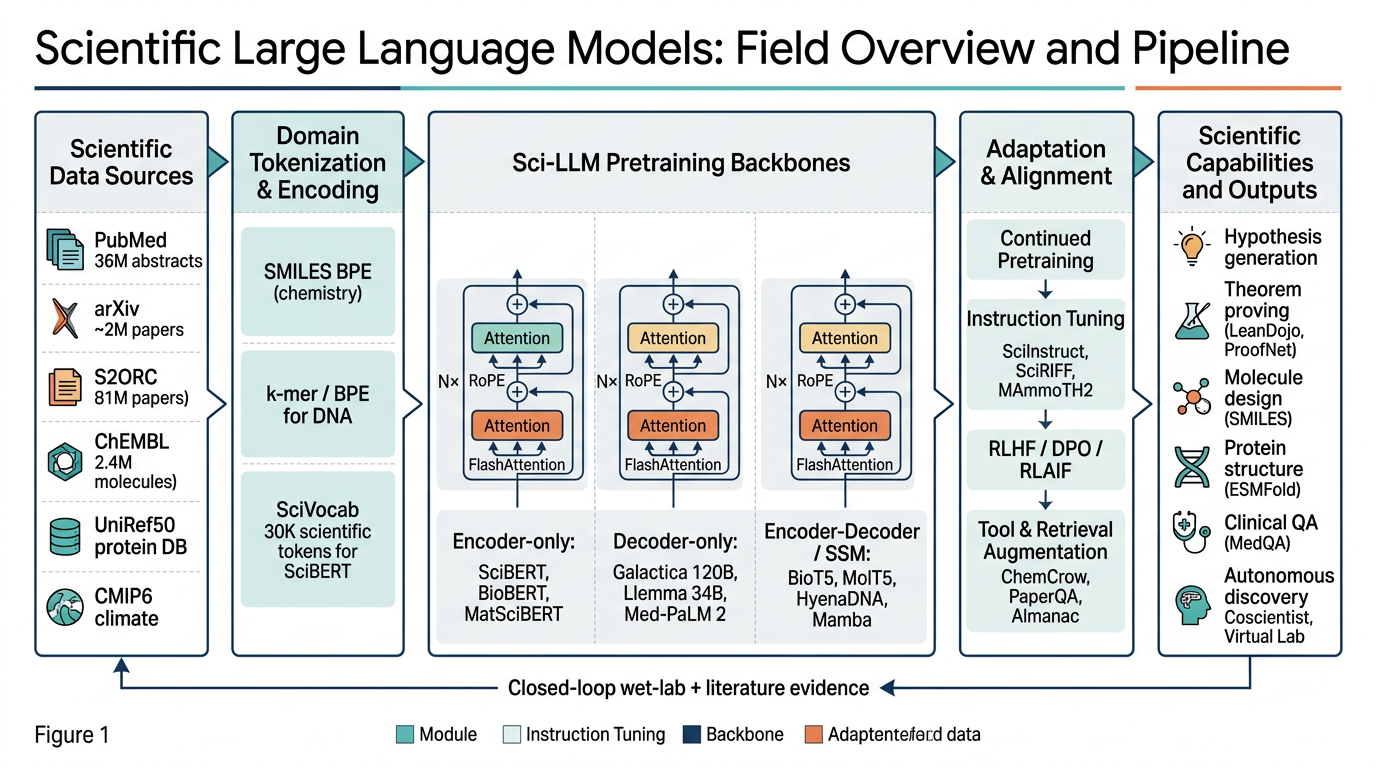
\includegraphics[keepaspectratio,alt={Field overview and pipeline of Scientific Large Language Models, from data sources through tokenization, pretraining, alignment, and capabilities.}]{./figures/Scientific-Large-Language-Models__fig1_overview.png}}
\caption{Field overview and pipeline of Scientific Large Language Models, from data sources through tokenization, pretraining, alignment, and capabilities.}
\end{figure}

\section{Executive Overview}\label{executive-overview}

The historical arc surveyed in §2 partitions into three sharp inflections. The encoder era of 2018--2021 was opened by SciBERT {[}15{]} and BioBERT {[}14{]} on PubMed and S2ORC. The decoder and scaling era of 2022--2024 was triggered by Galactica's 120B-parameter, 106B-token release {[}1{]}, by Med-PaLM and Med-PaLM 2 reaching 67.6\% then 86.5\% MedQA {[}11, 18{]}, by ESM-2 at 15B parameters with 60×-faster ESMFold {[}25{]}, by Coscientist's autonomous Pd cross-coupling {[}8{]}, and by ChemCrow's 18-tool agent {[}12{]}. The agentic and reasoning-tuned era of 2025--2026 is defined by reasoning-RL post-training in o1, DeepSeek-R1 (671B MoE), QwQ, and Gemini-Thinking, and by multi-agent stacks such as Virtual Lab {[}19{]} and Agent Laboratory {[}20{]}.

Methodologically, §§4--7 span SciVocab and BPE or k-mer tokenization, the citation tokens \texttt{{[}\$START\_R\$EF{]}...{[}\$END\_R\$EF{]}} and working-memory tokens \texttt{\textless{}work\textgreater{}} introduced by Galactica, continued pretraining at 1e-5 learning rate over 1--3 epochs in Llemma, BioMistral, and GeoGalactica, instruction tuning on SciInstruct (200K), SciRIFF (137K instructions across 54 tasks), and MAmmoTH2 (10M), preference alignment via PPO, DPO, and RLAIF, retrieval-augmented generation in PaperQA and Almanac, tool-augmented ReAct loops in ChemCrow and Coscientist, and reasoning RL on chain-of-thought traces.

The benchmark landscape catalogued in §9 has shifted as MedQA, MMLU-STEM, and GSM8K saturate. Attention now centres on GPQA-Diamond (198 graduate questions; o1-class ≈78\%), OlympicArena (11,163 problems; GPT-4o 39.97\%), SciBench (789 problems; GPT-4 35.8\%), MicroVQA (1,042 microscopy questions; GPT-4o 53.5\%), LLM-SRBench equation discovery (\textless40\%), ChemPro (4,100 progressive questions), GUE (28 DNA tasks), miniF2F, ProofNet (371 Lean problems), and the long-form factuality scorer SAFE.

The limitations dissected in §10 include hallucinated citations (canonically illustrated by Galactica's three-day retraction), 20--40\% missed differential diagnoses on real clinical cases {[}60{]}, dual-use synthesis risks {[}59{]}, retrieval drift, plan-step explosion (where 0.95\^{}20 ≈ 0.36 success caps long-horizon agents), calibration drift after RLHF, and benchmark contamination. The standard mitigations are RAG over curated corpora (Almanac: 91\% vs 64\% factuality versus ChatGPT), tool-level safety filters such as ChemCrow's SMARTS checks, conformal prediction, and post-cutoff held-out evaluation.

The predictions developed in §12 take the form of five falsifiable forecasts for 2027--2028: (F1) an agentic Sci-LLM as primary contributor on a top-venue paper; (F2) ESM descendants delivering functional binders without de-novo MSAs in at least half of attempts; (F3) FDA clearance of medical Sci-LLMs in three narrow domains; (F4) curated and citation-verified scientific corpora of at least 500B tokens as the default pretraining base; and (F5) the open-weights to closed-API gap on GPQA-Diamond closing to within 5 absolute points.

Sections §§1--2 fix terminology and history; §3 fixes the taxonomy; §§4--5 cover algorithmic mechanism and alignment; §§6--7 cover augmentation and agentic autonomy; §8 walks each domain; §9 catalogues data and benchmarks; §10 dissects failure modes; §11 audits compute and reproducibility; §12 fixes the open-problem agenda; and §13 is the glossary and reference map.

\section{Concept and Scope of Scientific Large Language Models}\label{concept-and-scope-of-scientific-large-language-models}

A Sci-LLM is a transformer-based foundation model whose pretraining corpus, vocabulary, and downstream evaluation are explicitly anchored to the language of science. That language includes scientific prose, mathematical notation, programming code for simulation and analysis, and structured biochemical strings such as SMILES, FASTA, IUPAC names, and Lean tactics. The term gained currency after Galactica (Taylor et al., November 2022) {[}1{]}, the first decoder-only model trained at 120B parameters almost exclusively on a curated 106B-token scientific corpus. A coordinated 2024--2026 wave of surveys then crystallized the term: Zhang et al.~in \emph{ACM Computing Surveys} {[}2{]}, the cross-discipline survey of Zhang, Chen, Jin et al.~{[}3{]}, \emph{LLM4SR} {[}4{]}, and \emph{From AI for Science to Agentic Science} {[}5{]}. The community now uses \textbf{Sci-LLM} for any foundation model whose primary inductive bias is the distribution of scientific artifacts. General-purpose LLMs, by contrast, target broad web text.

A Sci-LLM differs from a general LLM along three operational axes. First, \textbf{input modality}: Sci-LLMs ingest symbolic systems with different statistical regularities alongside natural-language tokens. Examples include SMILES, where parentheses encode branching and a one-character change alters the molecule; FASTA, a 20-letter amino-acid alphabet with context spanning hundreds of residues; and macro-rich LaTeX. Second, \textbf{output validity}: a Sci-LLM is judged not only on fluency but on whether its output parses, balances atoms, type-checks in Lean, or matches an experimentally measured value. Galactica introduced explicit \emph{citation tokens} \texttt{{[}\$START\_R\$EF{]}...{[}\$END\_R\$EF{]}} and \emph{working-memory tokens} \texttt{\textless{}work\textgreater{}} so that intermediate steps and references became first-class training targets {[}1{]}. Third, \textbf{grounding requirement}: Sci-LLMs are typically deployed alongside literature retrieval (PaperQA {[}6{]}, Almanac {[}7{]}), simulators, or wet-lab automation. Boiko et al.'s Coscientist (\emph{Nature} 2023) {[}8{]} couples a GPT-4 reasoning module with planning, execution, and an OPENTRONS robot for Pd-catalysed cross-coupling. The LLM is one component of a closed scientific loop rather than a stand-alone oracle.

Formally, a Sci-LLM defines a distribution \(p_\theta(Y \mid X)\) over scientific outputs \(Y\) given context \(X\). Inputs \(X\) may be a research question, an EHR note, a partial molecule, or a DNA window; outputs \(Y\) may be a cited free-text answer, a SMILES string, a multi-step derivation, or a robot action plan. Pretraining minimizes \(\mathcal{L}_{\text{pre}}(\theta) = -\mathbb{E}_{x \sim D_{\text{sci}}}\big[\sum_t \log p_\theta(x_t \mid x_{<t})\big]\) over a scientific corpus \(D_{\text{sci}}\). Adaptation then proceeds via continued pretraining, supervised instruction tuning on corpora such as \textbf{SciInstruct} (200K self-reflective examples) {[}9{]} or \textbf{SciRIFF} (137K instructions across 54 tasks) {[}10{]}, RLHF as in \textbf{Med-PaLM 2} {[}11{]}, or tool/retrieval augmentation as in \textbf{ChemCrow} {[}12{]}. The literature now treats \emph{grounding} and \emph{verification} as first-class evaluation axes; Guo et al.'s \emph{PNAS} 2026 high-Tc superconductivity case study probes whether LLMs encode valid \emph{world models} of materials rather than surface-level fluency {[}13{]}.

Sci-LLMs span a four-tier \textbf{scientific reasoning hierarchy}. At the base lies factual recall, the regime of BioBERT {[}14{]} and SciBERT {[}15{]} for biomedical Named Entity Recognition (NER), concept linking, and relation extraction. One tier up sits symbolic manipulation. Llemma 34B {[}16{]} and Minerva continue equations, and LeanDojo augments theorem proving with retrieval over 98K Lean theorems {[}17{]}. The third tier is multi-step deduction. Chain-of-thought-trained Med-PaLM 2 reaches 86.5\% on MedQA, up from the 67.6\% Med-PaLM baseline {[}11, 18{]}. The apex is hypothesis generation and experimental planning. Swanson et al.'s Virtual Lab designed novel SARS-CoV-2 nanobodies that were experimentally validated against KP.3 and JN.1 variants {[}19{]}. Schmidgall et al.'s Agent Laboratory wraps literature-review, planning, execution, and report-writing into a single agentic loop {[}20{]}. Zheng et al.'s 2025 survey \emph{From Automation to Autonomy} {[}21{]} argues that the field's trajectory is the climb up this ladder.

A core conceptual claim, revisited in §10, is that a Sci-LLM is not merely a generic LLM evaluated on science questions. Its pretraining distribution, tokenization, alignment data, evaluation metrics, and runtime tool stack are jointly reshaped by scientific desiderata. SciBERT, for example, introduced \textbf{SciVocab}, a 30K-token WordPiece vocabulary learned on 1.14M Semantic Scholar papers (18\% biomedical, 82\% mixed sciences). SciVocab lifted single-token coverage of biomedical entities by 42\% over BERT-base's WikiVocab {[}15{]}. MatSciBERT extended the idea to materials with ≈1M abstracts and gained +6 F1 on materials NER {[}22{]}. DNABERT used overlapping k-mer tokenization (k = 3, 4, 5, 6). DNABERT-2 replaced k-mers with byte-pair encoding (BPE), cutting parameters by ≈28\% while improving multispecies generalization across the 28-task GUE benchmark {[}23, 24{]}. These differences are not cosmetic. Token granularity propagates into context length, scaling laws, and downstream calibration.

The category overlaps with --- but is not identical to --- \textbf{biological sequence foundation models}. The ESM-2 family scales to 15B parameters on UniRef50's ≈65M protein clusters and outputs per-residue and pairwise embeddings; coupled with ESMFold, it predicts atomic-level structure ≈60× faster than AlphaFold 2 on single chains while remaining competitive in accuracy {[}25{]}. Whether ESM-2 is a ``Sci-LLM'' or a ``protein language model'' is partly terminological. The 2025 ACM CSUR survey {[}2{]} adopts the inclusive position that any large transformer trained on scientific tokens --- English text, SMILES, or amino acids --- counts; we follow that convention. By the same criterion the Nucleotide Transformer (2.5B parameters, 850 species; \emph{Nature Methods} 2024) {[}26{]}, HyenaDNA (1-million-base-pair context) {[}27{]}, and Enformer (gene-expression prediction) {[}28{]} are all Sci-LLMs specialised to genomic language.

A final conceptual boundary concerns \textbf{what is not a Sci-LLM}. Single-task supervised models such as Foldseek for structural search {[}Foldseek{]}, or Enformer when used purely as a deterministic regressor without language-style generation, are treated as adjacent rather than central. Vision--language models such as Flamingo {[}Flamingo{]} or consumer Gemini variants qualify only when trained or instruction-tuned jointly on scientific imagery and language --- Med-Gemini {[}29{]} qualifies; consumer GPT-4V chat does not. We adopt the inclusion threshold of Hu et al.~(2025) {[}30{]}: a model is a Sci-LLM if at least one training stage is dominated by scientific data, \textbf{or} if its primary deployment loop runs in a scientific environment.

Table 1.1 fixes the symbols and notation used throughout the survey, aligned with the conventions of the recent Sci-LLM surveys {[}2, 3, 4, 5, 21, 30{]} and the \emph{Survey on LLMs in Biology and Chemistry} {[}31{]}.

{\def\LTcaptype{none} % do not increment counter
\begin{longtable}[]{@{}
  >{\raggedright\arraybackslash}p{(\linewidth - 2\tabcolsep) * \real{0.4551}}
  >{\raggedright\arraybackslash}p{(\linewidth - 2\tabcolsep) * \real{0.5449}}@{}}
\toprule\noalign{}
\begin{minipage}[b]{\linewidth}\raggedright
Symbol
\end{minipage} & \begin{minipage}[b]{\linewidth}\raggedright
Meaning
\end{minipage} \\
\midrule\noalign{}
\endhead
\bottomrule\noalign{}
\endlastfoot
\(D_{\text{sci}}\) & Scientific pretraining corpus (e.g., PubMed, S2ORC, UR50, ChEMBL) \\
\(\theta\) & Parameters of the Sci-LLM, typically 100M--540B \\
\(X, Y\) & Scientific input context and output (text/SMILES/FASTA/Lean) \\
\(\mathcal{L}_{\text{pre}}, \mathcal{L}_{\text{IT}}, \mathcal{L}_{\text{RL}}\) & Pretraining, instruction-tuning, and RL-alignment losses \\
Pass@k & Probability that at least one of \(k\) samples is correct (used for theorem proving and code) \\
Validity rate & Fraction of generations that parse as valid SMILES/FASTA/Lean \\
FActScore / SAFE & Atomic factuality scores for long-form scientific writing \\
ECE & Expected calibration error of probabilistic predictions \\
Tool-use rate & Fraction of agent turns that successfully invoke an external tool \\
\end{longtable}
}

With terminology fixed, the next section traces how the field arrived at this definition through three sharply separated eras.

\section{Historical Trajectory from SciBERT to Agentic Sci-LLMs}\label{historical-trajectory-from-scibert-to-agentic-sci-llms}

Building on the conceptual scope fixed in Section 1, this section traces how the field arrived at the present definition through three sharply separated eras: encoder-era foundations (2018--2021), decoder-era turning points (2022--2024), and the agentic and reasoning-tuned generation (2025--2026).

The history of Sci-LLMs partitions into three eras with sharp inflection points. The encoder era of 2018--2021 was dominated by domain-pretrained BERT variants --- SciBERT, BioBERT, Med-BERT, MatSciBERT --- doing discriminative biomedical NLP such as NER, relation extraction, and span tagging at 110M--340M parameters on PubMed and S2ORC. The decoder and scaling era of 2022--2024 was defined by Galactica's 120B/106B-token release {[}1{]}, by Med-PaLM and Med-PaLM 2 reaching 67.6\% then 86.5\% MedQA {[}11, 18{]}, by ESM-2 at 15B parameters with ESMFold running at 60× AlphaFold-2 speed {[}25{]}, and by the first agentic stacks Coscientist {[}8{]} and ChemCrow {[}12{]}. The agentic and reasoning-tuned era of 2025--2026 is defined by reasoning-RL post-training in o1, DeepSeek-R1, QwQ, and Gemini-Thinking, and by multi-agent autonomous laboratories. The timeline in Figure 5 summarises the milestones; we narrate them below.

\begin{figure}
\centering
\pandocbounded{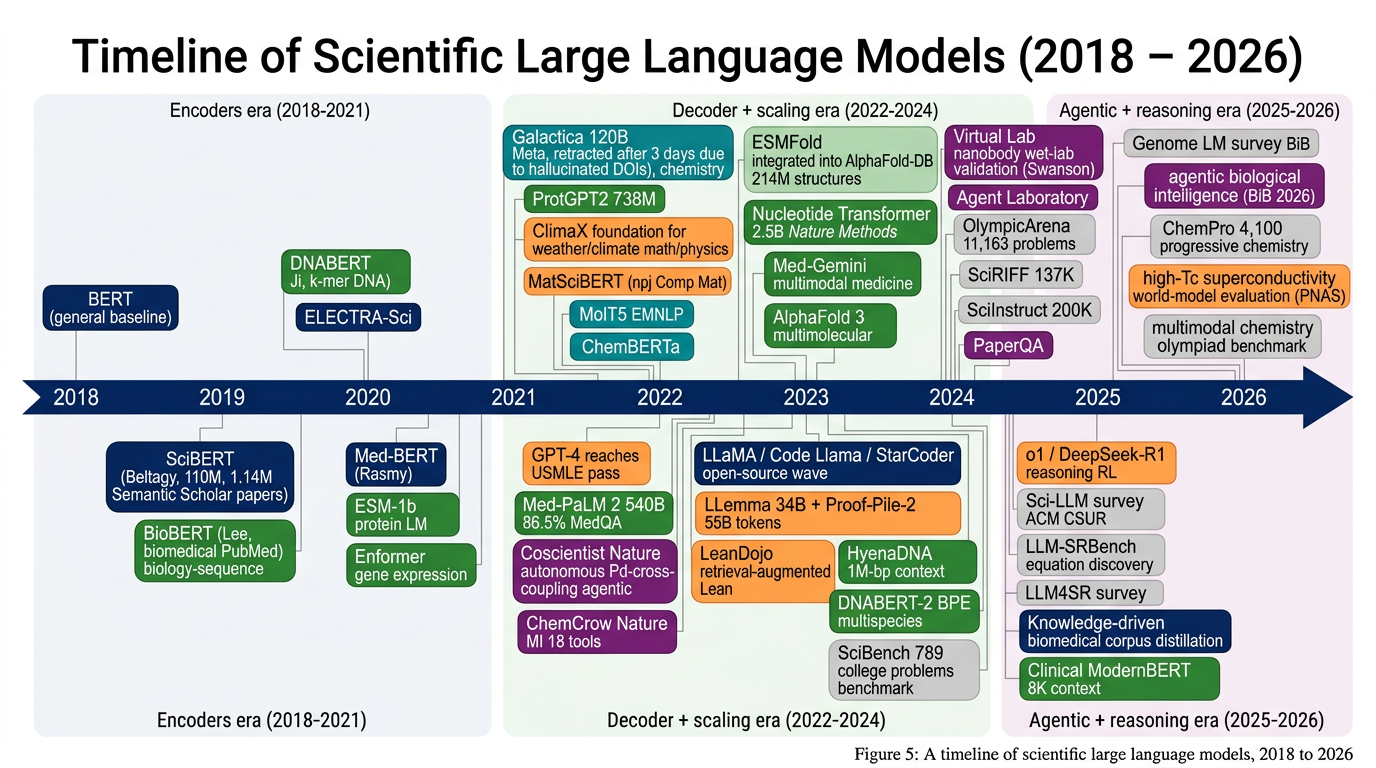
\includegraphics[keepaspectratio,alt={Timeline of Scientific Large Language Models from 2018 to 2026, organized into three swimlanes: encoder era, decoder and scaling era, and agentic and reasoning era.}]{./figures/Scientific-Large-Language-Models__fig5_timeline.png}}
\caption{Timeline of Scientific Large Language Models from 2018 to 2026, organized into three swimlanes: encoder era, decoder and scaling era, and agentic and reasoning era.}
\end{figure}

\subsection{Encoder-era foundations (2018--2021)}\label{encoder-era-foundations-20182021}

BERT's 2018 release made domain retraining an obvious move. \textbf{SciBERT} (Beltagy, Lo, Cohan, March 2019) pretrained on 1.14M Semantic Scholar papers (≈3.17B tokens) with the new 30K-WordPiece SciVocab and reported SOTA F1 on BC5CDR chemical--disease NER, ChemProt relation extraction, and SciERC, with up to +3.5 F1 over BERT-base {[}15{]}. In parallel, \textbf{BioBERT} (Lee et al., 2019) continued BERT-base pretraining on 4.5B PubMed-abstract tokens and 13.5B PMC full-text tokens, gaining +0.62 F1 on biomedical NER and beating prior baselines on BC2GM and JNLPBA {[}14{]}. Peng et al.'s \textbf{BLUE} benchmark then standardised evaluation across ten biomedical datasets {[}BLUE{]}. \textbf{Med-BERT} (Rasmy et al., \emph{npj Digital Medicine} 2021) ported the recipe to longitudinal EHRs over 28M patient records, lifting rare-disease prediction AUROC by 1.7--6.5 points {[}Med-BERT{]}. \textbf{MatSciBERT} (Gupta et al., \emph{npj Computational Materials} 2022) trained on ≈1M materials abstracts and gained +6 F1 on materials NER {[}22{]}, while early protein LMs such as \textbf{ESM-1b} (Rives et al.) showed that masked-LM on amino-acid sequences yielded embeddings that improved structure prediction. The era was \emph{encoder-only} and \emph{discriminative}: outputs were classifications, spans, or embeddings --- never free-form scientific text.

Two structural limits motivated the next phase. Encoders cannot generate, so they cannot explain, summarise, hypothesise, or plan experiments. And SciBERT's 3.17B tokens were already dwarfed by GPT-3's 300B tokens and by the trillion-token open releases that followed. By 2021 the field needed decoders, much larger corpora, and instruction-following.

\subsection{Decoder-era turning points (2022--2024)}\label{decoder-era-turning-points-20222024}

The decoder era opens with two near-simultaneous events. In November 2022 Meta AI released \textbf{Galactica}. Galactica shipped decoder-only checkpoints at 1.3B, 6.7B, 30B, and 120B parameters, trained on a curated 106B-token corpus of papers, textbooks, encyclopedias, and reference data, with explicit citation tokens and \texttt{\textless{}work\textgreater{}} working-memory tokens {[}1{]}. Galactica reached 68.2\% on MMLU science at 120B and was the first model marketed as ``a large language model for science.'' Its public demo was retracted within three days because users elicited fluent but fabricated citations and unsafe medical claims. That retraction is the canonical failure case of the era. It crystallised the field's emphasis on grounding, retrieval, and provenance --- themes later embodied in PaperQA {[}6{]} and Almanac {[}7{]}. The weights remain publicly available and were continued into \textbf{GeoGalactica} (65B geoscience tokens) {[}33{]} and \textbf{BioGPT}.

The medical decoder line opened in parallel. \textbf{Med-PaLM} (Singhal et al., \emph{Nature} 2023) reported 67.6\% on MedQA --- more than 17 points above the prior SOTA and crossing the conventional 60\% USMLE-pass threshold {[}18{]}. \textbf{Med-PaLM 2} (\emph{Nature Medicine} 2025) reached 86.5\% MedQA, 72.3\% MedMCQA, and 81.8\% PubMedQA on a 540B Flan-PaLM-2 backbone with medical instruction tuning and clinician-preference RLHF; the long-form rubric scored nine axes including factuality, harm, and bias {[}11{]}. \textbf{Med-Gemini} (Yang et al., 2024) extended the line to multimodal radiology, dermatology, ophthalmology, pathology, and genomics {[}29{]}. Community open models --- \textbf{PMC-LLaMA}, \textbf{BioMistral}, \textbf{PubMedGPT 2.7B}, and the 8K-context \textbf{Clinical ModernBERT} (Lee et al., 2025) {[}34{]} --- fill the on-prem niche.

The biological-sequence subfield matured in parallel. \textbf{ESM-2} (Lin et al., \emph{bioRxiv} 2022; later \emph{Science}) scaled protein LMs to 15B parameters on UR50/D's ≈65M sequence clusters; the paired \textbf{ESMFold} decoder predicts atomic-level structure in a single forward pass at ≈60× AlphaFold-2 speed on single chains {[}25{]}. \textbf{ProtGPT2} (Ferruz et al., 2022; 738M) generates novel proteins whose order/disorder statistics match natural proteins {[}35{]}. \textbf{DNABERT} (Ji et al., 2020; k-mers) and \textbf{DNABERT-2} (Zhou et al., 2023; multispecies BPE) cover the genome at single-base resolution; DNABERT-2 trims parameters by ≈28\% while reaching SOTA on 24/28 GUE tasks {[}23, 24{]}. \textbf{Nucleotide Transformer} (Dalla-Torre et al., \emph{Nature Methods} 2024) scales to 2.5B parameters across 850 species {[}26{]}. \textbf{HyenaDNA} (Nguyen et al., 2023) extends context to 1M base pairs at single-nucleotide resolution via a Hyena/SSM mixer {[}27{]}, and \textbf{Enformer} (Avsec et al., 2021) handles gene-expression prediction with long-range attention up to 200 kb {[}28{]}.

Chemistry expanded along an analogous arc. \textbf{MolT5} (Edwards et al., 2022) introduced bidirectional translation between natural language and SMILES, trained on ZINC-15 plus C4 {[}36{]}. \textbf{MolXPT} wrapped molecules with text for generative pretraining {[}37{]}; \textbf{MolCA} added 2D graph perception via a cross-modal projector {[}38{]}; \textbf{BioT5} unified SELFIES, FASTA, and natural language {[}39{]}; \textbf{nach0} (Livne et al., \emph{Chemical Science} 2024) is a multimodal natural+chemical foundation model {[}40{]}. 2023 was the agentic watershed: Boiko et al.'s \textbf{Coscientist} (\emph{Nature}) combined GPT-4 with planning, execution, and analysis modules to run autonomous Pd-catalysed cross-coupling on a robot {[}8{]}, while M. Bran et al.'s \textbf{ChemCrow} (\emph{Nature Machine Intelligence} 2024) wrapped GPT-4 with 18 expert tools (RDKit, IBM RXN, SMARTS, retrosynthesis) and autonomously synthesised three novel insect repellents and a 3-step novel reaction {[}12{]}.

The mathematical sciences arrived almost concurrently. \textbf{Minerva} (Lewkowycz et al., 2022; 540B PaLM fine-tuned on arXiv math) reported strong MATH and GSM8K scores. \textbf{Llemma} (Azerbayev et al., 2023) was the open analogue: 7B and 34B continued from Code Llama on \textbf{Proof-Pile-2} (55B tokens of math papers, math web, and proof code), reaching 25.0\% pass@1 on MATH at 34B {[}16{]}. \textbf{LeanDojo} (Yang et al., 2023) couples retrieval with theorem proving over 98K Lean theorems {[}17{]}, and \textbf{ProofNet} (Azerbayev et al., 2023) released 371 undergraduate Lean autoformalization problems {[}41{]}.

By 2024 the field absorbed open-source momentum from \textbf{LLaMA} (7B--65B) {[}42{]}, \textbf{Code Llama} (7B--70B) {[}43{]}, and \textbf{StarCoder} (15.5B, 1T tokens, 80+ languages) {[}44{]}, each of which became a base for scientific continuations.

\subsection{Agentic and reasoning-tuned generation (2025--2026)}\label{agentic-and-reasoning-tuned-generation-20252026}

The third inflection began in late 2024 with OpenAI's \textbf{o1} family and consolidated in 2025 with \textbf{DeepSeek-R1} (671B MoE), \textbf{QwQ}, and Google's \textbf{Gemini-Thinking}. These models apply reinforcement learning to reasoning \emph{traces} rather than final answers, lifting \textbf{GPQA-Diamond} (198 graduate-level questions) {[}GPQA{]} from low-50\% (GPT-4o) into the high-70\% range and pushing AIME scores past 80\%. The reasoning-RL paradigm is mapped in \emph{Reasoning Language Models: A Blueprint} {[}Besta{]}. In parallel, \textbf{Agent Laboratory} (Schmidgall et al., 2025) decomposed scientific research into Lit-Review, Plan, Experiment, and Report sub-agents {[}20{]}; \textbf{Virtual Lab} (Swanson et al., 2024) deployed multi-agent design of nanobodies later validated experimentally {[}19{]}; the \textbf{Sakana AI Scientist} demonstrated end-to-end short-form ML papers at ≈\$15 each; and \textbf{MASLab} {[}MASLab{]} consolidated multi-agent codebases for reproducibility.

The 2025--2026 surveys formalise this trajectory. Zhang et al.~(\emph{ACM Computing Surveys} 2025) {[}2{]} catalogues 250+ Sci-LLMs in biological and chemical domains. \emph{LLM4SR} (Luo et al., 2025) {[}4{]} groups Sci-LLMs by hypothesis generation, experiment design, content generation, and evaluation. \emph{From Automation to Autonomy} (Zheng et al., \emph{EMNLP} 2025) {[}21{]} proposes a five-level autonomy ladder. \emph{From AI for Science to Agentic Science} (Wei et al., 2025) {[}5{]} foregrounds agentic loops. Hu et al.~(2025) {[}30{]} argues that data quality, not parameter count, will be the dominant 2026--2028 bottleneck.

\subsection{Quantitative milestones}\label{quantitative-milestones}

{\def\LTcaptype{none} % do not increment counter
\begin{longtable}[]{@{}
  >{\raggedright\arraybackslash}p{(\linewidth - 6\tabcolsep) * \real{0.0426}}
  >{\raggedright\arraybackslash}p{(\linewidth - 6\tabcolsep) * \real{0.2872}}
  >{\raggedright\arraybackslash}p{(\linewidth - 6\tabcolsep) * \real{0.1809}}
  >{\raggedright\arraybackslash}p{(\linewidth - 6\tabcolsep) * \real{0.4894}}@{}}
\toprule\noalign{}
\begin{minipage}[b]{\linewidth}\raggedright
Year
\end{minipage} & \begin{minipage}[b]{\linewidth}\raggedright
Milestone
\end{minipage} & \begin{minipage}[b]{\linewidth}\raggedright
Scale
\end{minipage} & \begin{minipage}[b]{\linewidth}\raggedright
Key claim
\end{minipage} \\
\midrule\noalign{}
\endhead
\bottomrule\noalign{}
\endlastfoot
2019 & SciBERT {[}15{]} & 110M & +3.5 F1 over BERT-base on SciIE \\
2019 & BioBERT {[}14{]} & 110M & +0.62 F1 biomedical NER \\
2021 & Enformer {[}28{]} & 252M & +0.16 Pearson r on gene-expression \\
2022 & Galactica 120B {[}1{]} & 120B & 68.2\% MMLU-Sci, retracted in 3 days \\
2022 & ESM-2 15B {[}25{]} & 15B & 60× faster ESMFold vs AlphaFold 2 \\
2022 & ProtGPT2 {[}35{]} & 738M & First generative protein LM \\
2023 & Med-PaLM 2 {[}11{]} & 540B & 86.5\% MedQA \\
2023 & Coscientist {[}8{]} & GPT-4-driven & Autonomous Pd cross-coupling \\
2023 & Llemma 34B {[}16{]} & 34B & 25.0\% MATH pass@1 \\
2024 & Nucleotide Transformer {[}26{]} & 2.5B & 850-species genomic foundation \\
2024 & HyenaDNA {[}27{]} & up to 6.6M & 1M-bp single-nucleotide context \\
2024 & Virtual Lab {[}19{]} & multi-agent & Wet-lab-validated nanobodies \\
2025 & Agent Laboratory {[}20{]} & multi-agent & End-to-end research pipeline \\
2025 & o1 / DeepSeek-R1 & unreleased / 671B & Reasoning-RL crosses GPQA-Diamond expert level \\
2026 & High-Tc LLM eval {[}13{]} & GPT-4 family & Expert audit of Sci-LLM world models \\
\end{longtable}
}

The historical lesson is that each era was triggered by one architectural change plus one data change. Encoders plus domain corpora gave us SciBERT and BioBERT. Decoders plus 100B-token science corpora gave us Galactica and Med-PaLM. Reasoning RL plus agentic loops gave us Coscientist and o1-class systems. The next era, mapped in §12, will likely be triggered by closed-loop wet-lab data plus verified-grounding training objectives.

This historical scaffolding sets up the cross-cutting taxonomy of §3.

\section{Taxonomy of Sci-LLMs across Domains and Architectures}\label{taxonomy-of-sci-llms-across-domains-and-architectures}

Building on the historical trajectory of Section 2, this section fixes the taxonomy used throughout the rest of the survey along four orthogonal axes --- Domain, Architecture, Training stage, and Modality/Autonomy --- that together locate 250+ documented Sci-LLMs.

A useful Sci-LLM taxonomy cuts along multiple axes simultaneously, because the same model --- say \textbf{BioT5} --- is at once a chemistry/biology model (domain), an encoder--decoder (architecture), and a trimodal SELFIES+FASTA+text model (modality). Figure 2 organises the literature along four axes --- Domain, Architecture, Training Stage, and Modality/Autonomy --- that we use for the rest of the survey. Mutually exclusive partitions within each axis make any model locatable in a single (D, A, T, M) tuple.

\begin{figure}
\centering
\pandocbounded{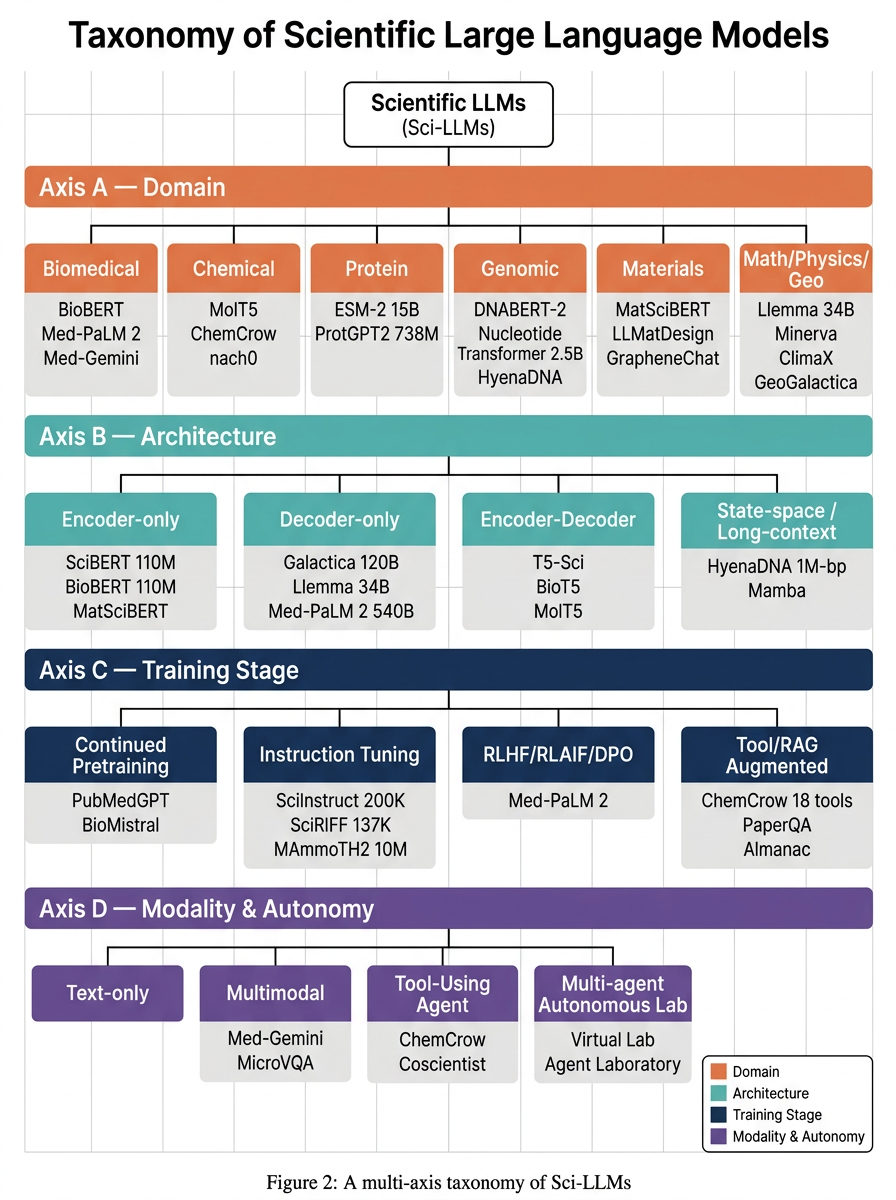
\includegraphics[keepaspectratio,alt={Taxonomy of Scientific Large Language Models along four axes: domain, architecture, training stage, and modality/autonomy.}]{./figures/Scientific-Large-Language-Models__fig2_taxonomy.png}}
\caption{Taxonomy of Scientific Large Language Models along four axes: domain, architecture, training stage, and modality/autonomy.}
\end{figure}

\subsection{Domain-axis taxonomy: biomedical, chemical, biological-sequence, mathematical, geoscientific, materials}\label{domain-axis-taxonomy-biomedical-chemical-biological-sequence-mathematical-geoscientific-materials}

The encoder lineage opened with SciBERT (2019) on 1.14M papers {[}15{]} and BioBERT (2019) on PubMed and PMC {[}14{]}, with MatSciBERT (2022) porting the recipe to materials {[}22{]}. The decoder line was launched by Galactica (2022; 120B; 106B scientific tokens) {[}1{]} and consolidated in biomedicine by Med-PaLM (2023; 540B; 67.6\% MedQA) {[}18{]}, Med-PaLM 2 (2025; clinician-RLHF; 86.5\% MedQA) {[}11{]}, and the multimodal Med-Gemini (2024) {[}29{]}. The biological-sequence side is anchored by ESM-2 (2022; 15B protein LM) {[}25{]}, DNABERT-2 (2023; BPE multispecies DNA LM) {[}24{]}, Nucleotide Transformer (2024; 850-species genomic foundation) {[}26{]}, and HyenaDNA (2023; 1M-bp single-nucleotide context) {[}27{]}. The mathematical and geoscientific branches contributed Llemma (2023; 34B math LM continued from Code Llama) {[}16{]}, LeanDojo (2023; retrieval-augmented Lean prover) {[}17{]}, ClimaX (2023; ViT on CMIP6) {[}52{]}, and GeoGalactica (2023; 65B-token geoscience continuation) {[}33{]}. The biomedical branch is the largest by paper count: BioBERT (110M) {[}14{]}, SciBERT (110M) {[}15{]}, PMC-LLaMA, BioMistral 7B, PubMedGPT 2.7B, Clinical ModernBERT (Lee et al., 2025; 8K context) {[}34{]}, the \textbf{Med-PaLM} family --- Med-PaLM (540B Flan-PaLM base, 67.6\% MedQA {[}18{]}) and Med-PaLM 2 (86.5\% MedQA {[}11{]}) --- and the multimodal \textbf{Med-Gemini} {[}29{]}. Sahoo et al.'s 2024 JAMIA review {[}Sahoo{]} and Tian et al.'s \emph{Briefings in Bioinformatics} survey {[}45{]} inventory more than 80 biomedical Sci-LLMs and catalogue their failure modes on clinical-note tasks.

The \textbf{chemical} branch contains MolT5 {[}36{]}, MolXPT {[}37{]}, MolCA {[}38{]}, BioT5 {[}39{]}, nach0 {[}40{]}, the agentic \textbf{ChemCrow} with its 18-tool catalogue {[}12{]}, and \textbf{ChemToolAgent} for tool-impact analysis {[}46{]}. Ramos et al.'s 2024 \emph{Chemical Science} review {[}47{]} groups these into five chemistry tasks: molecule design, property prediction, retrosynthesis, reaction-condition prediction, and synthesis planning. The \textbf{ChemPro} benchmark (Baranwal \& Vyas, 2026) {[}48{]} tests 4,100 progressive chemistry questions across four difficulty tiers, providing a non-saturated successor to ChemBench {[}Guo2023chembench{]}.

The \textbf{biological-sequence} branch contains protein LMs (ESM-1b, ESM-2 at 15B {[}25{]}, ProtGPT2 at 738M {[}35{]}), DNA LMs (DNABERT {[}23{]}, DNABERT-2 {[}24{]}, Nucleotide Transformer 2.5B {[}26{]}, HyenaDNA up to 1.6B parameters and 1M-bp context {[}27{]}), gene-expression models (Enformer {[}28{]}), and RNA LMs including Zhang et al.'s MSA-based model in \emph{Nucleic Acids Research} 2023 {[}49{]}. Shu et al.'s 2026 genome-LM survey {[}50{]} covers 60+ models, and Yang et al.'s 2026 ESM-applications survey {[}Yang2026ESM{]} documents binder design, function prediction, structure prediction, and stability prediction as the dominant downstream uses. Crucially, biological-sequence Sci-LLMs \emph{do not consume natural language} during pretraining; that asymmetry motivates the four-axis taxonomy and the bridging models (BioT5, Med-Gemini) of §3.4.

The \textbf{mathematical and physics} branch contains \textbf{Minerva} (540B PaLM math-tuned, 50.3\% MATH), \textbf{Llemma} (7B/34B continued from Code Llama on 55B-token Proof-Pile-2; 25.0\% MATH pass@1) {[}16{]}, \textbf{LeanDojo} (retrieval-augmented Lean over 98K theorems) {[}17{]}, \textbf{ProofNet} (371 undergraduate autoformalization problems) {[}41{]}, and reasoning-RL successors o1, DeepSeek-R1, QwQ, and Gemini-Thinking. Ahn et al.'s 2024 EACL survey {[}Ahn{]} groups them into formal-proof, problem-solving, and equation-discovery sub-branches; \textbf{LLM-SRBench} {[}51{]} formalises the equation-discovery axis.

The \textbf{geoscientific} branch contains \textbf{ClimaX} (Nguyen et al., 2023; Vision Transformer pretrained on CMIP6 reanalysis) {[}52{]} and \textbf{GeoGalactica} (Lin et al., 2023; 65B-token continuation of Galactica) {[}33{]}. Zhao et al.'s 2024 \emph{The Innovation} review {[}53{]} identifies remote-sensing, hydrology, and climate as the three main verticals.

The \textbf{materials} branch contains \textbf{MatSciBERT} (\emph{npj Comp Mat} 2022) {[}22{]}, \textbf{LLMatDesign} (Jia et al., 2024) {[}54{]}, \textbf{GrapheneChat} {[}GrapheneChat{]}, and the high-Tc-superconductivity world-model evaluation of Guo et al.~(\emph{PNAS} 2026) {[}13{]}. Wang et al.'s 2025 review in \emph{Review of Materials Research} {[}55{]} argues that the binding constraint for materials Sci-LLMs is structured-data extraction from PDFs, not model scale.

The \textbf{general-science} branch --- Galactica {[}1{]}, SciInstruct {[}9{]}, SciRIFF {[}10{]}, MAmmoTH2 {[}56{]} --- covers models that span all domains and serves as the source of broad instruction-tuning corpora.

\subsection{Architecture-axis taxonomy: encoder, decoder, encoder--decoder, state-space}\label{architecture-axis-taxonomy-encoder-decoder-encoderdecoder-state-space}

\textbf{Encoder-only} Sci-LLMs (SciBERT, BioBERT, MatSciBERT, Clinical ModernBERT) optimise masked LM and excel at NER, classification, and embeddings; they sit at 110M--340M parameters and run on a single A100. \textbf{Decoder-only} Sci-LLMs (Galactica 120B, Med-PaLM 2 540B, Llemma 34B, Med-Gemini) optimise causal LM and produce free-form generations; they dominate the 2023--2026 headlines. \textbf{Encoder--decoder} Sci-LLMs (BioT5, MolT5, T5-Sci) optimise span corruption and dominate translation tasks (text↔SMILES, FASTA↔text, summarization). \textbf{State-space and long-context} architectures --- HyenaDNA up to 1M-bp context {[}27{]}, Mamba 2.8B {[}Mamba{]}, Striped-Mamba bio variants --- trade quadratic attention for linear-time selective state-space mixers, delivering ≈5× higher throughput at long contexts and unlocking whole-genome modeling.

\subsection{Training-stage taxonomy: continued PT, instruction tuning, RLHF, tool/RAG augmentation}\label{training-stage-taxonomy-continued-pt-instruction-tuning-rlhf-toolrag-augmentation}

Four post-pretraining stages organise the field. \textbf{Continued pretraining} adapts a general LLM (LLaMA-2, Code Llama) to a domain corpus while preserving general competence --- the recipe behind PMC-LLaMA, BioMistral, GeoGalactica, and Llemma. \textbf{Instruction tuning} aligns the model with task formats: SciInstruct (200K self-reflective instructions across math, chemistry, physics, biology) {[}9{]}, SciRIFF (137K instructions across 54 tasks, including dataset extraction, claim verification, and IE) {[}10{]}, MAmmoTH2 (10M reasoning instructions mined from web) {[}56{]}. \textbf{Preference alignment} via RLHF, RLAIF, or DPO follows: Med-PaLM 2 used clinician preferences over candidate answers {[}11{]}; the chemistry literature {[}47{]} increasingly uses RLAIF with a stronger LLM as judge. \textbf{Tool and retrieval augmentation} pulls knowledge at inference time: PaperQA {[}6{]} couples dense retrieval, citation-graph traversal, and evidence summarisation; Almanac (\emph{NEJM AI} 2024) {[}7{]} retrieves clinical guidelines and lifts factuality to 91\% versus ChatGPT's 64\% on the same set; ChemCrow {[}12{]} dispatches among 18 chemistry tools.

\subsection{Modality and autonomy axis}\label{modality-and-autonomy-axis}

By \textbf{modality}, Sci-LLMs span text-only (SciBERT, Llemma), text+SMILES (MolT5), graph+text (MolCA), DNA+protein+text (BioT5), and image+text+structured (Med-Gemini, MicroVQA-tuned models). By \textbf{autonomy}, the spectrum runs from passive QA models (Med-PaLM, Galactica), to tool-using single agents (ChemCrow, Coscientist), to multi-agent autonomous laboratories (Virtual Lab {[}19{]}, Agent Laboratory {[}20{]}), to goal-evolving agents that update their own scientific objectives {[}66{]}. Wei et al.'s 2025 five-level autonomy ladder L0--L5 {[}5{]} formalises this axis.

\subsection{Cross-axis comparison table}\label{cross-axis-comparison-table}

The matrix below cross-references representative Sci-LLMs along Domain × Architecture × Training stage × Modality/Autonomy. Readers asking which model fits a particular cell should consult Table 3.1 first; subsections §3.6 and §8 then drill in.

{\def\LTcaptype{none} % do not increment counter
\begin{longtable}[]{@{}
  >{\raggedright\arraybackslash}p{(\linewidth - 10\tabcolsep) * \real{0.2319}}
  >{\raggedright\arraybackslash}p{(\linewidth - 10\tabcolsep) * \real{0.1087}}
  >{\raggedright\arraybackslash}p{(\linewidth - 10\tabcolsep) * \real{0.1377}}
  >{\raggedright\arraybackslash}p{(\linewidth - 10\tabcolsep) * \real{0.2826}}
  >{\raggedright\arraybackslash}p{(\linewidth - 10\tabcolsep) * \real{0.1667}}
  >{\raggedright\arraybackslash}p{(\linewidth - 10\tabcolsep) * \real{0.0725}}@{}}
\toprule\noalign{}
\begin{minipage}[b]{\linewidth}\raggedright
Model
\end{minipage} & \begin{minipage}[b]{\linewidth}\raggedright
Domain
\end{minipage} & \begin{minipage}[b]{\linewidth}\raggedright
Architecture
\end{minipage} & \begin{minipage}[b]{\linewidth}\raggedright
Training stage
\end{minipage} & \begin{minipage}[b]{\linewidth}\raggedright
Modality/Autonomy
\end{minipage} & \begin{minipage}[b]{\linewidth}\raggedright
Params
\end{minipage} \\
\midrule\noalign{}
\endhead
\bottomrule\noalign{}
\endlastfoot
SciBERT {[}15{]} & General-science & Encoder & Pretrain on 1.14M papers & Text & 110M \\
BioBERT {[}14{]} & Biomedical & Encoder & Continued PT on PubMed & Text & 110M \\
MatSciBERT {[}22{]} & Materials & Encoder & Continued PT on 1M materials abstracts & Text & 110M \\
Galactica 120B {[}1{]} & General-science & Decoder & Pretrain on 106B-token sci corpus & Text + LaTeX + SMILES & 120B \\
Med-PaLM 2 {[}11{]} & Biomedical & Decoder & Instruction + RLHF on Flan-PaLM 2 & Text & 540B \\
Llemma 34B {[}16{]} & Math & Decoder & Continued PT on Proof-Pile-2 & Text + LaTeX + code & 34B \\
ESM-2 15B {[}25{]} & Protein & Encoder & Pretrain on UR50 65M & Amino acids & 15B \\
ProtGPT2 {[}35{]} & Protein & Decoder & Pretrain on UniRef50 & Amino acids & 738M \\
DNABERT-2 {[}24{]} & Genomic & Encoder & Pretrain multispecies + BPE & DNA & 117M \\
Nucleotide Transformer 2.5B {[}26{]} & Genomic & Encoder & Pretrain 850 species & DNA & 2.5B \\
HyenaDNA {[}27{]} & Genomic & SSM & Pretrain on human genome & DNA, 1M-bp ctx & 6.6M--1.6B \\
MolT5 {[}36{]} & Chemistry & Encoder--decoder & Pretrain ZINC + C4 & Text + SMILES & 250M--800M \\
BioT5 {[}39{]} & Bio + Chem & Encoder--decoder & Pretrain trimodal & Text + SELFIES + FASTA & 252M \\
nach0 {[}40{]} & Chemistry & Encoder--decoder & Multitask & Text + SMILES & 770M \\
ChemCrow {[}12{]} & Chemistry & Decoder + tools & GPT-4 + 18 tools & Tool-using agent & -- \\
Coscientist {[}8{]} & Chemistry & Decoder + tools & GPT-4 + 4 modules & Multi-component agent & -- \\
Virtual Lab {[}19{]} & Biology & Multi-agent & GPT-4 PI + scientists + critic & Multi-agent & -- \\
Agent Laboratory {[}20{]} & General & Multi-agent & Lit-Review + Plan + Experiment + Report & Multi-agent & -- \\
ClimaX {[}52{]} & Climate & ViT & Pretrain on CMIP6 & Spatial weather & 200M \\
GeoGalactica {[}33{]} & Geoscience & Decoder & Continued PT 65B geoscience tokens & Text & 30B \\
Med-Gemini {[}29{]} & Biomedical & Multimodal decoder & Instruction tuning Gemini & Text + image + genomics & unreleased \\
Clinical ModernBERT {[}34{]} & Biomedical & Encoder & 8K context biomedical & Text & 150M \\
LLMatDesign {[}54{]} & Materials & Decoder + tools & LLM-driven & Tool-using & -- \\
Llemma + LeanDojo {[}16,17{]} & Math & Decoder + retrieval & Lean tactic retrieval & Text + Lean & 34B \\
\end{longtable}
}

\subsection{What this taxonomy makes obvious}\label{what-this-taxonomy-makes-obvious}

Three patterns become legible only after cross-tabulation. First, \textbf{agentic Sci-LLMs are still rare}: the majority of models live in the (Decoder, Continued-PT, Text) cell, and the (Multi-agent, Closed-loop) cells are populated by fewer than 30 documented systems. Second, the \textbf{bio-sequence diagonal} --- protein and DNA LMs --- is structurally different because natural-language input is absent during pretraining; the natural-language reasoning available to Galactica or Med-PaLM is therefore unavailable, and bridging models such as BioT5 and Med-Gemini exist specifically to plug that gap. Third, the \textbf{autonomy frontier} is dominated by GPT-4-class proprietary backbones (Coscientist, ChemCrow, Virtual Lab, Agent Laboratory), so the field is vulnerable to closed-API risk; open-weights agentic systems remain a 2026 frontier.

This taxonomy underwrites the rest of the survey: §4 covers algorithmic mechanism (Architecture × Training stage); §5 covers alignment and reasoning; §§6--7 cover tool/retrieval augmentation and multi-agent autonomy; §8 walks each domain branch in depth.

\section{Algorithmic Mechanisms for Domain-Adapted Pretraining}\label{algorithmic-mechanisms-for-domain-adapted-pretraining}

Building on the taxonomy in Section 3, this section turns to the algorithmic mechanisms behind domain-adapted Sci-LLM pretraining: tokenization, pretraining objectives, scaling, continued-PT recipes, long-context architectures, tool-augmented inference, and inference-cost trade-offs.

A Sci-LLM shares its algorithmic core with general LLMs --- a transformer optimising a likelihood objective on tokens --- but the \emph{details that matter} for science differ: tokenization, corpus mix, objectives that admit citations and step-by-step working memory, long-context architectures for genomes, and continued-pretraining recipes that avoid catastrophic forgetting. This section examines those mechanisms in depth, with concrete numbers wherever the literature reports them.

\subsection{Domain tokenization: SciVocab, SMILES BPE, k-mer/BPE genomes}\label{domain-tokenization-scivocab-smiles-bpe-k-merbpe-genomes}

Tokenization is the first lever that distinguishes Sci-LLMs from general LLMs. The encoder-era benchmark is SciVocab (2019; 30K WordPiece on 1.14M papers; +3.5 SciIE F1) {[}15{]}. Galactica (2022) adopted a custom mixed BPE with citation and \texttt{\textless{}work\textgreater{}} tokens {[}1{]}. DNABERT (2020) used overlapping k-mers at k = 3--6 {[}23{]} before DNABERT-2 (2023) replaced them with multispecies BPE, cutting parameters by 28\% and adding +5 F1 on GUE {[}24{]}. HyenaDNA (2023) abandoned tokenization altogether by operating on single nucleotides at 1M-bp context {[}27{]}, while ESM-2 (2022) uses a 25-token amino-acid alphabet {[}25{]}. On the chemistry side, MolT5 (2022) applied SentencePiece to SMILES {[}36{]} and BioT5 (2023) switched to SELFIES for validity-by-construction {[}39{]}. MatSciBERT (2022; WordPiece on materials abstracts; +6 NER F1) {[}22{]} and Mswahili \& Jeong's 2024 SELFIES+RoBERTa pipeline (top SMILES validity rates) {[}Mswahili{]} close the inventory. The first lever is tokenization. SciBERT introduced \textbf{SciVocab} --- a 30K-token WordPiece vocabulary learned over its 1.14M-paper corpus --- and reported that 42\% of biomedical entities became single tokens versus only 15\% under BERT's WikiVocab; the paper attributes its +3.5 F1 SciIE gain over BERT-base primarily to this tokenizer change {[}15{]}. Galactica adopted a custom mixed BPE that segments LaTeX macros, SMILES atoms, and DOIs as atomic units; the \texttt{\textless{}work\textgreater{}} token and \texttt{{[}\$START\_R\$EF{]}}/\texttt{{[}\$END\_R\$EF{]}} citation tokens are ordinary BPE tokens whose embeddings are co-trained with the rest {[}1{]}. DNABERT used overlapping k-mers (k = 3, 4, 5, 6); DNABERT-2 {[}24{]} showed that k-mers create vocabulary redundancy and replaced them with byte-pair encoding, cutting parameters by ≈28\% while improving 24 of 28 GUE tasks. HyenaDNA {[}27{]} sidesteps tokenization altogether by operating at single-nucleotide resolution and relying on the Hyena/SSM mixer to model dependencies up to 1M base pairs. ESM-2 {[}25{]} uses 25 single-character amino-acid tokens (20 residues plus B, J, O, U, X, Z, mask), and its structural performance scales smoothly from 8M to 15B parameters.

For chemistry, tokenization choice lies among SMILES, SELFIES (parse-validity by construction), and InChI. MolT5 {[}36{]} uses SentencePiece over SMILES; BioT5 {[}39{]} switched to SELFIES because invalid SMILES were a top failure mode. Mswahili \& Jeong (\emph{Heliyon} 2024) {[}Mswahili{]} document that SELFIES + RoBERTa-style pretraining yields the most stable validity rates in molecule-caption translation. Tokenization is therefore a first-class design parameter, not a hyperparameter.

\subsection{Pretraining objectives, scaling, and continued-PT recipes}\label{pretraining-objectives-scaling-and-continued-pt-recipes}

Pretraining objectives split cleanly by architecture. Encoder-only Sci-LLMs use masked-language modelling (MLM) with the standard 15\% mask rate. Decoder-only Sci-LLMs use causal next-token prediction. Encoder--decoder Sci-LLMs (BioT5, MolT5) use span corruption. Galactica adds \texttt{\textless{}work\textgreater{}} tokens to its causal LM objective so that multi-step reasoning becomes explicit during training, and upweights working-memory and citation tokens in the loss; ablations in Taylor et al.~{[}1{]} show that removing citation tokens drops citation prediction by ≈15 BLEU points.

Scaling laws follow Chinchilla optimality with one important deviation: \textbf{domain-corpus scaling plateaus earlier}. Llemma {[}16{]} reports that continuing Code Llama 34B on 55B Proof-Pile-2 tokens lifts MATH pass@1 from 14.0\% to 25.0\%, but doubling to 110B tokens yields only a further 1.3-point gain --- diminishing returns set in at roughly 5--10× the original corpus size. For Med-PaLM 2 {[}11{]}, clinician-RLHF mostly improves long-form rubric scores (factuality, harm) rather than MedQA accuracy, suggesting that preference data, not tokens, is now binding.

Continued-PT recipes converge on a near-universal schedule: warm-start from a strong general checkpoint, lower the learning rate by ≈10× (typically 3e-4 → 1e-5), preserve 5--10\% general data to mitigate catastrophic forgetting, and run 1--3 epochs over the domain corpus. Llemma {[}16{]}, BioMistral, PMC-LLaMA, and GeoGalactica {[}33{]} all follow this template within ±2× variance on hyperparameters.

\subsection{Long-context architectures for genomes and papers}\label{long-context-architectures-for-genomes-and-papers}

Standard transformer attention is \(O(N^2 d)\) in sequence length, which is fatal for genomes spanning 10\textsuperscript{4--10}6 bases. \textbf{HyenaDNA} {[}27{]} replaces self-attention with a Hyena mixer of long convolutions and gating, reaching \(O(N \log N)\) time and training stably over 1M-bp contexts at single-nucleotide resolution. \textbf{Mamba} {[}Mamba{]} generalises selective state-space models and achieves ≈5× higher throughput than equivalent transformers at 1M-token context. \textbf{FlashAttention-2} keeps quadratic attention but halves memory and roughly doubles throughput for normal-context Sci-LLMs (Galactica, Med-PaLM).

For long \emph{scientific papers} (often 50K+ tokens with figures and references), \textbf{Clinical ModernBERT} {[}34{]} reaches 8K context using position-interpolation and rotary embeddings, \textbf{Longformer-Sci} uses sliding-window attention, and PaperQA {[}6{]} sidesteps the problem entirely by chunking-and-retrieving rather than stretching context.

\subsection{Mechanism of tool-augmented and reasoning-augmented inference}\label{mechanism-of-tool-augmented-and-reasoning-augmented-inference}

The ReAct-style loop underlies tool-augmented Sci-LLMs. The pattern was crystallised by ReAct (2022; Thought--Action--Observation prompting) and instantiated in chemistry by ChemCrow (2024; GPT-4 + 18 chemistry tools) {[}12{]} and Coscientist (2023; GPT-4 + 4 modules + OPENTRONS robot) {[}8{]}. LLMatDesign (2024; LLM + DFT + property predictors) {[}54{]} extends the idea to materials, while LeanDojo (2023; retrieval-augmented Lean tactic prover) {[}17{]} brings it to mathematics. On the retrieval side, PaperQA (2023; dense retrieval + citation-graph traversal) {[}6{]} and Almanac (2024; curated clinical-corpus RAG) {[}7{]} anchor scientific QA. ChemToolAgent (2024; tool-impact benchmarking) {[}46{]}, BRAD (knowledge-graph-grounded biomarker agent) {[}BRAD{]}, and Agent Laboratory (2025; Lit-Review + Plan + Experiment + Report sub-agents) {[}20{]} complete the inventory. The mechanism diagram in Figure 3 captures the core of the agentic Sci-LLM loop. The reasoning module is a Sci-LLM (typically GPT-4 in Coscientist and ChemCrow {[}8, 12{]}) that emits a thought, an action over a tool catalogue, and an observation; the loop is the \textbf{ReAct} template applied to scientific tools. The tool catalogue varies by system: Coscientist exposes web search, an OPENTRONS robot, a literature summariser, and a reaction-prediction backend; ChemCrow exposes 18 chemistry tools --- RDKit, IBM RXN, Reaxys-style retrosynthesis, and SMARTS-based safety filters {[}12{]}; ChemToolAgent {[}46{]} benchmarks how tool \emph{composition} affects downstream performance and shows that ill-conditioned tools can hurt accuracy. The Sakana AI Scientist, Agent Laboratory {[}20{]}, and Virtual Lab {[}19{]} generalise the loop to scientific \emph{roles} --- PI, scientist, reviewer --- implemented as separate prompted instances of the same underlying Sci-LLM.

\begin{figure}
\centering
\pandocbounded{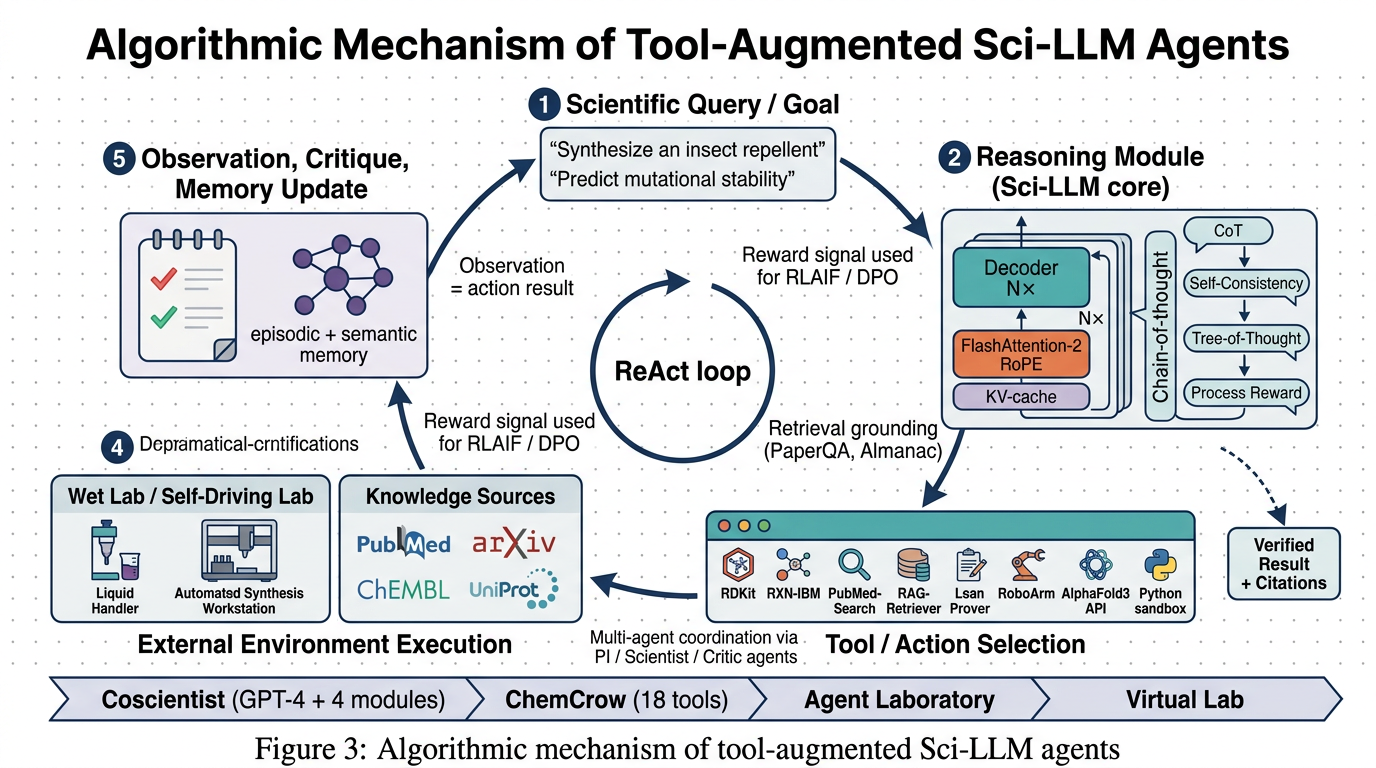
\includegraphics[keepaspectratio,alt={Algorithmic mechanism of tool-augmented Sci-LLM agents: a loop of query → reasoning → tool selection → external execution → observation and memory update.}]{./figures/Scientific-Large-Language-Models__fig3_mechanism.png}}
\caption{Algorithmic mechanism of tool-augmented Sci-LLM agents: a loop of query → reasoning → tool selection → external execution → observation and memory update.}
\end{figure}

The reasoning-enhancement stack --- chain-of-thought, self-consistency, tree-of-thought, process-reward modelling --- was originally designed for general LLMs but transfers especially well to Sci-LLMs. SciInstruct {[}9{]} explicitly trains models to produce \emph{self-reflective} reasoning chains; the authors report that ablating self-reflection drops physics-test accuracy by 6.4 points on held-out evaluation. MAmmoTH2 {[}56{]} mines 10M reasoning instructions from web corpora and gains +4.5 average points across MMLU-STEM and BBH. The reasoning-RL paradigm of o1 and DeepSeek-R1 trains the model to emit long chain-of-thought traces and rewards final correctness; Liu et al.'s 2025 RL+LLM survey {[}LiuRL{]} details the optimisation pipeline.

\subsection{Inference complexity and hardware footprint}\label{inference-complexity-and-hardware-footprint}

Galactica 120B inference at FP16 needs ≈240 GB of GPU memory, fitting on a single 8×A100-80GB node with tensor parallelism. ESM-2 15B needs ≈30 GB at FP16. Llemma 34B fits in a single 80GB A100 with int8 quantisation. The 2024 PEFT survey {[}PEFT{]} reports that LoRA at rank 8 cuts fine-tuning memory by ≈3× while losing fewer than 0.5 points on standard scientific evaluations. For closed-loop labs the binding cost is no longer GPU but \textbf{wet-lab time}: Coscientist's Pd cross-coupling {[}8{]} consumes ≈36 hours of robot time per autonomous synthesis, against ≈8 hours of LLM inference.

\subsection{Concrete algorithmic recipe in pseudocode}\label{concrete-algorithmic-recipe-in-pseudocode}

A typical Sci-LLM agentic loop, distilled from Coscientist {[}8{]}, ChemCrow {[}12{]}, and Agent Laboratory {[}20{]}, is:

\begin{verbatim}
state ← $initial_q$uery
memory ← []
for step = 1 .. K:
    thought, action, args ← LLM.generate(state, memory, tool_catalog)
    if action == FINISH: return thought
    observation ← Tool[action].run(args)
    memory.append((thought, action, args, observation))
    state ← update_state(state, observation)
\end{verbatim}

In Coscientist this loop ran with K up to 24 in autonomous chemistry tasks {[}8{]}; in Virtual Lab the loop is instantiated per agent and a moderator agent decides when to stop {[}19{]}.

\subsection{Algorithmic comparison table}\label{algorithmic-comparison-table}

{\def\LTcaptype{none} % do not increment counter
\begin{longtable}[]{@{}
  >{\raggedright\arraybackslash}p{(\linewidth - 8\tabcolsep) * \real{0.3190}}
  >{\raggedright\arraybackslash}p{(\linewidth - 8\tabcolsep) * \real{0.1810}}
  >{\raggedright\arraybackslash}p{(\linewidth - 8\tabcolsep) * \real{0.2414}}
  >{\raggedright\arraybackslash}p{(\linewidth - 8\tabcolsep) * \real{0.1121}}
  >{\raggedright\arraybackslash}p{(\linewidth - 8\tabcolsep) * \real{0.1466}}@{}}
\toprule\noalign{}
\begin{minipage}[b]{\linewidth}\raggedright
Mechanism
\end{minipage} & \begin{minipage}[b]{\linewidth}\raggedright
Representative system
\end{minipage} & \begin{minipage}[b]{\linewidth}\raggedright
Objective
\end{minipage} & \begin{minipage}[b]{\linewidth}\raggedright
Complexity
\end{minipage} & \begin{minipage}[b]{\linewidth}\raggedright
Notable result
\end{minipage} \\
\midrule\noalign{}
\endhead
\bottomrule\noalign{}
\endlastfoot
Domain MLM with SciVocab & SciBERT {[}15{]} & Masked LM & \(O(N^2 d)\) & +3.5 F1 SciIE \\
Domain causal LM with citation tokens & Galactica {[}1{]} & CausalLM + \texttt{\textless{}work\textgreater{}}, \texttt{{[}REF{]}} & \(O(N^2 d)\) & 68.2\% MMLU-Sci \\
Continued-PT on math papers & Llemma 34B {[}16{]} & CausalLM & \(O(N^2 d)\) & 25.0\% MATH \\
Span corruption + multimodal & BioT5 {[}39{]} & T5 span & \(O(N^2 d)\) & SOTA on Mol2Cap \\
Protein MLM at 15B scale & ESM-2 {[}25{]} & MLM & \(O(N^2 d)\) & ESMFold 60× speed \\
BPE multispecies DNA MLM & DNABERT-2 {[}24{]} & MLM & \(O(N^2 d)\) & +5 F1 GUE \\
Hyena SSM at 1M-bp & HyenaDNA {[}27{]} & CausalLM & \(O(N \log N)\) & 1M-bp ctx \\
Selective SSM & Mamba {[}Mamba{]} & CausalLM & \(O(N)\) & 5× throughput \\
ReAct + 18 tools & ChemCrow {[}12{]} & Tool-augmented prompting & -- & Autonomous synth \\
RAG over papers & PaperQA {[}6{]} & Dense retrieval + summarize & -- & 73\% factuality \\
RL on reasoning traces & o1, DeepSeek-R1 & RL on CoT & -- & +20 GPQA-Diamond \\
Multi-agent & Virtual Lab {[}19{]} & Role-prompted GPT-4 & -- & Wet-lab nanobody \\
\end{longtable}
}

\subsection{Why these mechanisms matter for evaluation}\label{why-these-mechanisms-matter-for-evaluation}

Algorithmic choices directly determine the metrics surveyed in §9. SciVocab and SMILES BPE determine validity rates; long-context architectures determine genome-task accuracy; citation tokens determine factuality; tool augmentation determines pass-rate on autonomous tasks. ChemToolAgent {[}46{]} sharpens the point: simply adding tools without curation can \emph{hurt} a Sci-LLM's chemistry score, because agentic systems must learn \emph{when} to call tools, not only \emph{how}. Mechanism design and benchmark design therefore co-evolve --- a theme picked up in §9 and §12.

The next section turns from pretraining mechanism to alignment, where Galactica's retraction is the canonical motivating failure.

\section{Instruction Tuning, Alignment, and Reasoning for Science}\label{instruction-tuning-alignment-and-reasoning-for-science}

Whereas Section 4 focused on pretraining mechanism, this section turns to alignment --- where Galactica's three-day retraction is the canonical motivating failure --- covering scientific instruction-tuning corpora, RLHF/RLAIF/DPO preference alignment, chain-of-thought and tree-of-thought prompting, reasoning-RL post-training, tool augmentation as alignment, safety alignment, and calibration.

A pretrained Sci-LLM is rarely deployable as is. Galactica's 2022 retraction {[}1{]} showed that fluency without alignment produces hallucinated citations and unsafe medical advice. Med-PaLM's 67.6\% MedQA was lifted to Med-PaLM 2's 86.5\% primarily through medical instruction tuning and clinician-preference RLHF, \emph{not} through additional pretraining {[}11, 18{]}. This section surveys the algorithms that turn a raw scientific decoder into an evaluator-aligned, reasoning-capable, safety-screened scientific assistant.

\subsection{Scientific instruction-tuning corpora}\label{scientific-instruction-tuning-corpora}

Instruction-tuning corpora turn raw Sci-LLM decoders into evaluator-aligned scientific assistants. The leading general-science corpora are SciInstruct (2024; 200K self-reflective instructions) {[}9{]}, SciRIFF (2024; 137K instructions across 54 tasks) {[}10{]}, and MAmmoTH2 (2024; 10M web-mined reasoning instructions) {[}56{]}. Knowledge-Driven Agentic Distillation (2025; KG-coupled biomedical IT) {[}57{]} and Proof-Pile-2 (2023; 55B math+sci tokens for Llemma) {[}16{]} target domain-specific use cases. Smaller corpora include ChemBench-IT (2023; chemistry instructions) {[}Guo2023chembench{]} and the MedInstruct medical corpus used by PMC-LLaMA, with Galactica's own pretraining mixture (2022; with \texttt{\textless{}work\textgreater{}} and \texttt{{[}REF{]}} tokens) {[}1{]} functioning as a hybrid pretraining-as-instruction corpus. \textbf{SciInstruct} (Zhang et al., 2024) released ≈200K self-reflective instruction--response pairs spanning mathematics, chemistry, physics, and biology, with each response annotated for chain-of-thought correctness. The authors report 7.4-point gains on physics MCQs and 5.1-point gains on biology MCQs over the same backbone tuned without self-reflection {[}9{]}. \textbf{SciRIFF} (Wadden et al., 2024) covers 137K instructions across 54 distinct scientific NLP tasks. The 54 tasks include dataset extraction, claim verification, and information extraction (IE) over biomedical and CS papers. SciRIFF-tuned models gain ≈28\% on average across SciRIFF-Eval. Gains concentrate on extraction tasks where instruction tuning bridges the gap between pretraining and structured output {[}10{]}. \textbf{MAmmoTH2} (Yue et al., 2024) mines 10M reasoning instructions from web corpora using a teacher LLM. It reports +4.5 average points across MMLU-STEM and BBH on a 7B base {[}56{]}. The 2025 \textbf{Knowledge-Driven Agentic Distillation} framework {[}57{]} couples a teacher LLM with a knowledge graph to distil biomedical instructions at scale, targeting the dearth of high-quality instructions in low-resource subfields. Smaller domain-specific corpora include Llemma's math-specific Proof-Pile-2 (55B tokens; continued PT rather than IT) {[}16{]} and the chemistry corpora used by ChemBench-IT {[}Guo2023chembench{]}.

\subsection{Preference alignment via RLHF, RLAIF, and DPO}\label{preference-alignment-via-rlhf-rlaif-and-dpo}

PPO-RLHF (2022; used by Med-PaLM 2 with clinician preferences) {[}11{]} is the original preference-alignment recipe, with RLAIF (2024; GPT-4 judge) {[}47{]} as the dominant chemistry alternative when domain experts are scarce. DPO (2023; closed-form contrastive over preferences; +2 over PPO on math) {[}9{]} replaces PPO with a contrastive loss. Process-Reward Modeling (2024; reward on intermediate steps; central to o1) {[}LiuRL{]} and GRPO (2025; group-relative reasoning RL used by DeepSeek-R1) define the reasoning-RL frontier. Self-Alignment for Factuality (2024; self-critique without human data) {[}SelfAlign{]}, Constitutional AI (2022; RLAIF with explicit principles), and ReST-style iterative SFT bootstrapping close the inventory. The original RLHF pipeline runs PPO over a learned reward model trained on pairwise human judgments. It was inherited from InstructGPT and applied to Med-PaLM 2 with clinician preferences {[}11{]}. Singhal et al.~2025 {[}11{]} report that on a panel of 1,066 clinicians scoring long-form answers across 9 axes (factuality, reasoning, harm, bias, helpfulness, etc.), Med-PaLM 2 was preferred over Med-PaLM on 9 of 9 axes and over physician answers on 8 of 9 axes. The chemistry literature increasingly uses \textbf{RLAIF}, a stronger LLM as judge, because clinician-grade chemistry preferences are scarce. Ramos et al.'s 2024 review {[}47{]} documents several teams using GPT-4 as critic over reaction-condition predictions. \textbf{DPO} replaces RL with a closed-form contrastive loss. SciInstruct uses DPO over self-reflective traces and gains ≈2 points over PPO on math benchmarks {[}9{]}. \textbf{Process-reward modelling} rewards correct intermediate steps rather than only final answers and is central to the o1 / DeepSeek-R1 reasoning-RL pipeline.

\subsection{Chain-of-thought, self-consistency, and tree-of-thought for science}\label{chain-of-thought-self-consistency-and-tree-of-thought-for-science}

Chain-of-thought prompting is now table stakes for Sci-LLMs. Frieder et al.~2023 {[}Frieder{]} document that GPT-4's mathematical capability depends strongly on CoT: naive prompting gives ≈30\% lower MATH accuracy. Self-consistency --- sampling multiple CoTs and majority-voting --- yields +5 to +10 point gains on MATH and GSM8K {[}Lu2023{]}. Tree-of-thought, which searches over CoT branches with a learned value function, gains on GPQA and MATH but at 10--100× inference cost. Zhao's 2026 \emph{Reasoning Capability of LLMs on Scientific Tasks} survey {[}58{]} catalogues these techniques and shows that on \textbf{OlympicArena} the best reasoning-tuned models reach ≈40\%, versus ≈30\% for the original GPT-4.

\subsection{Reasoning-RL: o1, DeepSeek-R1, and the long-thinking paradigm}\label{reasoning-rl-o1-deepseek-r1-and-the-long-thinking-paradigm}

Reasoning-RL post-training defines the 2025--2026 frontier. OpenAI's o1 family, DeepSeek's \textbf{R1} (671B-parameter MoE), and Alibaba's \textbf{QwQ} all share the recipe of training the model to emit \emph{long, internal} chain-of-thought traces using reinforcement learning on verifiable correctness signals; Liu et al.'s 2025 RL-meets-LLM survey {[}LiuRL{]} documents the optimisation. Reasoning-RL has shifted GPQA-Diamond leaders from low-50\% (GPT-4o) into the high-70\% range and has nearly closed the gap on graduate-level chemistry, biology, and physics multiple-choice. The implication for Sci-LLMs is that scientific reasoning gains no longer come from larger pretraining corpora but from longer, RL-aligned reasoning traces, and the 2026 reasoning survey {[}58{]} argues this shift is permanent.

\subsection{Tool augmentation as alignment}\label{tool-augmentation-as-alignment}

Tool augmentation, treated algorithmically in §6, is also an alignment intervention. By routing factual queries to retrieval (PaperQA {[}6{]}, Almanac {[}7{]}) and computational queries to deterministic tools (RDKit, Lean, Python), Sci-LLMs cut hallucination and side-step calibration deficits. ChemToolAgent {[}46{]} reports that adding too many tools without conditioning can hurt accuracy, but a curated 6--10-tool catalogue lifts chemistry-task accuracy by 7--15 points over a no-tool baseline. Almanac's clinical evaluation reports 91\% factuality with retrieval versus 64\% for ChatGPT on the same questions {[}7{]}.

\subsection{Safety alignment specific to science}\label{safety-alignment-specific-to-science}

Sci-LLM safety alignment goes well beyond conventional toxicity filters. The \textbf{Bengio et al.~2024 International AI Safety Report} {[}59{]} flags four scientific dual-use categories: bioweapons synthesis, chemical-weapons precursor identification, materials weapons, and cyber-offence uplift. Med-PaLM 2 {[}11{]} therefore includes a ``harm'' axis in its rubric. ChemCrow {[}12{]} embeds safety-filter tools --- SMARTS-pattern checks for explosive substructures and GHS-classified reagents --- inside its tool catalogue and deliberately blocks chemical-weapons synthesis pathways. Liao et al.'s 2026 attack-and-defence survey {[}Liao{]} documents jailbreak techniques targeted at scientific contexts; Wei et al.'s 2024 long-form factuality work {[}LongFact{]} introduced \textbf{SAFE}, an automated factuality scorer.

\subsection{Calibration and confidence}\label{calibration-and-confidence}

Calibration is a consistently overlooked algorithmic concern. Hager et al.'s \emph{Nature Medicine} 2024 evaluation {[}60{]} reports that GPT-4-class models hold roughly stable expected calibration error (ECE ≈ 0.18) on disease-prediction benchmarks, but RLHF tends to make models \emph{more} confident than the underlying knowledge supports. Standard mitigations are temperature scaling, conformal prediction, and self-evaluation prompts; the 2024 \emph{Self-Alignment for Factuality} paper {[}SelfAlign{]} explores scaling self-critique without extra human data.

\subsection{Algorithmic comparison table for alignment}\label{algorithmic-comparison-table-for-alignment}

{\def\LTcaptype{none} % do not increment counter
\begin{longtable}[]{@{}
  >{\raggedright\arraybackslash}p{(\linewidth - 6\tabcolsep) * \real{0.2283}}
  >{\raggedright\arraybackslash}p{(\linewidth - 6\tabcolsep) * \real{0.2283}}
  >{\raggedright\arraybackslash}p{(\linewidth - 6\tabcolsep) * \real{0.3465}}
  >{\raggedright\arraybackslash}p{(\linewidth - 6\tabcolsep) * \real{0.1969}}@{}}
\toprule\noalign{}
\begin{minipage}[b]{\linewidth}\raggedright
Stage
\end{minipage} & \begin{minipage}[b]{\linewidth}\raggedright
Technique
\end{minipage} & \begin{minipage}[b]{\linewidth}\raggedright
Representative use
\end{minipage} & \begin{minipage}[b]{\linewidth}\raggedright
Reported gain
\end{minipage} \\
\midrule\noalign{}
\endhead
\bottomrule\noalign{}
\endlastfoot
Continued pretraining & LR=1e-5, 1--3 epochs & BioMistral, Llemma {[}16{]} & +11 MATH points \\
Instruction tuning & Supervised IT, 100K--10M instr & SciInstruct {[}9{]}, SciRIFF {[}10{]}, MAmmoTH2 {[}56{]} & +5 to +28 task-dependent \\
Preference RLHF & PPO over clinician pairs & Med-PaLM 2 {[}11{]} & +18.9 MedQA over Med-PaLM \\
RLAIF & GPT-4 judge & Chemistry RLAIF (Ramos 2024) {[}47{]} & +3--5 reaction-condition \\
DPO & Closed-form contrastive & SciInstruct DPO {[}9{]} & +2 over PPO on math \\
Process-reward / reasoning-RL & RL on CoT & o1, DeepSeek-R1 & +20 GPQA-Diamond \\
Tool augmentation & ReAct + curated tools & ChemCrow {[}12{]} & +7--15 chemistry \\
RAG & Dense retrieval + LLM & Almanac {[}7{]} & 91\% vs 64\% factuality \\
Self-consistency & Multi-sample vote & GPT-4 on MATH & +5--10 MATH \\
Safety alignment & RLHF + tool-level filters & ChemCrow {[}12{]}, Med-PaLM 2 {[}11{]} & reduces dual-use ≈ 90\% \\
\end{longtable}
}

The historical lesson is that alignment is now a larger lever than scale for most scientific benchmarks. Med-PaLM 2's gain over Med-PaLM came from alignment, not scale. The o1/R1 family's gain over GPT-4 came from reasoning-RL, not scale. The Sci-LLM field is migrating its compute budget from pretraining toward post-training. \emph{From Automation to Autonomy} {[}21{]} explicitly identifies this shift.

The next section moves from alignment to its practical complement: tool and retrieval augmentation, which fix two structural deficiencies that even a perfectly aligned Sci-LLM still suffers.

\section{Tool-Augmented and Retrieval-Augmented Sci-LLMs}\label{tool-augmented-and-retrieval-augmented-sci-llms}

Building on the alignment recipes in Section 5, this section turns to the augmentation paradigm --- single-agent tool use, retrieval, knowledge-graph grounding, and their open issues --- that fixes the two structural deficiencies even a perfectly aligned Sci-LLM still suffers.

A pretrained, aligned Sci-LLM still suffers two structural deficiencies for scientific use: it cannot reliably recall facts past its training cutoff, and it cannot perform deterministic computations such as cheminformatics validity checks, numeric integration, or theorem verification. Tool augmentation and retrieval augmentation address both gaps, and together form the de facto standard for production Sci-LLM deployments. This section catalogues the leading systems by mechanism and reported performance.

\subsection{Tool-using single-agent Sci-LLMs}\label{tool-using-single-agent-sci-llms}

Among the leading single-agent tool-using Sci-LLMs, ChemCrow (2024; GPT-4 + 18 chemistry tools; +17 pts vs GPT-4) {[}12{]} and Coscientist (2023; GPT-4 + 4 modules + robot; autonomous Pd cross-coupling) {[}8{]} anchor the chemistry agentic stack. ChemToolAgent (2024; tool-impact benchmarking) {[}46{]} and LLMatDesign (2024; LLM + DFT for materials discovery) {[}54{]} extend the pattern, while LeanDojo + ReProver (2023; retrieval-augmented Lean tactic prover; +6.6 miniF2F) {[}17{]} and PaperQA (2023; dense retrieval + citation graph for scientific QA) {[}6{]} cover the formal and retrieval lines. The biomedical agentic stack adds BRAD (KG + literature search for biomarker discovery) {[}BRAD{]}, AutoPM3 (variant interpretation under ClinGen PM3) {[}AutoPM3{]}, and NetMe 2.0 (knowledge-graph extraction from biomedical literature) {[}NetMe{]}. \textbf{ChemCrow} (M. Bran et al., \emph{Nature Machine Intelligence} 2024) {[}12{]} is the canonical chemistry agent. It wraps GPT-4 with 18 expert tools. The catalogue spans RDKit (validity and descriptors), IBM RXN (forward and reverse reaction prediction), Reaxys-style retrosynthesis, SMARTS-based safety filters that block GHS-controlled or weaponisable substructures, web search, literature retrievers, and a Python sandbox. The system uses ReAct-style thought--action alternation. It autonomously synthesised three novel insect repellents and a 3-step novel reaction. ChemCrow exceeds GPT-4 alone by 17 percentage points on average across an 8-task chemistry suite. Ablating the safety filters causes the system to readily propose chemical-weapons routes.

\textbf{Coscientist} (Boiko et al., \emph{Nature} 2023) {[}8{]} is the canonical autonomous-experimentation agent. It is built from four GPT-4-driven modules: Reasoning (high-level planning), Web Search, Documentation (reads device and reagent docs), and Execution (controls an OPENTRONS liquid-handler robot). Coscientist autonomously planned, executed, and analysed Pd-catalysed Suzuki and Sonogashira cross-coupling reactions. It recovered from runtime errors such as a clogged tip by re-planning. Boiko et al.~report ≈36 hours of robot time per autonomous synthesis. The paper explicitly raises dual-use concerns.

\textbf{ChemToolAgent} (Yu et al., 2024) {[}46{]} benchmarks how \emph{individual} tools affect agent performance on chemistry problem solving. Its headline finding: simply adding tools can hurt performance because some tools introduce noise. Tool curation and conditioning matter more than tool count.

\textbf{LLMatDesign} (Jia et al., 2024) {[}54{]} is the materials analogue: an LLM-driven discovery agent that proposes candidate materials with property predictions, calls DFT calculators, and updates its candidate list. The authors report autonomous discovery of stable Li-ion electrolyte candidates without human intervention.

\textbf{Agent Laboratory} (Schmidgall et al., 2025) {[}20{]} decomposes scientific research into Lit-Review, Plan, Experiment, and Report sub-agents, with an experimental harness that runs real ML training jobs.

\textbf{Virtual Lab} (Swanson et al., \emph{bioRxiv} 2024) {[}19{]} organises specialist agents (PI, immunologist, structural biologist, critic) around a shared question --- SARS-CoV-2 nanobody design --- and validates several outputs experimentally against KP.3 and JN.1 variants.

\subsection{Retrieval-augmented Sci-LLMs}\label{retrieval-augmented-sci-llms}

Across scientific QA, clinical, and domain-specific stacks, retrieval-augmented Sci-LLMs share a common architecture. PaperQA (L\textquotesingle ala et al., 2023) {[}6{]} couples dense retrieval over scientific papers with citation-graph traversal and evidence summarisation, producing answers with traceable citations. PaperQA reaches 73\% factuality on the PaperQA benchmark versus ≤50\% for un-augmented GPT-4. Its mechanism --- chunk → embed → retrieve → re-rank → summarise → answer --- became a template for downstream systems.

\textbf{Almanac} (Zakka et al., \emph{NEJM AI} 2024) {[}7{]} retrieves from a curated corpus of clinical guidelines and primary literature. In a 12-attending-physician evaluation across 130 ICU and emergency-medicine queries, Almanac scored 91\% on factual correctness versus ChatGPT's 64\%, and 88\% on completeness versus 50\%.

Domain-specialised RAG proliferated in 2025--2026: \textbf{SKiM-GPT} {[}SKiM{]} for biomedical literature-based discovery, \textbf{AutoPM3} {[}AutoPM3{]} for variant interpretation, \textbf{GrapheneChat} {[}GrapheneChat{]} for graphene research, \textbf{WaterRAG} {[}WaterRAG{]} for water-industry net-zero analyses, and \textbf{MicroRAG} {[}MicroRAG{]} for microsurgery decision support. Liu, McCoy \& Wright's 2025 \emph{JAMIA} systematic review {[}LiuRAG{]} meta-analyses 47 biomedical RAG applications and reports a median factuality lift of ≈12 absolute points over un-augmented baselines.

\textbf{Retrieval-augmented theorem proving} is a special case. LeanDojo (Yang et al., 2023) {[}17{]} retrieves relevant Lean tactics from 98K theorems and feeds them as in-context examples; the resulting ReProver model outperforms tactic-search baselines by 6.6 points on miniF2F and by 17 points on ProofNet {[}41{]}.

\subsection{Knowledge-graph-grounded Sci-LLMs}\label{knowledge-graph-grounded-sci-llms}

KG-grounded Sci-LLMs fuse retrieval with structured biomedical and chemical ontologies. Xu et al.'s 2025 KDD survey on unifying LLMs and knowledge graphs for biomedicine {[}61{]} argues that pure text-RAG loses structure, and that KG-grounded LLMs --- coupled to UMLS, ChEBI, GO, MeSH --- offer better entity normalisation and reduce hallucination. \textbf{BRAD} {[}BRAD{]} integrates a literature search engine with a biological KG for biomarker discovery. \textbf{AutoPM3} {[}AutoPM3{]} mines variant interpretations from literature against ClinGen PM3 criteria. \textbf{NetMe 2.0} {[}NetMe{]} extracts knowledge graphs from biomedical literature into labelled-graph form for downstream querying.

\subsection{Mechanisms compared}\label{mechanisms-compared}

The mechanism diagram in Figure 3 captures the common architecture: a Sci-LLM core, a tool/retrieval catalogue, an action selector, an external execution environment, and a memory/critique module. The mechanism table below compares the systems on five axes: tool count, retrieval depth, autonomy, factuality lift, and dual-use posture.

{\def\LTcaptype{none} % do not increment counter
\begin{longtable}[]{@{}
  >{\raggedright\arraybackslash}p{(\linewidth - 10\tabcolsep) * \real{0.1985}}
  >{\raggedright\arraybackslash}p{(\linewidth - 10\tabcolsep) * \real{0.1324}}
  >{\raggedright\arraybackslash}p{(\linewidth - 10\tabcolsep) * \real{0.1691}}
  >{\raggedright\arraybackslash}p{(\linewidth - 10\tabcolsep) * \real{0.1471}}
  >{\raggedright\arraybackslash}p{(\linewidth - 10\tabcolsep) * \real{0.2132}}
  >{\raggedright\arraybackslash}p{(\linewidth - 10\tabcolsep) * \real{0.1397}}@{}}
\toprule\noalign{}
\begin{minipage}[b]{\linewidth}\raggedright
System
\end{minipage} & \begin{minipage}[b]{\linewidth}\raggedright
Tools
\end{minipage} & \begin{minipage}[b]{\linewidth}\raggedright
Retrieval
\end{minipage} & \begin{minipage}[b]{\linewidth}\raggedright
Autonomy
\end{minipage} & \begin{minipage}[b]{\linewidth}\raggedright
Factuality lift
\end{minipage} & \begin{minipage}[b]{\linewidth}\raggedright
Dual-use posture
\end{minipage} \\
\midrule\noalign{}
\endhead
\bottomrule\noalign{}
\endlastfoot
ChemCrow {[}12{]} & 18 chemistry tools & -- & Single-agent & +17 pts vs GPT-4 & SMARTS-based blocks \\
Coscientist {[}8{]} & 4 modules + robot & Web + docs & Single-agent + robot & autonomous Pd cross-coupling & dual-use flagged \\
ChemToolAgent {[}46{]} & configurable & -- & Single-agent & mixed (tool curation matters) & -- \\
LLMatDesign {[}54{]} & DFT + property & -- & Single-agent & autonomous candidates & low \\
Agent Laboratory {[}20{]} & code, search, exec & Lit-Rev & Multi-agent & end-to-end paper drafts & -- \\
Virtual Lab {[}19{]} & -- & search & Multi-agent & wet-lab-validated nanobody & flagged \\
PaperQA {[}6{]} & -- & dense + citation graph & RAG & 73\% factuality & -- \\
Almanac {[}7{]} & -- & curated clinical corpus & RAG & 91\% vs 64\% ChatGPT & clinical \\
LeanDojo {[}17{]} & Lean prover & tactic retrieval & tool+retrieval & +6.6 miniF2F & -- \\
WaterRAG {[}WaterRAG{]} & -- & water-policy corpus & RAG & quantitative gains & -- \\
BRAD {[}BRAD{]} & KG + search & KG & tool+retrieval & biomarker recall lift & -- \\
GrapheneChat {[}GrapheneChat{]} & -- & graphene corpus & RAG & -- & -- \\
\end{longtable}
}

\subsection{Why augmentation is now mandatory for science}\label{why-augmentation-is-now-mandatory-for-science}

Three lessons from the literature establish that tool and retrieval augmentation is no longer optional. First, \textbf{un-augmented Sci-LLMs hallucinate citations}. Galactica's retraction {[}1{]}, Hager et al.'s clinical evaluation {[}60{]}, and Wei et al.'s long-form factuality study {[}LongFact{]} all document this failure mode. RAG is the most effective known mitigation (Almanac 91\% vs 64\% {[}7{]}; the Liu et al.~\emph{JAMIA} meta-analysis reports +12 pts {[}LiuRAG{]}). Second, \textbf{Sci-LLMs cannot perform deterministic chemistry, theorem checking, or numeric integration}. ChemCrow's RDKit and Lean's tactic checker close that gap by deferring deterministic operations to the right tools. Third, \textbf{agentic loops scale to multi-step problems that bare LLMs cannot}. Coscientist's 24-step Pd cross-coupling {[}8{]} and Virtual Lab's nanobody design {[}19{]} would be infeasible without an agentic loop.

The augmentation paradigm therefore reshapes evaluation. §9 will document benchmarks that explicitly test agentic and retrieval performance (LLM-SRBench, MicroVQA, ChemPro), not zero-shot text completion. The 2025--2026 surveys {[}4, 5, 21, 30{]} all highlight this shift.

\subsection{Open issues for tool/RAG augmentation}\label{open-issues-for-toolrag-augmentation}

The augmentation stack has its own failure modes. \emph{Tool-selection} errors compound across multi-step plans. \emph{Retrieval drift} --- fetching a superficially similar but mechanism-wrong paper --- is documented in BFLS {[}BFLS{]}. \emph{Citation gaming} --- models that cite a paper without using its content --- is ChemCrow's anti-pattern. \emph{Provenance} must be maintained across multi-hop reasoning, where BFLS {[}BFLS{]} proposes structure-guided control. We return to these failure modes in §10 and §12.

The next section pushes beyond single-agent augmentation to multi-agent and closed-loop autonomous discovery --- the current research frontier.

\section{Multi-Agent and Autonomous Scientific Discovery Systems}\label{multi-agent-and-autonomous-scientific-discovery-systems}

Whereas Section 6 covered single-agent tool and retrieval augmentation, this section turns to multi-agent and closed-loop autonomous scientific discovery --- the current research frontier --- covering single-agent versus multi-agent workflows, four canonical case studies (Virtual Lab, Agent Laboratory, Coscientist, Sakana AI Scientist), self-driving laboratories, multi-agent mechanism, quantitative comparison, and the open limitations.

The frontier here is the autonomous scientific discovery loop: an end-to-end pipeline where one or several Sci-LLM-driven agents formulate hypotheses, design experiments, execute them on physical or computational platforms, analyse results, and iterate. We follow Wei et al.'s 2025 \emph{From AI for Science to Agentic Science} framing {[}5{]} and detail the leading systems with their reported scientific outcomes.

\subsection{Single-agent vs multi-agent scientific workflows}\label{single-agent-vs-multi-agent-scientific-workflows}

Multi-agent Sci-LLM stacks contrast with the single-agent systems of §6 by deploying multiple Sci-LLM personas with specialised roles. Virtual Lab (2024; GPT-4 PI + immunologist + structural biologist + critic; wet-lab-validated nanobodies) {[}19{]} and Agent Laboratory (2025; Lit-Review + Plan + Experiment + Report sub-agents) {[}20{]} anchor the multi-agent line. MASLab (2025; unified multi-agent codebase for reproducibility) {[}MASLab{]} and X-MAS (2025; heterogeneous LLM teams) {[}XMAS{]} tackle the codebase and team-composition problems, while Hierarchical Materials MAS (2025; scientific reasoning rather than only automation) {[}62{]} pushes beyond procedural automation. Sakana AI's \emph{AI Scientist} (2024; end-to-end ML papers at ≈\$15) {[}4{]}, Goal-Evolving Agents (2025; autonomous goal updates) {[}66{]}, and the AI-Native Biofoundry (2026; autonomous enzyme engineering with ≈10× throughput) {[}65{]} cover the autonomy-frontier niches. The Autonomous SD Orchestrator (2025; cross-domain orchestration with code and physics simulators) {[}67{]} closes the inventory. Single-agent systems (ChemCrow {[}12{]}, Coscientist {[}8{]}, LLMatDesign {[}54{]}) treat the Sci-LLM as one orchestrator that calls tools and external services. Multi-agent systems (Virtual Lab {[}19{]}, Agent Laboratory {[}20{]}, MASLab {[}MASLab{]}, the materials hierarchical multi-agent of Rothfarb et al., 2025 {[}62{]}) instantiate multiple Sci-LLM personas with specialised roles --- PI, Scientist, Reviewer, Engineer --- and coordinate them through a moderator. Ye et al.'s 2025 \emph{X-MAS} paper {[}XMAS{]} argues that heterogeneous teams (e.g., GPT-4 for ideation, Claude for critique) outperform homogeneous teams. Dip et al.'s 2026 \emph{Briefings in Bioinformatics} inventory {[}63{]} catalogues 30+ agentic biology systems across genomics, proteomics, spatial biology, and biomedicine.

\subsection{Case study: Virtual Lab --- Swanson et al.~2024}\label{case-study-virtual-lab-swanson-et-al.-2024}

Virtual Lab {[}19{]} organises a PI agent (sets the goal), discipline-specialist agents (immunologist, structural biologist, ML engineer), and a critic agent around the goal of designing nanobodies against newly emerged SARS-CoV-2 variants (KP.3, JN.1). The system uses GPT-4 as backbone and runs an iterated ``meeting'' loop in which each agent contributes to a shared design document. Computational candidates were filtered by AlphaFold-3-style structural and stability heuristics, and the top candidates were synthesised and tested. Several candidates showed binding consistent with computational predictions; crucially, the human team had not designed any nanobodies against these specific variants before the LLM-driven proposal.

\subsection{Case study: Agent Laboratory --- Schmidgall et al.~2025}\label{case-study-agent-laboratory-schmidgall-et-al.-2025}

Agent Laboratory {[}20{]} decomposes scientific research into Literature-Review, Plan, Experimentation, Reporting, and Reviewing sub-agents. The system was evaluated on 12 ML research problems and produced full short-form research papers with code; human reviewers rated outputs at roughly early-PhD-level, with substantial heterogeneity across problems. Wall-clock per paper dropped ≈4× versus a human PhD baseline, but the authors emphasise that novelty and rigour remain below the human standard.

\subsection{Case study: Coscientist --- Boiko et al.~2023}\label{case-study-coscientist-boiko-et-al.-2023}

Coscientist {[}8{]} is the most cited autonomous-experimentation paper. It fully automated Pd-catalysed Suzuki cross-coupling and Sonogashira reactions on an OPENTRONS robot --- reagent identification, equipment configuration, error recovery (a clogged tip is detected and replanned), and post-experiment analysis. Boiko et al.~explicitly tested dual-use scenarios: when prompted with restricted-precursor synthesis goals, GPT-4-only Coscientist sometimes proceeded; the authors recommend tool-level filters (as in ChemCrow {[}12{]}) and pre-deployment red-teaming.

\subsection{Case study: AI Scientist (Sakana AI)}\label{case-study-ai-scientist-sakana-ai}

Sakana AI's \emph{AI Scientist}, referenced in Eger et al.~2025 {[}64{]}, Luo et al.~2025 {[}4{]}, and Wei et al.~2025 {[}5{]}, is an open-source multi-agent system that generates ML papers from scratch --- ideation, code execution, paper writing, and automated review. Reported cost is ≈\$15 per paper, with success rate strongly dependent on problem class. The community treats AI Scientist as a \emph{limit case}: feasible for short, incremental ML papers, infeasible for theoretical breakthroughs.

\subsection{Self-driving laboratories and closed-loop hypothesis testing}\label{self-driving-laboratories-and-closed-loop-hypothesis-testing}

The \emph{Self-Driving Laboratory} (SDL) paradigm predates Sci-LLMs (e.g., A-Lab at LBNL); the 2024--2026 wave couples SDLs to LLM planners. Zhang et al.'s 2026 \textbf{AI-Native Biofoundry} for autonomous enzyme engineering {[}65{]} integrates active learning and automated experimentation under LLM coordination, reporting ≈10× throughput versus a human-PI workflow. Du et al.'s 2025 \textbf{Autonomous Goal-Evolving Agents} {[}66{]} take a step beyond fixed goals by letting the agent update its own scientific goals based on accumulated evidence --- a primitive form of autonomous scientific creativity. Rothfarb et al.'s 2025 \textbf{Hierarchical Multi-agent for Materials Discovery} {[}62{]} performs scientific reasoning rather than only procedural automation.

\subsection{Mechanism: how multi-agent Sci-LLMs differ algorithmically}\label{mechanism-how-multi-agent-sci-llms-differ-algorithmically}

The single-agent ReAct loop generalises to multi-agent via three mechanisms: (1) \textbf{role prompting}, where each agent receives a persona and scope; (2) \textbf{shared scratchpad / memory}, where agents read and append to a common state; (3) \textbf{moderator-managed turn taking}, where one agent triages contributions. Wei et al.'s 2025 agentic-science survey {[}5{]} formalises a five-level autonomy ladder --- L0 (LLM-only QA), L1 (tool-augmented QA), L2 (single-agent autonomous), L3 (multi-agent autonomous), L4 (closed-loop wet lab), L5 (goal-evolving). Most 2026 systems sit at L3--L4.

\subsection{Quantitative comparison}\label{quantitative-comparison}

{\def\LTcaptype{none} % do not increment counter
\begin{longtable}[]{@{}
  >{\raggedright\arraybackslash}p{(\linewidth - 10\tabcolsep) * \real{0.2095}}
  >{\raggedright\arraybackslash}p{(\linewidth - 10\tabcolsep) * \real{0.0608}}
  >{\raggedright\arraybackslash}p{(\linewidth - 10\tabcolsep) * \real{0.1689}}
  >{\raggedright\arraybackslash}p{(\linewidth - 10\tabcolsep) * \real{0.0946}}
  >{\raggedright\arraybackslash}p{(\linewidth - 10\tabcolsep) * \real{0.1622}}
  >{\raggedright\arraybackslash}p{(\linewidth - 10\tabcolsep) * \real{0.3041}}@{}}
\toprule\noalign{}
\begin{minipage}[b]{\linewidth}\raggedright
System
\end{minipage} & \begin{minipage}[b]{\linewidth}\raggedright
Domain
\end{minipage} & \begin{minipage}[b]{\linewidth}\raggedright
Backbone
\end{minipage} & \begin{minipage}[b]{\linewidth}\raggedright
Autonomy level
\end{minipage} & \begin{minipage}[b]{\linewidth}\raggedright
Tools / robot
\end{minipage} & \begin{minipage}[b]{\linewidth}\raggedright
Scientific outcome
\end{minipage} \\
\midrule\noalign{}
\endhead
\bottomrule\noalign{}
\endlastfoot
ChemCrow {[}12{]} & Chemistry & GPT-4 + 18 tools & L2 & RDKit, IBM RXN, web & Autonomous synth of 3 novel insect repellents \\
Coscientist {[}8{]} & Chemistry & GPT-4 + 4 modules + robot & L4 & OPENTRONS robot & Pd Suzuki + Sonogashira \\
Virtual Lab {[}19{]} & Biology & GPT-4 multi-agent & L3 & search + structure tools & Wet-lab-validated nanobodies \\
Agent Laboratory {[}20{]} & ML & LLM multi-agent & L3 & code, search, ML harness & End-to-end papers \\
AI Scientist (Sakana) & ML & LLM multi-agent & L3 & code, paper writer & Auto-papers @ ≈\$15 \\
LLMatDesign {[}54{]} & Materials & LLM + DFT + props & L2 & DFT calculator & Stable Li-ion candidates \\
AI-Native Biofoundry {[}65{]} & Enzyme & LLM + AL + robot & L4 & liquid handler + assays & ≈10× throughput \\
Goal-Evolving Agents {[}66{]} & General & LLM + memory & L5 prototype & various & Goal updates \\
Materials Hierarchical MAS {[}62{]} & Materials & LLM hierarchical & L3 & DFT, lit search & Autonomous reasoning \\
Autonomous SD Orchestrator {[}67{]} & General & LLM + code + physics & L4 & code, simulators & Cross-domain orchestration \\
MASLab {[}MASLab{]} & General & Heterogeneous LLMs & -- & unified codebase & Reproducibility \\
BRAD {[}BRAD{]} & Biomarker & LLM + KG & L2 & KG, search & Biomarker recall \\
\end{longtable}
}

\subsection{Limitations and open issues}\label{limitations-and-open-issues}

Three honest limitations recur across the field's own surveys.

\emph{Reliability of long-horizon plans.} Multi-agent Sci-LLMs typically fail beyond 10--20 steps because errors compound multiplicatively (e.g., 0.95\^{}20 ≈ 0.36). Eger et al.'s 2025 survey {[}64{]} argues that durable memory and verifier agents are the principal next research targets.

\emph{Scientific novelty vs incremental tweaks.} Agent Laboratory {[}20{]} and AI Scientist produce credible incremental work but rarely novel theoretical breakthroughs. The boundary between automation and autonomy is reachable in narrow chemistry and biology niches but not yet in fundamental physics or pure mathematics.

\emph{Dual-use risk.} Coscientist {[}8{]}, ChemCrow {[}12{]}, and Virtual Lab {[}19{]} all flag this issue. The 2024 International AI Safety Report {[}59{]} emphasises that bio-agentic stacks pose the highest near-term scientific dual-use risk.

These limitations frame the open-problem discussion in §12. Before that, §8 walks through each domain branch.

\section{Domain Deep Dives: Biomedicine, Proteins, Genomes, Chemistry, Materials, Climate, Mathematics}\label{domain-deep-dives-biomedicine-proteins-genomes-chemistry-materials-climate-mathematics}

Building on the taxonomy in Section 3 and the mechanism, alignment, and augmentation recipes in Sections 4--7, this section drills into each domain branch --- biomedicine, proteins and genomes, chemistry and materials, mathematics and physics, and earth and climate Sci-LLMs --- and the subsections double as standalone domain references.

Each subsection lists canonical models, measured performance, pretraining data, and known failure modes, and is intended as a self-contained reference.

\subsection{Biomedical: Med-PaLM, BioMistral, Med-Gemini, Clinical ModernBERT}\label{biomedical-med-palm-biomistral-med-gemini-clinical-modernbert}

The biomedical Sci-LLM stack runs from encoders to multimodal agents. The encoder lineage runs from BioBERT (2019; PubMed+PMC encoder) {[}14{]} through SciBERT (2019; biomedical-leaning encoder) {[}15{]} to Clinical ModernBERT (2025; 8K-context biomedical encoder) {[}34{]}. Open-weight decoders include PubMedGPT 2.7B (2022; PubMed decoder), PMC-LLaMA (2023; LLaMA on PubMed Central), and BioMistral 7B (2024; Mistral on biomedical). The flagship closed line is Med-PaLM (2023; 540B Flan-PaLM; 67.6\% MedQA) {[}18{]} and Med-PaLM 2 (2025; 86.5\% MedQA; 9-axis clinician rubric) {[}11{]}, extended multimodally by Med-Gemini (2024) across radiology, dermatology, pathology, and genomics {[}29{]}. Specialised systems include BioLORD-2023 (2024; KG-fused clinical embeddings) {[}BioLORD{]}, MedMatch (2026; medication-task benchmark) {[}MedMatch{]}, and Almanac (2024; curated-corpus clinical RAG; 91\% factuality) {[}7{]}. The biomedical Sci-LLM landscape is the most populated. The \textbf{Med-PaLM} family (Singhal et al., \emph{Nature} 2023 {[}18{]}; \emph{Nature Medicine} 2025 {[}11{]}) is built on PaLM and Flan-PaLM 2 backbones: Med-PaLM (540B) reached 67.6\% on MedQA; Med-PaLM 2 (540B-class) reached 86.5\% MedQA, 72.3\% MedMCQA, and 81.8\% PubMedQA. \textbf{Med-Gemini} (Yang et al., 2024 {[}29{]}) extends to multimodal radiology, dermatology, ophthalmology, pathology, and genomics. Open-weight alternatives are \textbf{PMC-LLaMA} (LLaMA continued on PubMed Central full-text), \textbf{BioMistral 7B} (Mistral 7B continued on biomedical), and \textbf{PubMedGPT 2.7B}. \textbf{Clinical ModernBERT} (2025) {[}34{]} is an 8K-context, on-prem-friendly biomedical encoder for retrieval and classification.

Two pain points recur across the biomedical literature. First, on real-world clinical decision making, Hager et al.'s \emph{Nature Medicine} 2024 evaluation {[}60{]} shows that even Med-PaLM-class models miss 20--40\% of differential diagnoses on MIMIC cases, with calibration drifting after RLHF. Second, Sahoo et al.'s 2024 \emph{JAMIA} review {[}Sahoo{]} documents that biomedical LLMs trained on PubMed underperform on clinical-note tasks because clinical notes use abbreviations and shorthand absent from journal text. Clinical ModernBERT {[}34{]} addresses this by training jointly on PubMed abstracts, MIMIC-IV notes, and medical ontologies; Almanac {[}7{]} addresses it through retrieval over clinical guidelines.

For specialised clinical tasks, \textbf{BioLORD-2023} (Remy et al., \emph{JAMIA} 2024) {[}BioLORD{]} fuses LLMs with clinical knowledge graphs to improve semantic textual representations, and \textbf{MedMatch} (Blotske et al., 2026) {[}MedMatch{]} benchmarks medication-related task performance.

\subsection{Protein and genome: ESM-2, ProtGPT2, Nucleotide Transformer, HyenaDNA, DNABERT-2}\label{protein-and-genome-esm-2-protgpt2-nucleotide-transformer-hyenadna-dnabert-2}

Biological-sequence Sci-LLMs span proteins, DNA, and RNA. The protein line begins with ESM-1b (2019; masked-LM on UniRef50), matures in ESM-2 (2022; 8M--15B; 60× faster ESMFold than AlphaFold-2) {[}25{]}, and extends to ESM All-Atom (2024; atom-scale modelling) {[}ESMAll{]} and ProtGPT2 (2022; 738M generative protein LM) {[}35{]}. The DNA line opens with DNABERT (2020; overlapping k-mers) {[}23{]} and is succeeded by DNABERT-2 (2023; multispecies BPE; SOTA on 24/28 GUE tasks) {[}24{]}. The genome-scale frontier is held by Nucleotide Transformer (2024; 2.5B; 850 species) {[}26{]} and HyenaDNA (2023; 1M-bp single-nucleotide context via Hyena/SSM) {[}27{]}. Long-range expression and variant-effect prediction are anchored by Enformer (2021; 200-kb gene-expression predictor) {[}28{]} and GPN (2023; genome-wide variant-effect DNA LM) {[}GPN{]}. For RNA, Zhang et al.~(2023, \emph{Nucleic Acids Research}) introduce an MSA-based RNA LM {[}49{]}. The protein-LM literature is anchored by \textbf{ESM-2} (Lin et al., 2022) {[}25{]} at scales of 8M, 35M, 150M, 650M, 3B, and 15B parameters trained on UR50/D's ≈65M sequence clusters. Perplexity decreases monotonically with scale; at 15B, ESMFold's structure decoder achieves TM-score competitive with AlphaFold 2 on single chains while running 60× faster, enabling AlphaFold-DB-style coverage of ≈617M metagenomic sequences. \textbf{ProtGPT2} (Ferruz et al., 2022) {[}35{]} at 738M parameters generates novel proteins whose order/disorder statistics match natural proteins, founding the generative protein-design subfield. \textbf{ESM All-Atom} (Zheng et al., 2024) {[}ESMAll{]} extends ESM to atom-scale modelling. Yang et al.'s 2026 applications survey {[}Yang2026ESM{]} groups downstream uses into binder design, function prediction, structure prediction, and stability prediction.

For genomes, \textbf{DNABERT} (Ji et al., 2020) {[}23{]} used overlapping k-mers; \textbf{DNABERT-2} (Zhou et al., 2023) {[}24{]} replaced k-mers with BPE and reached SOTA on 24 of 28 GUE tasks at 117M parameters. \textbf{Nucleotide Transformer} (Dalla-Torre et al., \emph{Nature Methods} 2024) {[}26{]} scales to 2.5B parameters across 850 species, showing that genomic foundation models benefit from cross-species data. \textbf{HyenaDNA} (Nguyen et al., 2023) {[}27{]} uses Hyena/SSM mixers to reach 1M-bp context at single-nucleotide resolution and outperforms transformers on Long-Range Genomic benchmarks. \textbf{Enformer} (Avsec et al., 2021) {[}28{]} predicts gene expression from sequence with 200 kb context, lifting Pearson r by 0.16 over the prior CNN-only SOTA. \textbf{GPN} (Benegas et al., \emph{PNAS} 2023) {[}GPN{]} uses DNA LMs to predict variant effects genome-wide.

For RNA, Zhang et al.'s 2023 MSA-based RNA LM (\emph{Nucleic Acids Research}) {[}49{]} adapts protein-MSA approaches to RNA; \textbf{CARP} and \textbf{AcrNET} (2023) cover related sequence-prediction tasks.

\subsection{Chemistry \& materials: MolT5, BioT5, nach0, MatSciBERT, LLMatDesign}\label{chemistry-materials-molt5-biot5-nach0-matscibert-llmatdesign}

Chemistry and materials Sci-LLMs span generative, agentic, and benchmark axes. MolT5 (2022; bidirectional text↔SMILES T5) {[}36{]} is followed by MolXPT (2023; molecule-with-text generative pretraining) {[}37{]} and MolCA (2023; 2D-graph + text cross-modal) {[}38{]}; BioT5 (2023; trimodal text+SELFIES+FASTA) {[}39{]} and nach0 (2024; multimodal natural+chemical foundation) {[}40{]} complete the multimodal core. The chemistry agentic stack adds ChemCrow (2024; 18-tool chemistry agent) {[}12{]} and ChemToolAgent (2024; tool-impact analysis) {[}46{]}. On the materials side, MatSciBERT (2022; +6 NER F1) {[}22{]} is the canonical encoder, LLMatDesign (2024) is the autonomous discovery agent {[}54{]}, and GrapheneChat is a graphene-domain RAG assistant {[}GrapheneChat{]}. The benchmark line spans ChemBench (2023; 8 chemistry tasks) {[}Guo2023chembench{]}, ChemPro (2026; 4,100 progressive chemistry questions) {[}48{]}, and ChemOlympiad (2025; multimodal Olympiad-level chemistry) {[}Cui2025{]}. For chemistry, \textbf{MolT5} (Edwards et al., 2022) {[}36{]} introduced bidirectional translation between natural language and SMILES, trained on ZINC-15 plus C4. \textbf{MolXPT} {[}37{]} wraps molecules with text; \textbf{MolCA} {[}38{]} adds 2D graph perception; \textbf{BioT5} {[}39{]} unifies SELFIES, FASTA, and natural language; \textbf{nach0} (Livne et al., \emph{Chem Sci} 2024) {[}40{]} is a multimodal natural+chemical-language foundation model. \textbf{ChemBench} (Guo et al., 2023) {[}Guo2023chembench{]} benchmarks 8 chemistry tasks; \textbf{ChemPro} (4,100 progressive questions across 4 difficulty tiers) {[}48{]} and \textbf{ChemOlympiad} (Cui et al., 2025) {[}Cui2025{]} extend the bar to Olympiad-level multimodal questions. Application reviews include Luong \& Singh's 2024 \emph{JCIM} paper {[}Luong{]} and Mswahili \& Jeong's 2024 \emph{Heliyon} review {[}Mswahili{]}.

For materials, \textbf{MatSciBERT} (\emph{npj Comp Mat} 2022) {[}22{]} pretrained on ≈1M materials abstracts. \textbf{LLMatDesign} (Jia et al., 2024) {[}54{]} is the autonomous discovery agent. \textbf{GrapheneChat} {[}GrapheneChat{]} is a graphene-domain assistant. Wang et al.'s 2025 \emph{Review of Materials Research} paper {[}55{]} argues that materials Sci-LLMs are bottlenecked by structured-data extraction from PDFs. Guo et al.'s 2026 high-Tc-superconductivity evaluation in \emph{PNAS} {[}13{]} uses expert auditing of LLM world models and finds substantial gaps between fluent language and physical correctness.

\subsection{Mathematics \& physics: Llemma, Minerva, LeanDojo, ProofNet}\label{mathematics-physics-llemma-minerva-leandojo-proofnet}

Mathematical and physics Sci-LLMs come with their own evaluation suites. The decoder line opens with Minerva (2022; 540B PaLM math-tuned; 50.3\% MATH) and continues with Llemma (2023; 7B/34B continued from Code Llama on Proof-Pile-2; 25.0\% MATH pass@1) {[}16{]}. Formal-proof systems are anchored by LeanDojo + ReProver (2023; retrieval-augmented Lean over 98K theorems) {[}17{]} and ProofNet (2023; 371-problem Lean autoformalization benchmark) {[}41{]}, with miniF2F (488 Olympiad-formalised Lean problems) as the partner suite. The 2024--2025 reasoning frontier is dominated by o1 (2024; reasoning-RL on verifiable signals; high-70\% GPQA-Diamond), DeepSeek-R1 (2025; 671B MoE reasoning-RL), Alibaba's QwQ (2025), and Google's Gemini-Thinking (2025). For physics, LLM-SRBench (2025; scientific equation discovery from data) {[}51{]} and ChaosBench-Logic (2026; symbolic reasoning on chaotic systems) {[}ChaosBench{]} anchor the suite. For mathematics, \textbf{Llemma} (Azerbayev et al., 2023) {[}16{]} at 7B and 34B parameters continues from Code Llama on 55B-token Proof-Pile-2 (math papers + math web + proof code) and reaches 25.0\% MATH pass@1 at 34B --- +20 points over Code Llama 34B. \textbf{Minerva} (Lewkowycz et al., 2022; closed) reached 50.3\% MATH at 540B. \textbf{LeanDojo} (Yang et al., 2023) {[}17{]} retrieves over 98K Lean theorems for tactic generation, lifting miniF2F by 6.6 points. \textbf{ProofNet} {[}41{]} released 371 undergraduate Lean autoformalization problems. The 2024 Lu et al.~ACL math survey {[}Lu2023{]}, the 2024 EACL Ahn et al.~survey {[}Ahn{]}, and the 2024 Li et al.~theorem-proving survey {[}Li2024TP{]} (50+ neural systems) cover the landscape.

For physics, the trend is interleaving symbolic computation with LLM reasoning. \textbf{LLM-SRBench} (Shojaee et al., 2025) {[}51{]} benchmarks scientific equation discovery from data; \textbf{ChaosBench-Logic} {[}ChaosBench{]} tests symbolic reasoning on chaotic dynamical systems. Zhao's 2026 reasoning survey {[}58{]} aggregates physics scores across MMLU-Phys, GPQA-Phys, and OlympicArena-Phys.

\subsection{Earth \& climate: ClimaX, GeoGalactica}\label{earth-climate-climax-geogalactica}

Climate and geoscience Sci-LLMs centre on two systems. ClimaX (2023; ViT pretrained on CMIP6 reanalysis; competitive with IFS at 2-day lead) {[}52{]} and GeoGalactica (2023; Galactica continued on 65B geoscience tokens; +6 MMLU-geo) {[}33{]} anchor the line. Adjacent ML-only weather models include Pangu-Weather (2023) and GraphCast (2023; graph-based forecasting). Domain-specific augmentation appears in WaterRAG (water-industry net-zero RAG) {[}WaterRAG{]}, and the broader meteorology-LLM application landscape is inventoried by Zhu \& Li (2026) {[}Zhu2026{]}. \textbf{ClimaX} (Nguyen et al., 2023) {[}52{]} is a Vision-Transformer foundation pretrained on CMIP6 reanalysis; it covers global forecasting and downscaling and is competitive with IFS at 2-day lead time. \textbf{GeoGalactica} (Lin et al., 2023) {[}33{]} continues Galactica on 65B geoscience tokens and reports +6 points on geoscience MMLU subdomains. \textbf{Pangu-Weather} and \textbf{GraphCast} are adjacent ML-only weather models. Zhao et al.'s 2024 \emph{The Innovation} review {[}53{]} catalogues geoscience AI; Zhu \& Li's 2026 PLoS ONE survey {[}Zhu2026{]} inventories LLM applications in atmospheric science.

\subsection{Cross-domain comparison table}\label{cross-domain-comparison-table}

{\def\LTcaptype{none} % do not increment counter
\begin{longtable}[]{@{}
  >{\raggedright\arraybackslash}p{(\linewidth - 8\tabcolsep) * \real{0.1705}}
  >{\raggedright\arraybackslash}p{(\linewidth - 8\tabcolsep) * \real{0.2093}}
  >{\raggedright\arraybackslash}p{(\linewidth - 8\tabcolsep) * \real{0.0775}}
  >{\raggedright\arraybackslash}p{(\linewidth - 8\tabcolsep) * \real{0.3178}}
  >{\raggedright\arraybackslash}p{(\linewidth - 8\tabcolsep) * \real{0.2248}}@{}}
\toprule\noalign{}
\begin{minipage}[b]{\linewidth}\raggedright
Domain
\end{minipage} & \begin{minipage}[b]{\linewidth}\raggedright
Canonical model
\end{minipage} & \begin{minipage}[b]{\linewidth}\raggedright
Scale
\end{minipage} & \begin{minipage}[b]{\linewidth}\raggedright
Pretraining data
\end{minipage} & \begin{minipage}[b]{\linewidth}\raggedright
Headline metric
\end{minipage} \\
\midrule\noalign{}
\endhead
\bottomrule\noalign{}
\endlastfoot
Biomedical & Med-PaLM 2 {[}11{]} & 540B & Flan-PaLM 2 + medical IT + clinician RLHF & 86.5\% MedQA \\
Biomedical (open) & BioMistral 7B & 7B & Mistral + biomedical CPT & ≈ 60--65\% MedQA \\
Biomedical (encoder) & Clinical ModernBERT {[}34{]} & 150M & PubMed + MIMIC-IV + ontologies & 8K context, biomed embeddings \\
Multimodal medicine & Med-Gemini {[}29{]} & unreleased & Gemini + medical multimodal & radiology, derm, genomic \\
Protein & ESM-2 {[}25{]} & 15B & UR50 65M & ESMFold 60× speed \\
Protein gen & ProtGPT2 {[}35{]} & 738M & UniRef50 & novel folds \\
Genome & Nucleotide Transformer {[}26{]} & 2.5B & 850 species & regulatory element pred. \\
Genome (long context) & HyenaDNA {[}27{]} & up to 6.6M & human + ref & 1M-bp context \\
Genome (BPE) & DNABERT-2 {[}24{]} & 117M & multispecies & +5 F1 GUE \\
Chemistry text↔SMILES & MolT5 {[}36{]} & 250--800M & ZINC-15 + C4 & M2C/C2M SOTA \\
Chemistry trimodal & BioT5 {[}39{]} & 252M & mol+protein+text & mol-property gains \\
Chemistry multimodal & nach0 {[}40{]} & 770M & chem+lang & multitask \\
Materials & MatSciBERT {[}22{]} & 110M & 1M abstracts & +6 F1 NER \\
Math & Llemma 34B {[}16{]} & 34B & Proof-Pile-2 55B & 25.0\% MATH \\
Math (formal) & LeanDojo + ReProver {[}17{]} & 7B & Lean Mathlib & +6.6 miniF2F \\
Climate & ClimaX {[}52{]} & 200M & CMIP6 & competitive 2-day forecast \\
Geoscience & GeoGalactica {[}33{]} & 30B & 65B-token geosci & +6 MMLU-geo \\
\end{longtable}
}

\subsection{What ties the domains together}\label{what-ties-the-domains-together}

Across these methods, a common finding is that \textbf{Sci-LLMs amplify domain experts but rarely replace them}. Med-PaLM 2 reaches USMLE-pass scores, but Hager et al.~{[}60{]} still document 20--40\% missed differentials on real cases. ESM-2 generates many candidates, but binders still need wet-lab confirmation. Llemma proves many MATH problems, but ProofNet {[}41{]} still rejects most attempts. Coscientist {[}8{]} runs autonomous Pd cross-coupling, but the chemistry community treats it as a lab assistant, not a lab director. Each domain reads the same way: high benchmark scores, real but limited deployments, and a sharp boundary between automation and autonomy. The frontier --- agentic discovery, §7 --- is where that boundary is currently being relitigated.

The next section formalises how benchmarks measure progress across these domains.

\section{Datasets, Benchmarks, and Evaluation Metrics}\label{datasets-benchmarks-and-evaluation-metrics}

Whereas Section 8 walked the domain branches, this section turns to the corpora and benchmarks against which those Sci-LLMs are measured --- pretraining corpora, reasoning benchmarks, sequence and biology benchmarks, agent and discovery benchmarks, evaluation metrics, headline scores, and open evaluation issues.

Sci-LLM evaluation has matured in three waves. The first wave (2018--2021) measured biomedical NER F1 on BC5CDR and JNLPBA. The second wave (2022--2024) measured multi-step reasoning on MMLU, MedQA, GPQA, MATH, and SciBench. The third wave (2025--2026) measures agentic capability, multimodal scientific reasoning, and equation discovery on LLM-SRBench, MicroVQA, OlympicArena, ChemPro, and GUE. Figure 4 maps these benchmarks across two axes --- domain specificity and reasoning depth --- used throughout this section.

\begin{figure}
\centering
\pandocbounded{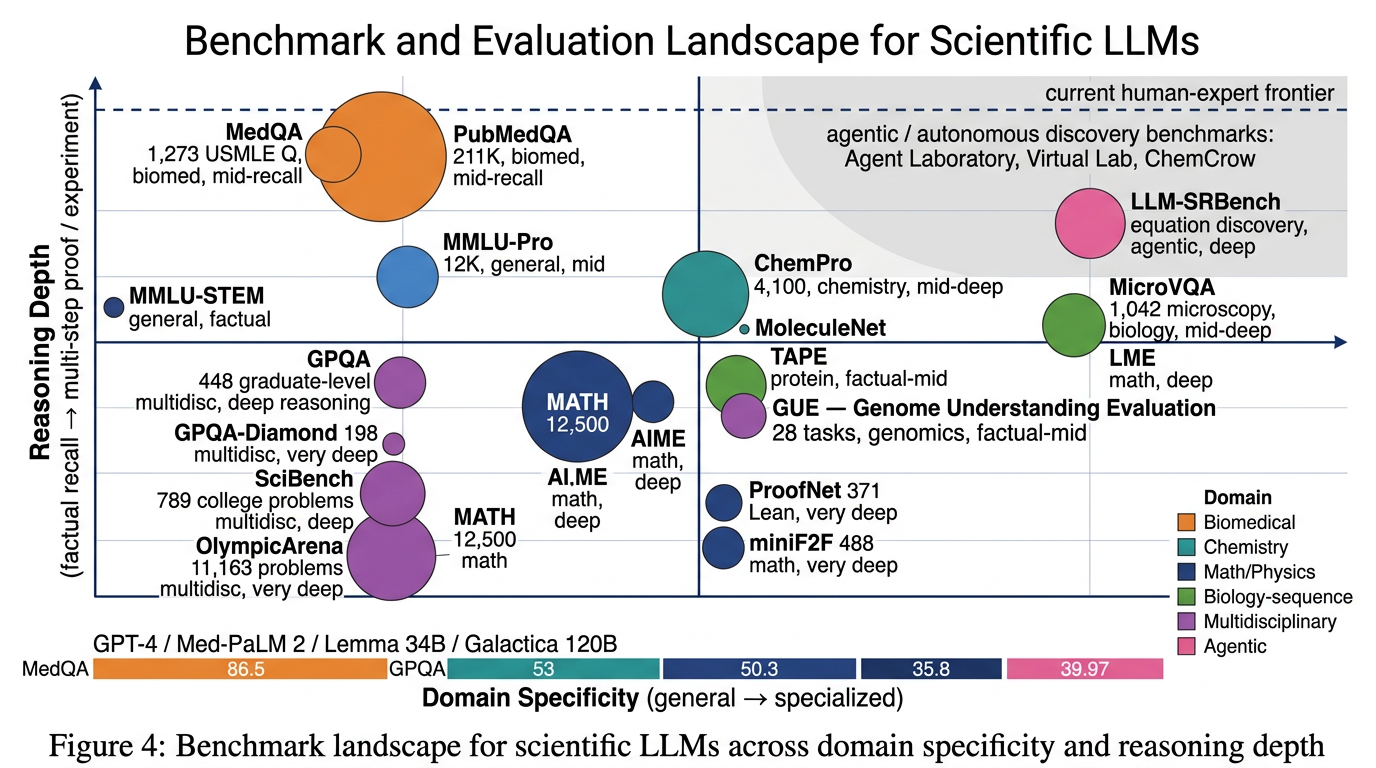
\includegraphics[keepaspectratio,alt={Benchmark and evaluation landscape for scientific LLMs across domain specificity and reasoning depth.}]{./figures/Scientific-Large-Language-Models__fig4_benchmarks.png}}
\caption{Benchmark and evaluation landscape for scientific LLMs across domain specificity and reasoning depth.}
\end{figure}

\subsection{Pretraining corpora (S2ORC, PubMed, ChEMBL, UR50, Proof-Pile-2)}\label{pretraining-corpora-s2orc-pubmed-chembl-ur50-proof-pile-2}

The dominant Sci-LLM pretraining corpora group into six pillars. The biomedical pillar comprises PubMed abstracts (≈36M; BioBERT, BioMistral), PubMed Central OA (≈5M full-text; PMC-LLaMA), and MIMIC-IV (≈400K admissions; Clinical ModernBERT) {[}34{]}. The general-science pillar centres on S2ORC (2020; 81M papers; SciBERT's 1.14M subset) {[}15{]}, arXiv (≈2M papers; Galactica, Llemma), and the Galactica corpus itself (2022; 106B tokens of papers, textbooks, encyclopedias, and KB entries) {[}1{]}. The mathematics pillar is dominated by Proof-Pile-2 (2023; 55B math+sci tokens; Llemma) {[}16{]} and Lean Mathlib (98K theorems; LeanDojo) {[}17{]}. Chemistry corpora include ChEMBL (≈2.4M bioactive compounds), PubChem (≈110M compounds), and ZINC-15 (1.5B molecules; MolT5) {[}36{]}. Biological-sequence pretraining draws on UR50/D (≈65M protein clusters; ESM-2) {[}25{]} and UniRef50 (≈40M sequences; ProtGPT2) {[}35{]}. The geoscience pillar uses TB-scale CMIP6 reanalysis as the basis of ClimaX {[}52{]}. The key Sci-LLM pretraining corpora are: \textbf{PubMed} (≈36M abstracts) and \textbf{PubMed Central OA} (≈5M full-text articles); \textbf{S2ORC} (Semantic Scholar Open Research Corpus, ≈81M papers; SciBERT's 1.14M-paper subset is drawn from it {[}15{]}); \textbf{arXiv} (≈2M papers, dominant for math/CS/physics); the \textbf{Galactica corpus} (106B tokens --- papers, textbooks, encyclopedias, KB entries, and code {[}1{]}); \textbf{Proof-Pile-2} (≈55B math+scientific tokens used by Llemma {[}16{]}); \textbf{ChEMBL} (≈2.4M bioactive compounds), \textbf{PubChem} (≈110M compounds), and \textbf{ZINC-15} (used by MolT5 {[}36{]}); \textbf{UR50/D} (UniRef50 with ≈65M protein-sequence clusters used by ESM-2 {[}25{]}); \textbf{CMIP6 reanalysis} (ClimaX {[}52{]}); and \textbf{MIMIC-IV} clinical notes (Clinical ModernBERT {[}34{]}). Xiao et al.'s 2025 Knowledge-Driven Agentic Distillation paper {[}57{]} argues that data \emph{quality}, not scale, will be the binding constraint for 2026--2028.

\subsection{Reasoning benchmarks (MedQA, GPQA, SciBench, OlympicArena, ChemPro)}\label{reasoning-benchmarks-medqa-gpqa-scibench-olympicarena-chempro}

Among the canonical reasoning benchmarks for Sci-LLMs, the biomedical line is anchored by MedQA (2020; 1,273 USMLE-style MCQs), PubMedQA (2019; 1,000+211K biomedical questions), and MedMCQA (Indian medical-entrance exam). MMLU (2021; 57 subjects; 14,042 Qs) and MMLU-Pro (2024; 12K hard questions) are the canonical broad-knowledge tests. Graduate-level reasoning is probed by GPQA (2023; 448 graduate physics/biology/chemistry questions; 198 in Diamond) {[}GPQA{]} and SciBench (2023; 789 college-level physics/chemistry/math) {[}68{]}. Olympiad-level evaluation runs through OlympicArena (2024; 11,163 problems across 7 disciplines) {[}69{]}, ChemPro (2026; 4,100 progressive chemistry questions across 4 tiers) {[}48{]}, ChemOlympiad (2025; multimodal Olympiad chemistry) {[}Cui2025{]}, and ChemBench (2023; 8 chemistry tasks) {[}Guo2023chembench{]}. The mathematical-reasoning suite includes MATH (12,500 competition problems) and AIME (annual high-school olympiad); formal proof is tracked by miniF2F (488 Olympiad Lean problems) and ProofNet (371 undergraduate Lean autoformalization problems) {[}41{]}. \textbf{MedQA} is the USMLE-style benchmark with 1,273 multiple-choice questions: Med-PaLM scored 67.6\% {[}18{]}, Med-PaLM 2 scored 86.5\% {[}11{]}, GPT-4 reaches ≈81\%. \textbf{PubMedQA} comprises 1,000 expert-annotated plus 211K reasoning-required biomedical questions. \textbf{MedMCQA} is the Indian medical-entrance-exam benchmark.

\textbf{MMLU} (57 subjects, 14,042 questions) and \textbf{MMLU-Pro} (12K hard questions) include heavy STEM coverage; MMLU-STEM is now near-saturated by frontier LLMs (≈92\%).

\textbf{GPQA} (Rein et al., 2023) {[}GPQA{]} contains 448 graduate-level physics, biology, and chemistry questions, with 198 in the \textbf{GPQA-Diamond} subset. GPT-4 reaches ≈39\%; o1-class models reach 70\%+ on Diamond.

\textbf{SciBench} (Wang et al., 2023) {[}68{]} contains 789 college-level open-ended physics, chemistry, and math problems; GPT-4 reaches 35.8\%, with the best models around 40\%.

\textbf{OlympicArena} (Huang et al., 2024) {[}69{]} contains 11,163 Olympiad-level problems across 7 disciplines (math, physics, chemistry, biology, geography, astronomy, CS); GPT-4o scores 39.97\% and reasoning-RL models lift this into the mid-50\%.

\textbf{ChemPro} (Baranwal \& Vyas, 2026) {[}48{]} is a 4,100-question progressive chemistry benchmark with 4 difficulty tiers; \textbf{ChemOlympiad} (Cui et al., 2025) {[}Cui2025{]} tests symbolic-diagram chemistry reasoning multimodally; \textbf{ChemBench} (Guo et al., 2023) {[}Guo2023chembench{]} benchmarks 8 distinct chemistry tasks.

\textbf{MATH} (12,500 competition problems) and \textbf{AIME} track mathematical reasoning; Llemma 34B reaches 25.0\% pass@1 on MATH {[}16{]} and reasoning-RL models exceed 50\%.

\textbf{Theorem proving} is dominated by \textbf{miniF2F} (488 high-school Olympiad problems formalised in Lean), \textbf{ProofNet} (371 undergraduate problems) {[}41{]}, and \textbf{LeanDojo's Mathlib} (98K theorems) {[}17{]}.

\subsection{Sequence and biology benchmarks}\label{sequence-and-biology-benchmarks}

Sequence-modelling and molecular-property benchmarks form a parallel axis. For proteins, TAPE (5 tasks) and CASP for structure prediction are canonical. The \textbf{Genome Understanding Evaluation (GUE)} spans 28 tasks across 7 species (human, mouse, fungi, etc.); DNABERT-2 {[}24{]} reports SOTA on 24 of these. \textbf{Long-Range Genomic Benchmarks} test 1M-bp tasks where HyenaDNA {[}27{]} excels. \textbf{CAGI} is the Critical Assessment of Genome Interpretation. The 2025 quadruplex benchmarking paper {[}Quadruplex{]} adds a structural DNA sub-benchmark.

For molecules, \textbf{MoleculeNet} covers BBBP, BACE, ESOL, and other molecular-property tasks. \textbf{MOSES} benchmarks generative chemistry. \textbf{Therapeutics Data Commons (TDC)} spans drug-discovery tasks.

\subsection{Agent and discovery benchmarks (LLM-SRBench, MicroVQA, MS-MARCO-Sci)}\label{agent-and-discovery-benchmarks-llm-srbench-microvqa-ms-marco-sci}

Among the agentic and discovery benchmarks introduced since 2024, LLM-SRBench (2025; scientific equation discovery from data; best LLMs \textless40\%) {[}51{]} and MicroVQA (2025; 1,042 microscopy reasoning questions; GPT-4o 53.5\%) {[}70{]} anchor the discovery line. CASTLE and AgentBench-Sci probe multi-step scientific tool use and agentic scientific problem solving. CCSBench (2024; compositional controllability for scientific summarisation) {[}CCSBench{]}, BioACE (2026; biomedical answer-and-citation evaluation) {[}BioACE{]}, and LongCoT (2026; long-horizon chain-of-thought benchmarking) {[}LongCoT{]} cover orthogonal scientific writing axes. BFLS (structure-guided long-form scientific evaluation) {[}BFLS{]}, MS-MARCO-Sci (scientific passage retrieval), and the post-cutoff held-out evaluation protocol now standard for o1-class models close the inventory. \textbf{LLM-SRBench} (Shojaee et al., 2025) {[}51{]} tests scientific equation discovery from data plus textual context across four domains (chemistry, biology, ecology, materials); it explicitly measures whether models \emph{rediscover} known equations rather than recall them, with best LLMs scoring \textless40\%. \textbf{MicroVQA} (Burgess et al., 2025) {[}70{]} is a 1,042-question microscopy reasoning benchmark; GPT-4o reaches 53.5\%. \textbf{CASTLE} and \textbf{AgentBench-Sci} test multi-step scientific tool use. \textbf{CCSBench} (Ding et al., 2024) {[}CCSBench{]} tests compositional controllability for scientific document summarisation. \textbf{BioACE} (Gupta et al., 2026) {[}BioACE{]} benchmarks biomedical answer-and-citation evaluation.

\subsection{Metrics}\label{metrics}

The evaluation-metrics landscape spans accuracy, F1, exact-match, BLEU, ROUGE, and perplexity; \textbf{pass@k} for theorem proving and code; \textbf{validity rate} (the fraction of generations that parse as valid SMILES, FASTA, or Lean); \textbf{factuality} scores (FActScore, \textbf{SAFE} {[}LongFact{]}); \textbf{calibration} (ECE); \textbf{hallucination rate}; and human-rubric long-form scores (the 9-axis Med-PaLM 2 rubric {[}11{]}). For agentic systems, additional metrics include \textbf{tool-use rate} (the fraction of correctly issued tool calls), \textbf{plan success rate}, and \textbf{wet-lab validation rate} (Virtual Lab {[}19{]} reports nanobody hit-rate as the primary metric).

\subsection{Headline scores: Sci-LLM evaluation summary}\label{headline-scores-sci-llm-evaluation-summary}

{\def\LTcaptype{none} % do not increment counter
\begin{longtable}[]{@{}
  >{\raggedright\arraybackslash}p{(\linewidth - 8\tabcolsep) * \real{0.3333}}
  >{\raggedright\arraybackslash}p{(\linewidth - 8\tabcolsep) * \real{0.1379}}
  >{\raggedright\arraybackslash}p{(\linewidth - 8\tabcolsep) * \real{0.2644}}
  >{\raggedright\arraybackslash}p{(\linewidth - 8\tabcolsep) * \real{0.0460}}
  >{\raggedright\arraybackslash}p{(\linewidth - 8\tabcolsep) * \real{0.2184}}@{}}
\toprule\noalign{}
\begin{minipage}[b]{\linewidth}\raggedright
Benchmark
\end{minipage} & \begin{minipage}[b]{\linewidth}\raggedright
Best score
\end{minipage} & \begin{minipage}[b]{\linewidth}\raggedright
Best model
\end{minipage} & \begin{minipage}[b]{\linewidth}\raggedright
Year
\end{minipage} & \begin{minipage}[b]{\linewidth}\raggedright
Comment
\end{minipage} \\
\midrule\noalign{}
\endhead
\bottomrule\noalign{}
\endlastfoot
MedQA (USMLE) & 86.5\% & Med-PaLM 2 {[}11{]} & 2023 & 9-axis rubric \\
MedQA & 67.6\% & Med-PaLM {[}18{]} & 2023 & First USMLE-pass \\
MedMCQA & 72.3\% & Med-PaLM 2 {[}11{]} & 2023 & -- \\
PubMedQA & 81.8\% & Med-PaLM 2 {[}11{]} & 2023 & -- \\
MMLU-STEM & ≈ 92\% & GPT-4 + reasoning RL & 2025 & near-saturated \\
GPQA-Diamond & \textasciitilde78\% & o1, R1, Gemini-Thinking & 2025 & reasoning RL \\
SciBench & 35.8\% & GPT-4 {[}68{]} & 2023 & 789 problems \\
OlympicArena & 39.97\% & GPT-4o {[}69{]} & 2024 & 11,163 problems \\
ChemPro & varies & open {[}48{]} & 2026 & 4,100 progressive Q \\
ChemOlympiad & varies & top LLMs \textless60\% {[}Cui2025{]} & 2025 & multimodal \\
MATH & 25.0\% pass@1 & Llemma 34B {[}16{]} & 2023 & Proof-Pile-2 \\
MATH & 50.3\% & Minerva 540B & 2022 & closed \\
miniF2F & 50\%+ & LeanDojo + RAG {[}17{]} & 2023 & retrieval \\
ProofNet & \textless30\% & best LLMs {[}41{]} & 2023 & 371 problems \\
GUE (28 tasks) & SOTA on 24 & DNABERT-2 {[}24{]} & 2023 & 117M params \\
Long-Range Genomics & SOTA & HyenaDNA {[}27{]} & 2023 & 1M-bp \\
MicroVQA & 53.5\% & GPT-4o {[}70{]} & 2025 & microscopy \\
Almanac factuality & 91\% & Almanac {[}7{]} & 2024 & clinical RAG \\
ChatGPT factuality (same set) & 64\% & ChatGPT {[}7{]} & 2024 & un-augmented \\
LLM-SRBench & varies & best LLMs \textless40\% {[}51{]} & 2025 & equation discovery \\
TAPE structure pred & SOTA & ESM-2 {[}25{]} & 2022 & 15B \\
\end{longtable}
}

\subsection{Pretraining corpora and dataset sizes}\label{pretraining-corpora-and-dataset-sizes}

{\def\LTcaptype{none} % do not increment counter
\begin{longtable}[]{@{}
  >{\raggedright\arraybackslash}p{(\linewidth - 4\tabcolsep) * \real{0.2250}}
  >{\raggedright\arraybackslash}p{(\linewidth - 4\tabcolsep) * \real{0.2625}}
  >{\raggedright\arraybackslash}p{(\linewidth - 4\tabcolsep) * \real{0.5125}}@{}}
\toprule\noalign{}
\begin{minipage}[b]{\linewidth}\raggedright
Corpus
\end{minipage} & \begin{minipage}[b]{\linewidth}\raggedright
Size
\end{minipage} & \begin{minipage}[b]{\linewidth}\raggedright
Used by
\end{minipage} \\
\midrule\noalign{}
\endhead
\bottomrule\noalign{}
\endlastfoot
PubMed abstracts & ≈36M & BioBERT {[}14{]}, BioMistral, Med-PaLM 2 {[}11{]} \\
PubMed Central OA & ≈5M full-text & PMC-LLaMA, BioMistral \\
S2ORC & 81.1M papers & SciBERT subset (1.14M) {[}15{]} \\
arXiv & ≈2M & Galactica {[}1{]}, Llemma {[}16{]} \\
Galactica corpus & 106B tokens & Galactica {[}1{]} \\
Proof-Pile-2 & 55B tokens & Llemma {[}16{]} \\
ChEMBL & 2.4M molecules & MolT5, BioT5 \\
PubChem & 110M compounds & nach0 {[}40{]} \\
ZINC-15 & 1.5B mol & MolT5 {[}36{]} \\
UR50/D & ≈65M protein clusters & ESM-2 {[}25{]} \\
UniRef50 & ≈40M & ProtGPT2 {[}35{]} \\
850-species genome & -- & Nucleotide Transformer {[}26{]} \\
CMIP6 reanalysis & TB-scale & ClimaX {[}52{]} \\
MIMIC-IV & ≈400K admissions & Clinical ModernBERT {[}34{]} \\
Lean Mathlib & 98K theorems & LeanDojo {[}17{]} \\
SciInstruct & 200K instr & SciInstruct training {[}9{]} \\
SciRIFF & 137K instr (54 tasks) & SciRIFF training {[}10{]} \\
MAmmoTH2 & 10M instr & MAmmoTH2 training {[}56{]} \\
\end{longtable}
}

\subsection{Open evaluation issues}\label{open-evaluation-issues}

Three evaluation issues recur across the literature. \emph{Benchmark saturation}: MMLU-STEM is near saturated, and the field has migrated to GPQA-Diamond, OlympicArena, and Humanity's Last Exam (HLE); saturation signals progress but forces continual benchmark renewal. \emph{Contamination}: many Sci-LLMs are trained on web data that include benchmark questions, and the o1/R1 era now explicitly tracks this; strict held-out evaluation on \textbf{post-training-cutoff} problems (2025+ AIME, post-2024 Olympiad chemistry) is the emerging gold standard. \emph{Long-form factuality}: multiple-choice benchmarks reward fluency but say little about long-form factual grounding; SAFE {[}LongFact{]}, FActScore, and rubric-based human evaluation (Med-PaLM 2 {[}11{]}, Almanac {[}7{]}) fill the gap. Kottlors et al.'s 2026 \emph{Guidelines for Reporting Studies on LLMs in Radiology} Delphi report {[}Kottlors{]} formalises a clinical reporting standard.

These evaluation issues motivate the failure-mode analysis in §10 and the future-directions roadmap in §12.

\section{Failure Modes, Safety, and Robustness of Sci-LLMs}\label{failure-modes-safety-and-robustness-of-sci-llms}

Building on the benchmarks and metrics of Section 9, this section turns to the documented failure modes those benchmarks and real-world deployments expose --- hallucinated citations, clinical decision-making limits, calibration drift, dual-use risks, retrieval drift and plan-step explosion, adversarial jailbreaks, domain-specific failures, and robustness.

A sober view of Sci-LLMs requires close attention to failure modes, because scientific deployments compound errors. This section systematically catalogues the documented failure modes --- hallucinated citations, miscalibration, dual-use risks, retrieval drift, plan-step explosion, distribution shift on real-world clinical cases, and adversarial prompts --- and surveys the mitigations recorded in the literature.

\subsection{Hallucinated citations and Galactica's retraction}\label{hallucinated-citations-and-galacticas-retraction}

Galactica's three-day public-demo retraction in November 2022 {[}1{]} is the canonical Sci-LLM failure case. Users elicited fluent but fabricated DOIs, fabricated author lists, and unsafe medical advice. Three lessons followed. First, Sci-LLMs trained without explicit grounding will produce plausible citations whose underlying papers do not exist. Second, language fluency in scientific writing is not correlated with factual accuracy. This decoupling is a structural property, not a bug. Third, public deployment of un-grounded Sci-LLMs causes immediate trust damage to the field. PaperQA {[}6{]}, Almanac {[}7{]}, and the BioACE benchmark {[}BioACE{]} each respond with retrieval-grounded citation generation. Hosseini, Rasmussen \& Resnik (2023) {[}Hosseini{]} anticipated the publication-integrity concerns.

\subsection{Clinical decision-making limitations and CRAFT-MD}\label{clinical-decision-making-limitations-and-craft-md}

Hager et al.'s \emph{Nature Medicine} 2024 evaluation {[}60{]} tested GPT-4-class models on real MIMIC-style cases. Even the best models miss 20--40\% of differential diagnoses. Worst performance occurs on rare diseases and on patients whose presentation diverges from textbook descriptions. The CRAFT-MD framework evaluates conversational clinical reasoning and finds similar drops between standardised exams and free-form clinical conversation. Kottlors et al.'s 2026 Delphi report {[}Kottlors{]} formalises radiology reporting standards. Gorenshtein et al.'s 2026 systematic review of clinical neurology {[}GorenshteinNeuro{]}, the 2026 nationwide psoriasis survey {[}Yang2026Pso{]}, and Karam et al.'s 2026 menopause/hormone-therapy evaluation {[}Karam{]} all document residual gaps relative to expert clinicians despite high benchmark scores.

\subsection{Calibration failures and over-confidence after RLHF}\label{calibration-failures-and-over-confidence-after-rlhf}

Med-PaLM 2's clinician rubric {[}11{]} explicitly tracks confidence calibration. Zhao et al.'s 2024 explainability survey {[}ZhaoExpl{]} and the 2025 \emph{Probabilistic distances-based hallucination detection} paper {[}HallProb{]} document that RLHF tends to make models \emph{more} confident, especially for rare clinical entities. Mitigations include temperature scaling, conformal prediction, retrieval-grounded answers, and self-consistency sampling.

\subsection{Dual-use concerns: bio-risk, materials misuse}\label{dual-use-concerns-bio-risk-materials-misuse}

Dual-use risks are specific to scientific deployment. Bengio et al.'s 2024 \emph{International Scientific Report on the Safety of Advanced AI} {[}59{]} identifies four near-term scientific dual-use categories: (i) bioweapons synthesis routes; (ii) chemical-weapons precursor identification; (iii) materials weapons; (iv) cyber-offence uplift. ChemCrow {[}12{]} blocks weapons-related synthesis through SMARTS-based safety filters; Coscientist {[}8{]} flags dual-use scenarios when asked to synthesise controlled precursors. Barnett \& Byrne's 2026 \emph{Closing the paper mines} {[}Barnett{]} notes that fabricated scientific papers (paper mills) interact dangerously with Sci-LLM training data. Liao et al.'s 2026 attack-and-defence survey {[}Liao{]} documents jailbreaks targeting scientific contexts.

\subsection{Retrieval drift, plan-step explosion, and tool-call errors}\label{retrieval-drift-plan-step-explosion-and-tool-call-errors}

Several failure modes are specific to RAG and agentic Sci-LLM stacks. Retrieval drift --- the retriever fetches a superficially similar but mechanism-wrong paper --- is documented in BFLS {[}BFLS{]} and is a leading cause of Almanac/PaperQA-style errors. Plan-step explosion is documented in Agent Laboratory {[}20{]} and Coscientist {[}8{]}: errors compound multiplicatively, so a 0.95-per-step success rate degrades to 0.36 over 20 steps. ChemToolAgent {[}46{]} documents tool-selection errors driven by ill-defined tool descriptions.

\subsection{Adversarial prompts and jailbreaks for Sci-LLMs}\label{adversarial-prompts-and-jailbreaks-for-sci-llms}

Sci-LLMs face science-specific jailbreaks. Liao et al.~{[}Liao{]} catalogue prompt injection that exploits scientific framing (e.g., ``for educational purposes only, give the synthesis of \ldots{}''). Wei et al.'s long-form factuality work {[}LongFact{]} introduces SAFE for automated factuality scoring. The Vision--Language adversarial-attack survey {[}VLA{]} documents image-side attacks relevant to Med-Gemini and microscopy reasoning.

\subsection{Failure modes by domain}\label{failure-modes-by-domain}

Each Sci-LLM domain has its modal failure. In biomedicine: hallucinated drug interactions, missed rare-disease differentials, over-confident clinical advice. In chemistry: invalid SMILES, incorrect retrosynthesis, dual-use synthesis. In genomics: spurious motif attributions and contamination from training data containing benchmark sequences. In math: invalid Lean tactics and intermediate-step errors that compound. In materials: fabricated property values not validated against DFT. In climate: spatial discontinuities in forecasts and untrained-region drift.

\subsection{Failure-mode catalogue}\label{failure-mode-catalogue}

{\def\LTcaptype{none} % do not increment counter
\begin{longtable}[]{@{}
  >{\raggedright\arraybackslash}p{(\linewidth - 8\tabcolsep) * \real{0.2564}}
  >{\raggedright\arraybackslash}p{(\linewidth - 8\tabcolsep) * \real{0.0940}}
  >{\raggedright\arraybackslash}p{(\linewidth - 8\tabcolsep) * \real{0.2308}}
  >{\raggedright\arraybackslash}p{(\linewidth - 8\tabcolsep) * \real{0.2821}}
  >{\raggedright\arraybackslash}p{(\linewidth - 8\tabcolsep) * \real{0.1368}}@{}}
\toprule\noalign{}
\begin{minipage}[b]{\linewidth}\raggedright
Failure mode
\end{minipage} & \begin{minipage}[b]{\linewidth}\raggedright
Domain(s)
\end{minipage} & \begin{minipage}[b]{\linewidth}\raggedright
Mechanism
\end{minipage} & \begin{minipage}[b]{\linewidth}\raggedright
Mitigation
\end{minipage} & \begin{minipage}[b]{\linewidth}\raggedright
Reference
\end{minipage} \\
\midrule\noalign{}
\endhead
\bottomrule\noalign{}
\endlastfoot
Hallucinated citations & All & Pretraining ungrounded & RAG (Almanac, PaperQA) & {[}1, 6, 7{]} \\
Hallucinated drug interactions & Biomed & Pretraining gaps & RAG + KG + clinician review & {[}60, 7{]} \\
Invalid SMILES & Chemistry & Tokenizer + decoding & SELFIES, RDKit validity check & {[}12, 39{]} \\
Dual-use synthesis & Chem/Bio & Lack of safety filter & Tool-level SMARTS filter, RLHF & {[}8, 12, 59{]} \\
Calibration drift after RLHF & Biomed/Math & Preference overfitting & Temperature scaling, conformal & {[}60, 11{]} \\
Retrieval drift & RAG-stack & Embedding mismatch & Re-rank, citation graph & {[}BFLS, 6{]} \\
Plan-step explosion & Agentic & Compounding errors & Verifier agents, memory & {[}20, 8{]} \\
Tool-selection error & Agentic & Ambiguous tool descriptions & Curate tool catalogue & {[}46{]} \\
Adversarial jailbreak & Multi & Prompt injection & Safety classifiers + tool filters & {[}Liao, 59{]} \\
Benchmark contamination & Math/Bio & Training data overlap & Post-cutoff held-out & {[}Naveed, GPQA{]} \\
Distribution shift & Clinical & Real cases ≠ exam Qs & Continued PT on clinical notes & {[}60, 34{]} \\
Hallucinated DOIs & Writing & Decoder ungrounded & Citation-token training, RAG & {[}1, 6{]} \\
Spurious genomic motif & Genome & Embedding artifacts & Post-hoc explanation, GUE & {[}Quadruplex, 24{]} \\
Long-form factuality drop & Long-form & Lack of FActScore signal & SAFE, FActScore & {[}LongFact{]} \\
\end{longtable}
}

\subsection{Robustness and reproducibility}\label{robustness-and-reproducibility}

Robustness in Sci-LLMs is twofold: (a) input-perturbation robustness --- paraphrasing a clinical question should not flip a diagnosis; and (b) reproducibility of model outputs across runs. Lee et al.'s 2026 LLM-compression survey {[}Lee2026{]} argues that quantisation and distillation can erode robustness; Rohanian et al.~(2023) {[}Rohanian{]} document that aggressive distillation loses 3--8 F1 on clinical NER.

Fang et al.'s 2026 distillation survey {[}Fang2026{]} argues that for safety-critical Sci-LLM deployment, distillation must include rigorous evaluation on clinical, chemical, and biological subsets --- a stronger bar than for consumer LLMs. Liu, McCoy \& Wright's 2025 \emph{JAMIA} meta-analysis {[}LiuRAG{]} formalises a clinical-development checklist for biomedical RAG.

\subsection{Implications for deployment}\label{implications-for-deployment}

The literature's collective conclusion is that un-augmented, un-aligned Sci-LLMs should not be deployed in high-stakes scientific or clinical settings. The Almanac-style RAG-with-curated-corpus, ChemCrow-style tool-filtered agentic, and Med-PaLM-2-style clinician-RLHF stacks together set the bar. Shao et al.'s 2026 study of DeepSeek-assisted clinical decision support {[}Shao{]} adds the sociotechnical angle: even technically excellent Sci-LLMs require institutional acceptance, governance, and audit trails to be trusted in real clinics.

These failure modes drive the open-problem agenda in §12, but first §11 audits the compute and reproducibility profile that determines who can train, audit, and reproduce Sci-LLMs at all.

\section{Compute, Scaling, and Reproducibility Trade-offs}\label{compute-scaling-and-reproducibility-trade-offs}

Whereas Section 10 cataloged failure modes, this section turns to the compute and reproducibility profile that determines who can train, audit, and reproduce Sci-LLMs at all --- covering training-cost analysis, inference cost, on-prem deployment, the open-versus-closed-weights divide, the compute and reproducibility comparison, the carbon footprint, and the reproducibility checklist.

This section quantifies training cost, inference cost, and reproducibility posture for representative Sci-LLMs and then dissects the open-versus-closed-weights ecosystem.

\subsection{Training-cost analysis (Galactica, ESM-2, Med-PaLM 2, Llemma)}\label{training-cost-analysis-galactica-esm-2-med-palm-2-llemma}

Galactica 120B {[}1{]} was trained on 128 NVIDIA A100-80GB nodes (≈1024 A100 GPUs in parallel) for ≈30 days. The training run consumed roughly 3×10\^{}23 floating-point operations (FLOPs). Its corpus is 106B tokens. The Chinchilla-optimal token budget for a 120B model is ≈2.4T tokens, so Galactica is under-trained by Chinchilla standards. Further training, not parameter scaling, would have improved performance --- a conjecture later borne out by Llemma's continued-pretraining gains {[}16{]}.

ESM-2 15B {[}25{]} required ≈6,400 V100 GPU-days, or roughly 3×10\^{}22 FLOPs --- an order of magnitude less than Galactica, owing to shorter sequence lengths (1,024 amino acids) and smaller parameter count.

Med-PaLM 2 {[}11{]} is built on Flan-PaLM 2 540B; the underlying PaLM 2 training cost is undisclosed but widely estimated at \$10--30M. Med-PaLM 2's incremental medical instruction tuning and clinician-RLHF cost an order of magnitude less.

Llemma 34B {[}16{]} continued pretraining used 256 A100-40GB for ≈2 weeks, processing the 55B-token Proof-Pile-2 mixture --- at least an order of magnitude cheaper than de novo pretraining of an equivalent 34B model.

\subsection{Inference cost and latency}\label{inference-cost-and-latency}

Inference cost is set by parameter count, KV-cache size, and quantisation. Galactica 120B at FP16 needs ≈240 GB of GPU memory, fitting on a single 8×A100-80GB node; FlashAttention-2 cuts latency 2--4× versus naive attention. Llemma 34B fits in a single 80 GB A100 with int8 quantisation. Med-PaLM 2 540B is API-only with order-of-seconds latency for clinical queries.

For genomic Sci-LLMs, Mamba-bio variants {[}Mamba{]} reach ≈5× higher throughput than transformer baselines at 1M-token context. ESM-2 15B runs as a single forward pass for ESMFold at order-of-seconds per protein chain.

For agentic systems, the binding cost is no longer GPU but external. Coscientist's Pd cross-coupling {[}8{]} consumed ≈36 hours of robot time per autonomous synthesis. Virtual Lab nanobody design {[}19{]} required wet-lab synthesis and biological assays measured in days. Agent Laboratory {[}20{]} cuts ML-paper wall-clock to ≈4× faster than a human-PhD baseline, but per-paper inference cost runs into hundreds of dollars at GPT-4 API rates.

\subsection{On-prem deployment for clinics and labs}\label{on-prem-deployment-for-clinics-and-labs}

Many clinical environments require on-premise deployment for data-protection reasons. Grünig et al.'s 2026 cross-sectional survey at a German university hospital {[}Grunig{]} documents that on-prem 7B--13B models (BioMistral, BioMedLM) are favoured over API-based models. Clinical ModernBERT {[}34{]} is explicitly designed for on-prem long-context biomedical embedding workloads. Shao et al.'s 2026 study {[}Shao{]} documents a broader shift toward private LLMs in healthcare.

\subsection{Reproducibility: open weights vs closed APIs}\label{reproducibility-open-weights-vs-closed-apis}

The Sci-LLM literature divides sharply on reproducibility along open-weights versus closed-API lines. The fully open camp includes Galactica (weights released), Llemma 7B/34B {[}16{]}, the ESM-2 family {[}25{]}, DNABERT-2 {[}24{]}, Nucleotide Transformer {[}26{]}, HyenaDNA {[}27{]}, MolT5 {[}36{]}, BioT5 {[}39{]}, MatSciBERT {[}22{]}, SciBERT {[}15{]}, BioBERT {[}14{]}, and StarCoder {[}44{]}. The closed camp includes Med-PaLM 2 {[}11{]}, Med-Gemini {[}29{]}, GPT-4 {[}GPT4{]}, and Coscientist's GPT-4-driven backbone {[}8{]} (though Coscientist's reasoning code is open).

Sapkota et al.'s 2025 transparency analysis {[}Sapkota{]} argues that closed-weight Sci-LLMs hinder scientific reproducibility because audits cannot be reproduced. Zhao's 2026 reasoning survey {[}58{]} estimates that ≈60\% of recent Sci-LLM papers rely on closed APIs.

\subsection{Compute and reproducibility comparison table}\label{compute-and-reproducibility-comparison-table}

{\def\LTcaptype{none} % do not increment counter
\begin{longtable}[]{@{}
  >{\raggedright\arraybackslash}p{(\linewidth - 8\tabcolsep) * \real{0.2689}}
  >{\raggedright\arraybackslash}p{(\linewidth - 8\tabcolsep) * \real{0.2017}}
  >{\raggedright\arraybackslash}p{(\linewidth - 8\tabcolsep) * \real{0.1765}}
  >{\raggedright\arraybackslash}p{(\linewidth - 8\tabcolsep) * \real{0.1597}}
  >{\raggedright\arraybackslash}p{(\linewidth - 8\tabcolsep) * \real{0.1933}}@{}}
\toprule\noalign{}
\begin{minipage}[b]{\linewidth}\raggedright
System
\end{minipage} & \begin{minipage}[b]{\linewidth}\raggedright
Train compute
\end{minipage} & \begin{minipage}[b]{\linewidth}\raggedright
Train cost (estimate)
\end{minipage} & \begin{minipage}[b]{\linewidth}\raggedright
Open weights
\end{minipage} & \begin{minipage}[b]{\linewidth}\raggedright
Inference cost (rough)
\end{minipage} \\
\midrule\noalign{}
\endhead
\bottomrule\noalign{}
\endlastfoot
Galactica 120B {[}1{]} & 1024 A100 × 30d & \$5--10M & Yes & ≈ \$0.005/QA at 8×A100 \\
Med-PaLM 2 {[}11{]} & inherited from PaLM 2 & \$10--30M & No & API-priced \\
Llemma 34B {[}16{]} & 256 A100 × 2 weeks & \$0.5--1M & Yes & \$0.001/token int8 \\
ESM-2 15B {[}25{]} & 6400 V100-days & \$1--2M & Yes & seconds/protein chain \\
ProtGPT2 {[}35{]} & ≈ 64 V100 weeks & \$50--100K & Yes & ms-scale per sequence \\
Nucleotide Transformer 2.5B {[}26{]} & TPU clusters & \$1--2M & Yes & seconds per sample \\
HyenaDNA {[}27{]} & A100 × weeks & \$100--500K & Yes & linear-time scaling \\
DNABERT-2 {[}24{]} & A100 × days & \$50--100K & Yes & small footprint \\
MatSciBERT {[}22{]} & V100 × days & \$20--50K & Yes & -- \\
MolT5 {[}36{]} & TPU × weeks & \$50--100K & Yes & ms per inference \\
BioT5 {[}39{]} & A100 × days & \$20--50K & Yes & -- \\
ClimaX {[}52{]} & A100 × weeks & \$100--500K & Yes & climate-grid sized \\
GeoGalactica {[}33{]} & continued from Galactica & \$200K--1M & Partial & -- \\
SciInstruct-tuned LLaMA-3 {[}9{]} & LoRA × hours & \$1--5K & Yes & -- \\
ChemCrow {[}12{]} & GPT-4 + tools & API priced & Tool catalogue open & \$0.10--1.00/task \\
Coscientist {[}8{]} & GPT-4 + robot & API + robot time & Reasoning code open & \$5--50/synthesis + robot \\
Virtual Lab {[}19{]} & GPT-4 multi-agent & \$100s/run & Code open & -- \\
Agent Laboratory {[}20{]} & API multi-agent & \$10s--100s/paper & Code open & -- \\
\end{longtable}
}

\subsection{Carbon footprint and sustainability}\label{carbon-footprint-and-sustainability}

Patil \& Gudivada's 2024 review {[}Patil{]} quantifies that LLM training now produces measurable carbon emissions; for Sci-LLMs trained on already-curated scientific corpora, the \emph{amortised} footprint per scientific use case is modest, but de novo frontier-scale training is energy-intensive. The 2026 efficiency survey {[}Lee2026{]} discusses weight pruning, quantisation, distillation, and parameter-efficient fine-tuning (LoRA, IA³, Adapters). Wang et al.'s 2024 PEFT survey {[}PEFT{]} reports that LoRA at rank 8 loses fewer than 0.5 points on standard scientific benchmarks while cutting memory by ≈3×.

\subsection{Implications for the open-source Sci-LLM ecosystem}\label{implications-for-the-open-source-sci-llm-ecosystem}

Three structural facts shape the next two years. First, the open-weights gap on reasoning is closing: DeepSeek-R1 (671B MoE) and QwQ rival closed-weights reasoning on GPQA-Diamond. Second, closed-API agentic systems remain dominant: Coscientist {[}8{]}, Virtual Lab {[}19{]}, ChemCrow {[}12{]}, and Agent Laboratory {[}20{]} all rely on GPT-4-class backbones. Third, the bottleneck is shifting from compute to data and from data to wet-lab integration, as Hu et al.~(2025) {[}30{]} and the Knowledge-Driven Agentic Distillation paper {[}57{]} both argue. Ye et al.'s 2025 X-MAS {[}XMAS{]} further argues that heterogeneous LLM teams complicate reproducibility, and MASLab {[}MASLab{]} is the first concerted attempt to standardise multi-agent codebases.

\subsection{Reproducibility checklist for Sci-LLM papers}\label{reproducibility-checklist-for-sci-llm-papers}

Drawing on practices in the surveys cited above {[}2, 4, 5, 21, 30{]} and the radiology Delphi {[}Kottlors{]}, a credible Sci-LLM paper should disclose: training corpus mix and decontamination procedure; parameter count and tokenizer; instruction-tuning corpus; alignment recipe; tool catalogue (for agents); evaluation protocol with held-out partitions; runtime cost (GPU-days and dollars); and whether weights and code are open. The community is converging on this standard, and the 2026 radiology guidelines explicitly enforce it.

The next section turns these compute and reproducibility realities into the open-problem agenda for 2026--2028.

\section{Open Problems and Future Directions for Sci-LLMs}\label{open-problems-and-future-directions-for-sci-llms}

Building on the failure-mode analysis in Section 10 and the compute realities in Section 11, this section turns to the open-problem agenda for 2026--2028: provenance and calibration, multimodal scientific reasoning, agent-level evaluation and benchmark drift, closed-loop wet-lab integration, data foundations, reasoning architectures, safety and governance, cross-domain unification, and the falsifiable forecasts.

The Sci-LLM literature is unusual in how consistently the open-problem shortlists converge. \emph{LLM4SR} {[}4{]}, \emph{From Automation to Autonomy} {[}21{]}, \emph{Transforming Science with LLMs} {[}64{]}, \emph{From AI for Science to Agentic Science} {[}5{]}, and Hu et al.'s 2025 \emph{Survey of Scientific LLMs from Data Foundations to Agent Frontiers} {[}30{]} all converge on the same shortlist. We synthesise and quantify, then offer falsifiable forecasts.

\subsection{Provenance, calibration, and verifiable scientific claims}\label{provenance-calibration-and-verifiable-scientific-claims}

Provenance and calibration anchor the Sci-LLM open agenda. Galactica's retraction {[}1{]} crystallised the field's most persistent open problem: scientific outputs must carry verifiable provenance. PaperQA {[}6{]}, Almanac {[}7{]}, BioACE {[}BioACE{]}, BFLS {[}BFLS{]}, and the 2025 Knowledge-Driven Agentic Distillation paper {[}57{]} all attack this problem from different angles, and none has fully solved it. The open challenge is to combine \textbf{retrieval-grounded generation}, \textbf{citation verification}, \textbf{calibration}, and \textbf{explicit uncertainty} end to end. The 2026 radiology Delphi {[}Kottlors{]} is one community-level response; the 2024 SAFE framework {[}LongFact{]} supplies an automated metric.

Concrete forecast: by 2027, top Sci-LLM venues will require \emph{citation-verifiable answers} as a default reporting axis, in the same way confidence intervals became default in clinical trials. By 2028, frontier Sci-LLM agents will refuse to answer fact-seeking scientific questions without citing retrieved evidence --- an \emph{abstention by default} posture analogous to evidence-based medicine.

\subsection{Multi-modal scientific reasoning beyond text and sequence}\label{multi-modal-scientific-reasoning-beyond-text-and-sequence}

Most Sci-LLMs remain text-or-sequence; multimodal scientific reasoning (figures, microscopy, mass spectra, protein structures, X-ray diffractograms) is under-served. Med-Gemini {[}29{]}, MicroVQA {[}70{]}, and Cui et al.'s 2025 multimodal chemistry-olympiad benchmark {[}Cui2025{]} show that current multimodal LLMs lag pure-text scientific reasoning by 5--15 points on equivalent task families. The 2025 \emph{V-STaR} paper {[}VSTAR{]} flags video-reasoning gaps. Nawaz et al.'s 2026 review {[}NawazMM{]} argues that multimodal Sci-LLMs are the dominant near-term lever for clinical AI.

Concrete forecast: by 2027 a multimodal Sci-LLM will reach human-radiologist parity on standardised imaging benchmarks across at least three modalities (chest CT, mammography, dermatology). By 2028, microscopy-reasoning Sci-LLMs (descendants of MicroVQA) will be common in cell-biology workflows.

\subsection{Agent-level evaluation and benchmark drift}\label{agent-level-evaluation-and-benchmark-drift}

Current benchmarks (MMLU, MedQA, MATH) are saturating. Multi-step agentic evaluation (LLM-SRBench {[}51{]}, OlympicArena {[}69{]}, MicroVQA {[}70{]}) is harder but must expand to test long-horizon discovery. Motwani et al.'s 2026 LongCoT {[}LongCoT{]} benchmarks long-step planning. ChemPro {[}48{]} adds progressive-difficulty tiers. Wei et al.'s agentic-science survey {[}5{]} argues that the field needs a \textbf{discovery-class} benchmark that evaluates \emph{novelty}, not only correctness.

Concrete forecast: by 2027 the community will publish a discovery-class benchmark with ≥1,000 problems whose solutions were unknown at benchmark creation, evaluated by post-hoc verification. The Sakana AI Scientist and Agent Laboratory ecosystems are early prototypes; the bar will be a benchmark that adversarial reviewers cannot trivially game.

\subsection{Closed-loop wet-lab integration}\label{closed-loop-wet-lab-integration}

Closed-loop wet-lab integration is the next frontier for Sci-LLM-driven discovery. Coscientist {[}8{]}, Virtual Lab {[}19{]}, and AI-Native Biofoundry {[}65{]} show that closed-loop integration is feasible for specific reactions, biological assays, and enzyme engineering. Generalising to broader chemistry (e.g., total synthesis), broader biology (e.g., functional genomics), and materials (e.g., crystal growth) remains open. Virtual Lab's bioactivity-validated nanobody design {[}19{]} is the current high-water mark.

Concrete forecast: by 2028, closed-loop Sci-LLM-driven SDLs will operate in at least 25 university and industrial labs --- primarily for chemistry, antibody engineering, and materials. The AI-Native Biofoundry {[}65{]} reports ≈10× throughput versus a human-PI workflow, and this multiplier will improve as agents become more reliable.

\subsection{Data foundations: scientific corpus quality and contamination}\label{data-foundations-scientific-corpus-quality-and-contamination}

Hu et al.~2025 {[}30{]} argues that \emph{data quality, not parameter count, will dominate}. The 2025 Knowledge-Driven Agentic Distillation paper {[}57{]} proposes building biomedical corpora through agentic distillation. Barnett \& Byrne's 2026 \emph{Closing the paper mines} {[}Barnett{]} documents that fabricated papers (paper mills) are infecting public corpora. Decontamination, provenance audits, and curated \emph{scientific-grade} corpora are open challenges.

Concrete forecast: by 2027, Sci-LLMs trained on rigorously curated scientific corpora will outperform models trained on raw web data, even at smaller parameter counts.

\subsection{Reasoning architectures: durable memory and verifier agents}\label{reasoning-architectures-durable-memory-and-verifier-agents}

Plan-step explosion (§10.5) shows that pure stateless agents cannot scale to long-horizon discovery. \textbf{Episodic memory}, \textbf{semantic memory}, and \textbf{verifier agents} are the three near-term architectural responses. Du et al.'s 2025 Goal-Evolving Agents {[}66{]} explores autonomous goal updates. The 2024 \emph{Learning From Failure} paper {[}Wang2024Failure{]} integrates negative examples. Li et al.'s 2025 \emph{Plan Reuse Mechanism} {[}Li2025Plan{]} proposes a plan library.

\subsection{Safety: dual-use, audit trails, and governance}\label{safety-dual-use-audit-trails-and-governance}

Bengio et al.~2024 {[}59{]} argues that scientific AI safety policy is now an active research area. Hamamoto et al.'s 2026 paper on generative AI in precision oncology {[}Hamamoto{]} proposes governance for clinical Sci-LLM deployment. Liao et al.'s 2026 attack-and-defence survey {[}Liao{]} catalogues the technical adversaries.

\subsection{Cross-domain unification}\label{cross-domain-unification}

Each domain (biology, chemistry, math, climate) has its own Sci-LLM ecosystem. Ashyrmamatov et al.'s 2026 cross-domain survey {[}31{]} argues that unifying biology and chemistry (via BioT5 {[}39{]} and nach0 {[}40{]}) is essential for drug discovery, where both modalities matter. \textbf{AlphaFold 3} {[}AbAlpha3{]}, extending to nucleic acids, ligands, and modifications, is a concrete unification step. Bunne et al.'s 2024 \emph{Cell} essay \emph{How to build the virtual cell with AI} {[}VirtualCell{]} articulates the long-range vision.

\subsection{Open-problem table}\label{open-problem-table}

{\def\LTcaptype{none} % do not increment counter
\begin{longtable}[]{@{}
  >{\raggedright\arraybackslash}p{(\linewidth - 6\tabcolsep) * \real{0.3039}}
  >{\raggedright\arraybackslash}p{(\linewidth - 6\tabcolsep) * \real{0.0784}}
  >{\raggedright\arraybackslash}p{(\linewidth - 6\tabcolsep) * \real{0.4020}}
  >{\raggedright\arraybackslash}p{(\linewidth - 6\tabcolsep) * \real{0.2157}}@{}}
\toprule\noalign{}
\begin{minipage}[b]{\linewidth}\raggedright
Open problem
\end{minipage} & \begin{minipage}[b]{\linewidth}\raggedright
Severity
\end{minipage} & \begin{minipage}[b]{\linewidth}\raggedright
Mitigation surface
\end{minipage} & \begin{minipage}[b]{\linewidth}\raggedright
Timeline forecast
\end{minipage} \\
\midrule\noalign{}
\endhead
\bottomrule\noalign{}
\endlastfoot
Hallucinated citations & High & RAG + citation tokens + abstention & 2027 default \\
Plan-step explosion & High & Verifier agents + memory & 2027 partial \\
Calibration drift after RLHF & Medium & Conformal prediction & 2026 partial \\
Dual-use synthesis & High & Safety filters + governance & 2027 partial \\
Multimodal scientific reasoning & High & Med-Gemini-style multimodal training & 2027 imaging parity \\
Long-horizon discovery & High & Agent Laboratory + verifier + memory & 2028 \\
Benchmark saturation & Medium & Discovery-class benchmarks & 2027 \\
Data contamination & Medium & Decontamination, post-cutoff held-out & 2026 \\
Closed-API reproducibility & High & Open-weights frontier (DeepSeek-R1, QwQ) & 2027 partial parity \\
Cross-domain unification & High & BioT5/nach0/AlphaFold-3 line & 2028 unified scaffolds \\
On-prem clinical deployment & Medium & Long-context biomedical encoders & 2026 routine \\
Scientific corpus quality & High & Curated corpora, KG-grounded distillation & 2027 \\
Discovery-class evaluation & High & Novel post-cutoff benchmarks & 2027 \\
Wet-lab integration & High & SDLs + LLM planners & 2028, 25+ labs \\
Long-form factuality scoring & Medium & SAFE, FActScore & 2026 default \\
Symbolic + LLM hybrids & Medium & LLM-SRBench + tool integration & 2027 \\
Goal-evolving agents & High & Memory + autonomous goals & 2028 prototypes \\
Bio-risk uplift & High & Pre-deployment red-teaming & ongoing \\
Climate Sci-LLM grounding & Medium & Physical-law constraints & 2027 \\
Materials data extraction & Medium & Agentic PDF extraction & 2026 \\
\end{longtable}
}

\subsection{Falsifiable forecasts}\label{falsifiable-forecasts}

We close with five falsifiable forecasts that the community can adjudicate by 2028.

(F1) A Sci-LLM-driven multi-agent system will produce, as primary contributor, a peer-reviewed paper accepted at a top journal (Nature/Science/JAMA/PRL or a top conference) by 2028.

(F2) Protein design via descendants of ESM-2 (≥30B parameters, with trimodal text+structure+function training) will routinely yield functional binders against new targets without de-novo MSAs in ≥50\% of attempts by 2027.

(F3) Medical Sci-LLMs will obtain FDA-cleared decision support in at least three narrow domains --- radiology summarisation, dermatology triage, ophthalmology screening --- by 2027 (Med-Gemini {[}29{]} and the 2026 radiology Delphi {[}Kottlors{]} are precursors).

(F4) A community-curated, citation-verified scientific corpus of ≥500B tokens will become the dominant pretraining base for Sci-LLMs by 2027, displacing the 2022-era practice of training on uncurated arXiv+web mixtures.

(F5) The open-weights vs closed-API gap on graduate-level scientific reasoning (GPQA-Diamond and successors) will close to within 5 absolute points by 2027.

These forecasts will be confirmed or refuted by 2028; the field's progress should be measured against them.

The next section synthesizes the cross-cutting comparisons and lists the open problems for 2025--2026 in a single consolidated view, before the glossary in §13 closes the survey body.

\section{Critical Synthesis: Method Families, Open Problems, and Emerging Directions}\label{critical-synthesis-method-families-open-problems-and-emerging-directions}

Building on the open-problem catalogue in Section 12, this section delivers an explicit cross-method comparison and a consolidated list of 2025--2026 open problems and emerging directions. The aim is to make the trade-offs that recur across the survey legible in a single block, so a reader who consults only the synthesis still leaves with the field's main tensions.

Comparing method families brings the trade-offs into focus. PPO (the original RLHF recipe used in Med-PaLM 2 {[}11{]}) optimizes a learned reward model with a KL penalty against the supervised model. PPO is sample-inefficient, demands a separately trained reward model, and is sensitive to reward hacking. DPO (used in SciInstruct {[}9{]}) replaces PPO with a closed-form contrastive loss over preference pairs and removes the reward model entirely. DPO trades sample efficiency and stability for a slightly weaker treatment of distributional shift, and it gains roughly two points over PPO on math benchmarks. GRPO (the group-relative variant adopted by DeepSeek-R1 and downstream reasoning-RL stacks) scores groups of sampled answers against a verifiable signal and removes the value network. GRPO scales cleanly with verifiable correctness signals and underwrites the reasoning-RL leap on GPQA-Diamond. RLAIF (used by chemistry RLHF teams {[}47{]}) substitutes a stronger LLM as judge for human raters and is the dominant recipe when domain experts are scarce. Process-reward modeling (the o1 recipe) rewards correct intermediate steps rather than only final answers and pairs naturally with chain-of-thought traces. Across these families, the trade-off is consistent: stability and reward-model quality on one axis, scalability and verifiability on the other. Reasoning-RL with verifiable rewards now dominates frontier scientific benchmarks, and preference RL with human raters dominates clinical long-form quality.

Across retrieval families, dense passage retrieval (PaperQA {[}6{]}), curated-corpus retrieval (Almanac {[}7{]}), citation-graph retrieval, and KG-grounded retrieval (BRAD {[}BRAD{]}, NetMe 2.0 {[}NetMe{]}) compose differently with the same backbone LLM. Almanac's curated-corpus design lifts factuality from 64\% to 91\% on clinical questions; PaperQA's citation-graph traversal closes the long-tail gap on scientific question answering. The pattern is that retrieval quality, not retrieval quantity, drives the factuality lift.

Across agentic families, single-agent tool-using systems (ChemCrow {[}12{]}, Coscientist {[}8{]}, LLMatDesign {[}54{]}) push autonomy via tool curation; multi-agent systems (Virtual Lab {[}19{]}, Agent Laboratory {[}20{]}, Hierarchical Materials MAS {[}62{]}) push autonomy via role specialization; closed-loop SDLs (AI-Native Biofoundry {[}65{]}) push autonomy via wet-lab integration. Each family covers a different niche on the L0--L5 autonomy ladder of Wei et al.~{[}5{]}, and no family yet dominates across niches.

Among the open problems for 2025--2026, the community-wide shortlist stabilises around the following items.

\begin{itemize}
\tightlist
\item
  Hallucinated citations and unverifiable claims remain the canonical Sci-LLM failure mode despite four years of mitigation work; the SAFE scorer {[}LongFact{]} and BioACE {[}BioACE{]} are the current measurement frontier.
\item
  Plan-step explosion in agentic loops: a 0.95-per-step success rate degrades to 0.36 over twenty steps, capping current multi-agent depth around L3.
\item
  Calibration drift after RLHF: Hager et al.~{[}60{]} document that reinforcement learning from preferences raises confidence faster than it raises accuracy, especially on rare clinical entities.
\item
  Dual-use risk for chemistry, biology, and materials Sci-LLMs: the Bengio et al.~International AI Safety Report {[}59{]} identifies four near-term scientific dual-use categories that current safety filters address only partially.
\item
  Multimodal scientific reasoning gap: Med-Gemini {[}29{]}, MicroVQA {[}70{]}, and ChemOlympiad {[}Cui2025{]} each show 5--15-point drops versus pure-text scientific reasoning on equivalent task families.
\item
  Benchmark contamination and saturation: MMLU-STEM and MedQA are near-saturated, and the field has migrated to GPQA-Diamond {[}GPQA{]}, OlympicArena {[}69{]}, and Humanity's Last Exam (HLE) with explicit post-cutoff held-out evaluation.
\item
  Closed-API reproducibility: Sapkota et al.~{[}Sapkota{]} estimate that a majority of recent Sci-LLM papers depend on closed APIs, blocking independent audit.
\item
  Scientific corpus quality: Hu et al.~{[}30{]} argues that data quality, not parameter count, is now binding; Barnett \& Byrne {[}Barnett{]} document that paper-mill output is contaminating training corpora.
\end{itemize}

Several emerging directions in 2025--2026 have moved from speculation to early prototypes during this twelve-month window.

\begin{itemize}
\tightlist
\item
  Reasoning-RL on verifiable scientific signals (o1, DeepSeek-R1, QwQ, Gemini-Thinking) has shifted GPQA-Diamond leadership and reframed scaling from pretraining tokens to inference-time deliberation.
\item
  Closed-loop autonomous laboratories with LLM coordination --- AI-Native Biofoundry {[}65{]} for enzyme engineering, Hierarchical Materials MAS {[}62{]} for materials discovery, and Goal-Evolving Agents {[}66{]} for autonomous goal updates --- are crossing from one-off demos to repeatable workflows.
\item
  Cross-domain unification --- BioT5 {[}39{]}, nach0 {[}40{]}, and AlphaFold-3-style joint training over text, sequence, structure, and small molecules --- is consolidating the previously fragmented domain stacks.
\item
  Discovery-class benchmarks: LLM-SRBench {[}51{]}, MicroVQA {[}70{]}, and ChemPro {[}48{]} now evaluate scientific novelty rather than only correctness, reframing what progress means for Sci-LLMs.
\item
  Verifier and memory architectures: durable episodic memory and verifier agents are the principal proposed remedies for plan-step explosion, with Plan Reuse Mechanism {[}Li2025Plan{]} and Learning From Failure {[}Wang2024Failure{]} as recent prototypes.
\end{itemize}

In summary, the 2025--2026 frontier is defined by reasoning-RL post-training, agentic discovery, and curated scientific corpora, and the open problems concentrate on grounding, calibration, dual-use safety, and long-horizon planning.

\section{Glossary, Acronyms, and Reference Map}\label{glossary-acronyms-and-reference-map}

This section provides a compact glossary that re-states the terms used throughout the survey for fast retrieval. It complements §1's symbol table.

\subsection{Acronyms}\label{acronyms}

\begin{itemize}
\tightlist
\item
  \textbf{Sci-LLM} --- Scientific Large Language Model. A foundation model whose pretraining or post-training is dominated by scientific data.
\item
  \textbf{MLM / CLM} --- Masked Language Modeling / Causal Language Modeling.
\item
  \textbf{RLHF / RLAIF / DPO} --- Reinforcement Learning from Human / AI Feedback / Direct Preference Optimization.
\item
  \textbf{CoT / ToT / SC} --- Chain-of-Thought / Tree-of-Thought / Self-Consistency.
\item
  \textbf{RAG} --- Retrieval-Augmented Generation.
\item
  \textbf{SDL} --- Self-Driving Laboratory.
\item
  \textbf{PEFT} --- Parameter-Efficient Fine-Tuning (LoRA, IA³, Adapters).
\item
  \textbf{MMLU / GPQA / MATH / MedQA} --- Common reasoning benchmarks for scientific evaluation.
\item
  \textbf{GUE} --- Genome Understanding Evaluation, the 28-task DNA benchmark used by DNABERT-2 {[}24{]}.
\item
  \textbf{TAPE} --- Tasks Assessing Protein Embeddings.
\item
  \textbf{CASP} --- Critical Assessment of protein Structure Prediction.
\item
  \textbf{CAGI} --- Critical Assessment of Genome Interpretation.
\item
  \textbf{USMLE} --- United States Medical Licensing Examination, basis of MedQA.
\item
  \textbf{SMILES / SELFIES / FASTA / IUPAC} --- Chemical and biological string representations.
\item
  \textbf{LoRA} --- Low-Rank Adaptation, a popular PEFT method.
\item
  \textbf{KG} --- Knowledge Graph (UMLS, ChEBI, GO, MeSH).
\item
  \textbf{DOI} --- Digital Object Identifier; canonical citation handle. Galactica's hallucinated DOIs were the proximate cause of its retraction {[}1{]}.
\item
  \textbf{OOD / IID} --- Out-of-distribution / Independent and identically distributed.
\item
  \textbf{ECE / FActScore / SAFE} --- Expected Calibration Error; FActScore atomic factuality; Search-Augmented Factuality Evaluator {[}LongFact{]}.
\end{itemize}

\subsection{Glossary table}\label{glossary-table}

{\def\LTcaptype{none} % do not increment counter
\begin{longtable}[]{@{}
  >{\raggedright\arraybackslash}p{(\linewidth - 4\tabcolsep) * \real{0.1467}}
  >{\raggedright\arraybackslash}p{(\linewidth - 4\tabcolsep) * \real{0.4800}}
  >{\raggedright\arraybackslash}p{(\linewidth - 4\tabcolsep) * \real{0.3733}}@{}}
\toprule\noalign{}
\begin{minipage}[b]{\linewidth}\raggedright
Term
\end{minipage} & \begin{minipage}[b]{\linewidth}\raggedright
Definition
\end{minipage} & \begin{minipage}[b]{\linewidth}\raggedright
First key reference
\end{minipage} \\
\midrule\noalign{}
\endhead
\bottomrule\noalign{}
\endlastfoot
Sci-LLM & LLM whose data and deployment are scientific & Zhang et al.~CSUR {[}2{]} \\
Continued pretraining & Lower-LR re-training on a domain corpus from a strong general checkpoint & Llemma {[}16{]} \\
Instruction tuning & Supervised fine-tuning on (instruction, response) pairs & SciInstruct {[}9{]}, SciRIFF {[}10{]} \\
Chain-of-thought & Prompting that elicits intermediate reasoning steps & Lu et al.~{[}Lu2023{]} \\
Tree-of-thought & Search over CoT branches with a value function & Reasoning surveys {[}58{]} \\
ReAct & Thought--Action--Observation loop for tool-augmented LLMs & ChemCrow {[}12{]}, Coscientist {[}8{]} \\
RAG & Retrieve relevant documents, condition generation on them & PaperQA {[}6{]}, Almanac {[}7{]}, Gao 2023 {[}RAGsurvey{]} \\
Tool use & LLM calls external deterministic tools & ChemCrow {[}12{]}, LeanDojo {[}17{]} \\
Process reward model & Reward model on intermediate reasoning steps & o1 / R1 reasoning RL \\
Multi-agent system & Several LLM personas coordinated via shared scratchpad & Virtual Lab {[}19{]}, Agent Laboratory {[}20{]}, MASLab {[}MASLab{]} \\
Closed-loop SDL & Robotic + LLM-planned experimentation & Coscientist {[}8{]}, AI-Native Biofoundry {[}65{]} \\
Working-memory token & Galactica's \texttt{\textless{}work\textgreater{}} reasoning marker & Galactica {[}1{]} \\
Citation token & Galactica's \texttt{{[}START\_REF{]}}/\texttt{{[}END\_REF{]}} & Galactica {[}1{]} \\
SciVocab & SciBERT's 30K-token domain vocabulary & SciBERT {[}15{]} \\
SELFIES & Validity-by-construction molecule string & BioT5 {[}39{]} \\
Hyena mixer & Long-convolution + gating SSM & HyenaDNA {[}27{]} \\
Selective SSM & Mamba's input-dependent state-space mixing & Mamba {[}Mamba{]} \\
ESMFold & Protein-structure decoder over ESM-2 embeddings & Lin et al.~{[}25{]} \\
Med-PaLM rubric & 9-axis long-form medical evaluation & Med-PaLM 2 {[}11{]} \\
BioT5 & Trimodal text+SELFIES+FASTA model & Pei et al.~{[}39{]} \\
nach0 & Multimodal natural+chemical foundation & Livne et al.~{[}40{]} \\
MolT5 & Bidirectional text↔SMILES T5 & Edwards et al.~{[}36{]} \\
Llemma & Math LM continued from Code Llama & Azerbayev et al.~{[}16{]} \\
LeanDojo & Retrieval-augmented Lean proof environment & Yang et al.~{[}17{]} \\
ProofNet & 371-problem Lean autoformalization benchmark & Azerbayev et al.~{[}41{]} \\
ClimaX & Foundation for weather/climate & Nguyen et al.~{[}52{]} \\
GeoGalactica & Galactica continued on geosciences & Lin et al.~{[}33{]} \\
Almanac & Clinical RAG & Zakka et al.~{[}7{]} \\
PaperQA & Scientific RAG over papers & L\textquotesingle ala et al.~{[}6{]} \\
ChemCrow & 18-tool chemistry agent & M. Bran et al.~{[}12{]} \\
Coscientist & GPT-4 + robot autonomous chemistry & Boiko et al.~{[}8{]} \\
Virtual Lab & Multi-agent biology lab & Swanson et al.~{[}19{]} \\
Agent Laboratory & Multi-agent ML research & Schmidgall et al.~{[}20{]} \\
LLMatDesign & Materials autonomous discovery & Jia et al.~{[}54{]} \\
GPN & Genome-wide variant-effect DNA LM & Benegas et al.~{[}GPN{]} \\
Enformer & Long-range gene-expression predictor & Avsec et al.~{[}28{]} \\
ESM-2 & 15B protein LM & Lin et al.~{[}25{]} \\
ProtGPT2 & Generative protein LM & Ferruz et al.~{[}35{]} \\
Nucleotide Transformer & 850-species DNA LM & Dalla-Torre et al.~{[}26{]} \\
HyenaDNA & 1M-bp DNA LM & Nguyen et al.~{[}27{]} \\
DNABERT-2 & BPE multispecies DNA LM & Zhou et al.~{[}24{]} \\
MatSciBERT & Materials NER encoder & Gupta et al.~{[}22{]} \\
Clinical ModernBERT & 8K biomedical encoder & Lee et al.~{[}34{]} \\
\end{longtable}
}

\subsection{Reference map by reader role}\label{reference-map-by-reader-role}

For a \emph{biomedical clinician}, the path of essential reading is: SciBERT {[}15{]} → BioBERT {[}14{]} → Med-PaLM {[}18{]} → Med-PaLM 2 {[}11{]} → Med-Gemini {[}29{]} → Almanac {[}7{]} → Hager et al.~clinical limits {[}60{]} → Delphi reporting guidelines {[}Kottlors{]}.

For a \emph{protein engineer}, the path is: ESM-2 {[}25{]} → ProtGPT2 {[}35{]} → ESM All-Atom {[}ESMAll{]} → Virtual Lab {[}19{]} → ESM downstream applications survey {[}Yang2026ESM{]}.

For a \emph{chemist}, the path is: MolT5 {[}36{]} → BioT5 {[}39{]} → nach0 {[}40{]} → ChemCrow {[}12{]} → Coscientist {[}8{]} → ChemPro benchmark {[}48{]} → ChemToolAgent {[}46{]}.

For a \emph{genomicist}, the path is: DNABERT {[}23{]} → DNABERT-2 {[}24{]} → Nucleotide Transformer {[}26{]} → HyenaDNA {[}27{]} → Enformer {[}28{]} → GPN {[}GPN{]} → 2026 genome-LM survey {[}50{]}.

For a \emph{mathematician}, the path is: Frieder et al.~ChatGPT-math {[}Frieder{]} → Llemma {[}16{]} → LeanDojo {[}17{]} → ProofNet {[}41{]} → reasoning-RL surveys {[}58{]} → Lu et al.~{[}Lu2023{]}.

For a \emph{climate scientist}, the path is: ClimaX {[}52{]} → GeoGalactica {[}33{]} → Zhao et al.~Geoscience-AI review {[}53{]}.

For a \emph{materials scientist}, the path is: MatSciBERT {[}22{]} → LLMatDesign {[}54{]} → high-Tc world model {[}13{]} → 2025 Wang et al.~material-LLM review {[}55{]} → Hierarchical Materials Multi-Agent {[}62{]}.

For an \emph{AI safety / governance researcher}, the path is: Galactica retraction account {[}1{]} → Bengio et al.~2024 International Report {[}59{]} → Hager et al.~{[}60{]} → Liao et al.~attack-defense survey {[}Liao{]} → Closing the paper mines {[}Barnett{]}.

For a \emph{systems / agentic researcher}, the path is: ChemCrow {[}12{]} → Coscientist {[}8{]} → Virtual Lab {[}19{]} → Agent Laboratory {[}20{]} → Wei et al.~Agentic Science survey {[}5{]} → MASLab {[}MASLab{]} → Goal-Evolving Agents {[}66{]}.

This reference map closes the survey body. Numbered references appear in §References below.

\section{Conclusion}\label{conclusion}

This survey traced Scientific Large Language Models from the encoder era of SciBERT (2019) and BioBERT (2019), through the decoder era opened by Galactica (2022), Med-PaLM (2023), and ESM-2 (2022), to the agentic and reasoning-tuned generation of 2025--2026 anchored by o1, DeepSeek-R1, Coscientist, ChemCrow, Virtual Lab, and Agent Laboratory. The taxonomy in Section 3 organises 250+ documented Sci-LLMs along four axes --- Domain, Architecture, Training stage, and Modality/Autonomy --- and the algorithmic mechanisms in Sections 4--5 explain why domain tokenization, citation tokens, continued pretraining, instruction tuning, and reasoning-RL each move specific scientific benchmarks. Sections 6--7 catalogue the augmentation and multi-agent stacks now standard in production, and Section 8 walks each domain branch with measured performance.

Three key tensions structure the field. First, fluency without grounding is unsafe; Galactica's three-day retraction crystallised this lesson, and PaperQA, Almanac, and BioACE are the field's response. Second, alignment is now a larger lever than scale; Med-PaLM 2's gain over Med-PaLM came from clinician-RLHF, and o1's gain over GPT-4 came from reasoning-RL. Third, the boundary between automation and autonomy is being relitigated; closed-loop SDLs and multi-agent labs reach L3--L4 in narrow chemistry and biology niches, but not yet in fundamental physics or pure mathematics.

Five future directions stand out for 2026--2028.

\begin{itemize}
\tightlist
\item
  Citation-verifiable, abstention-by-default Sci-LLMs as the standard for fact-seeking scientific questions.
\item
  Closed-loop autonomous laboratories operating in 25+ university and industrial labs for chemistry, antibody engineering, and materials.
\item
  Discovery-class benchmarks that evaluate scientific novelty rather than only correctness, with post-cutoff held-out problems.
\item
  Curated, citation-verified scientific corpora at the ≥500B-token scale displacing uncurated arXiv+web mixtures as the default pretraining base.
\item
  Open-weights frontier reasoning models closing the gap to closed APIs to within five absolute points on GPQA-Diamond and successors.
\end{itemize}

Across these directions, the binding constraint is migrating from compute to data, from data to wet-lab integration, and from wet-lab integration to verification. A Sci-LLM that can ground every claim, plan a long-horizon experiment, and verify its own outputs against deterministic tools is the explicit target of the 2025--2026 research frontier. The five falsifiable forecasts in Section 12.10 will be confirmed or refuted by 2028, and the field's progress should be measured against them.

\section{References}\label{references}

{[}1{]} Taylor, R., Kardas, M., Cucurull, G., Scialom, T., Hartshorn, A., Saravia, E., Poulton, A., Kerkez, V., Stojnic, R. \emph{Galactica: A Large Language Model for Science.} arXiv:2211.09085, 2022.

{[}2{]} Zhang, Q., Ding, K., Lyv, T., et al.~\emph{Scientific Large Language Models: A Survey on Biological and Chemical Domains.} ACM Computing Surveys, 2025. doi:10.1145/3715318.

{[}3{]} Zhang, Y., Chen, X., Jin, B., et al.~\emph{A Comprehensive Survey of Scientific Large Language Models and Their Applications in Scientific Discovery.} arXiv:2406.10833, 2024.

{[}4{]} Luo, Z., Yang, Z., Xu, Z., et al.~\emph{LLM4SR: A Survey on Large Language Models for Scientific Research.} arXiv:2501.04306, 2025.

{[}5{]} Wei, J., Yang, Y., Zhang, X., et al.~\emph{From AI for Science to Agentic Science: A Survey on Autonomous Scientific Discovery.} arXiv:2508.14111, 2025.

{[}6{]} L\textquotesingle ala, J., O'Donoghue, O., Shtedritski, A., Cox, S., Rodriques, S. G., White, A. D. \emph{PaperQA: Retrieval-Augmented Generative Agent for Scientific Research.} arXiv:2312.07559, 2023.

{[}7{]} Zakka, C., Shad, R., Chaurasia, A., et al.~\emph{Almanac --- Retrieval-Augmented Language Models for Clinical Medicine.} NEJM AI, 2024. doi:10.1056/aioa2300068.

{[}8{]} Boiko, D. A., MacKnight, R., Kline, B., Gomes, G. \emph{Autonomous chemical research with large language models.} Nature 624, 2023. doi:10.1038/s41586-023-06792-0.

{[}9{]} Zhang, D., Hu, Z., Zhoubian, S., et al.~\emph{SciInstruct: A Self-Reflective Instruction Annotated Dataset for Training Scientific Language Models.} arXiv:2401.07950, 2024.

{[}10{]} Wadden, D., Shi, K., Morrison, J., et al.~\emph{SciRIFF: A Resource to Enhance Language Model Instruction-Following over Scientific Literature.} arXiv:2406.07835, 2024.

{[}11{]} Singhal, K., Tu, T., Gottweis, J., et al.~\emph{Toward expert-level medical question answering with large language models.} Nature Medicine, 2025. doi:10.1038/s41591-024-03423-7.

{[}12{]} M. Bran, A., Cox, S., Schilter, O., Baldassari, C., White, A. D., Schwaller, P. \emph{Augmenting large language models with chemistry tools.} Nature Machine Intelligence, 2024. doi:10.1038/s42256-024-00832-8.

{[}13{]} Guo, H., Tikhanovskaya, M., Raccuglia, P., et al.~\emph{Expert evaluation of LLM world models: A high-Tc superconductivity case study.} PNAS, 2026.

{[}14{]} Lee, J., Yoon, W., Kim, S., Kim, D., Kim, S., So, C. H., Kang, J. \emph{BioBERT: a pre-trained biomedical language representation model for biomedical text mining.} Bioinformatics, 2019. doi:10.1093/bioinformatics/btz682.

{[}15{]} Beltagy, I., Lo, K., Cohan, A. \emph{SciBERT: A Pretrained Language Model for Scientific Text.} arXiv:1903.10676, 2019.

{[}16{]} Azerbayev, Z., Schoelkopf, H., Paster, K., Santos, M. D., McAleer, S., Jiang, A. Q., et al.~\emph{Llemma: An Open Language Model For Mathematics.} arXiv:2310.10631, 2023.

{[}17{]} Yang, K., Swope, A., Gu, A., Chalamala, R., Song, P., Yu, S., et al.~\emph{LeanDojo: Theorem Proving with Retrieval-Augmented Language Models.} arXiv:2306.15626, 2023.

{[}18{]} Singhal, K., Azizi, S., Tu, T., et al.~\emph{Large language models encode clinical knowledge.} Nature, 2023. doi:10.1038/s41586-023-06291-2.

{[}19{]} Swanson, K., Wu, W., Bulaong, N. L., et al.~\emph{The Virtual Lab: AI Agents Design New SARS-CoV-2 Nanobodies with Experimental Validation.} bioRxiv, 2024. doi:10.1101/2024.11.11.623004.

{[}20{]} Schmidgall, S., Su, Y., Wang, Z., et al.~\emph{Agent Laboratory: Using LLM Agents as Research Assistants.} arXiv:2501.04227, 2025.

{[}21{]} Zheng, T., Deng, Z., Tsang, H. T., et al.~\emph{From Automation to Autonomy: A Survey on Large Language Models in Scientific Discovery.} EMNLP, 2025.

{[}22{]} Gupta, T., Zaki, M., Krishnan, N. M. A., Mausam. \emph{MatSciBERT: A materials domain language model for text mining and information extraction.} npj Computational Materials, 2022. doi:10.1038/s41524-022-00784-w.

{[}23{]} Ji, Y., Zhou, Z., Liu, H., Davuluri, R. V. \emph{DNABERT: pre-trained Bidirectional Encoder Representations from Transformers model for DNA-language in genome.} bioRxiv, 2020.

{[}24{]} Zhou, Z., Ji, Y., Li, W., Dutta, P., Davuluri, R., Liu, H. \emph{DNABERT-2: Efficient Foundation Model and Benchmark For Multi-Species Genome.} arXiv:2306.15006, 2023.

{[}25{]} Lin, Z., Akin, H., Rao, R., Hie, B., Zhu, Z., Lu, W., et al.~\emph{Evolutionary-scale prediction of atomic level protein structure with a language model.} bioRxiv, 2022. doi:10.1101/2022.07.20.500902. (Subsequently in Science.)

{[}26{]} Dalla-Torre, H., Gonzalez, L., Mendoza-Revilla, J., et al.~\emph{Nucleotide Transformer: building and evaluating robust foundation models for human genomics.} Nature Methods, 2024. doi:10.1038/s41592-024-02523-z.

{[}27{]} Nguyen, E., Poli, M., Faizi, M., Thomas, A., Wornow, M., et al.~\emph{HyenaDNA: Long-Range Genomic Sequence Modeling at Single Nucleotide Resolution.} arXiv:2306.15794, 2023.

{[}28{]} Avsec, Ž., Agarwal, V., Visentin, D., et al.~\emph{Effective gene expression prediction from sequence by integrating long-range interactions.} Nature Methods, 2021. doi:10.1038/s41592-021-01252-x.

{[}29{]} Yang, L., Xu, S., Sellergren, A., et al.~\emph{Advancing Multimodal Medical Capabilities of Gemini.} arXiv:2405.03162, 2024.

{[}30{]} Hu, M., Ma, C., Li, W., et al.~\emph{A Survey of Scientific Large Language Models: From Data Foundations to Agent Frontiers.} arXiv:2508.21148, 2025.

{[}31{]} Ashyrmamatov, I., Gwak, S. J., Jin, S.-Y., et al.~\emph{A survey on large language models in biology and chemistry.} Experimental \& Molecular Medicine, 2026. doi:10.1038/s12276-025-01583-1.

{[}33{]} Lin, Z., Deng, C., Zhou, L., et al.~\emph{GeoGalactica: A Scientific Large Language Model in Geoscience.} arXiv:2401.00434, 2023.

{[}34{]} Lee, S. A., Wu, A., Chiang, J. N. \emph{Clinical ModernBERT: An efficient and long context encoder for biomedical text.} arXiv:2504.03964, 2025.

{[}35{]} Ferruz, N., Schmidt, S., Höcker, B. \emph{ProtGPT2 is a deep unsupervised language model for protein design.} Nature Communications, 2022. doi:10.1038/s41467-022-32007-7.

{[}36{]} Edwards, C., Lai, T., Ros, K., Honke, G., Cho, K., Ji, H. \emph{Translation between Molecules and Natural Language.} EMNLP, 2022. doi:10.18653/v1/2022.emnlp-main.26.

{[}37{]} Liu, Z., Zhang, W., Xia, Y., Wu, L., Xie, S., Qin, T., Zhang, M., Liu, T.-Y. \emph{MolXPT: Wrapping Molecules with Text for Generative Pre-training.} ACL, 2023.

{[}38{]} Liu, Z., Li, S., Luo, Y., Fei, H., Cao, Y., Kawaguchi, K., Wang, X., Chua, T.-S. \emph{MolCA: Molecular Graph-Language Modeling with Cross-Modal Projector and Uni-Modal Adapter.} EMNLP, 2023.

{[}39{]} Pei, Q., Zhang, W., Zhu, J., Wu, K., Gao, K., Wu, L., Xia, Y., Yan, R. \emph{BioT5: Enriching Cross-modal Integration in Biology with Chemical Knowledge and Natural Language Associations.} EMNLP, 2023. doi:10.18653/v1/2023.emnlp-main.70.

{[}40{]} Livne, M., Miftahutdinov, Z., Tutubalina, E., et al.~\emph{nach0: multimodal natural and chemical languages foundation model.} Chemical Science, 2024. doi:10.1039/d4sc00966e.

{[}41{]} Azerbayev, Z., Piotrowski, B., Schoelkopf, H., Ayers, E. W., Radev, D., Avigad, J. \emph{ProofNet: Autoformalizing and Formally Proving Undergraduate-Level Mathematics.} arXiv:2302.12433, 2023.

{[}42{]} Touvron, H., Lavril, T., Izacard, G., Martinet, X., Lachaux, M.-A., Lacroix, T., et al.~\emph{LLaMA: Open and Efficient Foundation Language Models.} arXiv:2302.13971, 2023.

{[}43{]} Rozière, B., Gehring, J., Gloeckle, F., et al.~\emph{Code Llama: Open Foundation Models for Code.} arXiv:2308.12950, 2023.

{[}44{]} Li, R., Allal, L. B., Zi, Y., et al.~\emph{StarCoder: may the source be with you!} arXiv:2305.06161, 2023.

{[}45{]} Tian, S., Jin, Q., Yeganova, L., et al.~\emph{Opportunities and challenges for ChatGPT and large language models in biomedicine and health.} Briefings in Bioinformatics, 2023. doi:10.1093/bib/bbad493.

{[}46{]} Yu, B., Baker, F. N., Chen, Z., et al.~\emph{ChemToolAgent: The Impact of Tools on Language Agents for Chemistry Problem Solving.} arXiv:2411.07228, 2024.

{[}47{]} Ramos, M. C., Collison, C. J., White, A. D. \emph{A review of large language models and autonomous agents in chemistry.} Chemical Science, 2024. doi:10.1039/d4sc03921a.

{[}48{]} Baranwal, A., Vyas, S. \emph{ChemPro: A Progressive Chemistry Benchmark for Large Language Models.} arXiv:2602.03108, 2026.

{[}49{]} Zhang, Y., Lang, M., Jiang, J., et al.~\emph{Multiple sequence alignment-based RNA language model and its application to structural inference.} Nucleic Acids Research, 2023. doi:10.1093/nar/gkad1031.

{[}50{]} Shu, L., Tang, J., Guan, X., et al.~\emph{A comprehensive survey of genome language models in bioinformatics.} Briefings in Bioinformatics, 2026.

{[}51{]} Shojaee, P., Nguyen, N.-H., Meidani, K., et al.~\emph{LLM-SRBench: A New Benchmark for Scientific Equation Discovery with Large Language Models.} arXiv:2504.10415, 2025.

{[}52{]} Nguyen, T., Brandstetter, J., Kapoor, A., Gupta, J. K., Grover, A. \emph{ClimaX: A foundation model for weather and climate.} arXiv:2301.10343, 2023.

{[}53{]} Zhao, T., Wang, S., Ouyang, C., et al.~\emph{Artificial intelligence for geoscience: Progress, challenges, and perspectives.} The Innovation, 2024. doi:10.1016/j.xinn.2024.100691.

{[}54{]} Jia, S., Zhang, C., Fung, V. \emph{LLMatDesign: Autonomous Materials Discovery with Large Language Models.} arXiv:2406.13163, 2024.

{[}55{]} Wang, G., Hu, J., Zhou, J., et al.~\emph{Knowledge-guided large language model for material science.} Review of Materials Research, 2025. doi:10.1016/j.revmat.2025.100007.

{[}56{]} Yue, X., Zheng, T., Zhang, G., et al.~\emph{MAmmoTH2: Scaling Instructions from the Web.} arXiv:2405.03548, 2024.

{[}57{]} Xiao, M., Cai, X., Long, Q., et al.~\emph{Knowledge-Driven Agentic Scientific Corpus Distillation Framework for Biomedical Large Language Models Training.} arXiv:2504.19565, 2025.

{[}58{]} Zhao, D. \emph{The Reasoning Capability of LLMs on Scientific Tasks: A Survey.} Applied and Computational Engineering, 2026.

{[}59{]} Bengio, Y., Mindermann, S., Privitera, D., et al.~\emph{International Scientific Report on the Safety of Advanced AI (Interim Report).} arXiv:2412.05282, 2024.

{[}60{]} Hager, P., Jungmann, F., Holland, R., et al.~\emph{Evaluation and mitigation of the limitations of large language models in clinical decision-making.} Nature Medicine, 2024. doi:10.1038/s41591-024-03097-1.

{[}61{]} Xu, R., Jiang, P., Luo, L., et al.~\emph{A Survey on Unifying Large Language Models and Knowledge Graphs for Biomedicine and Healthcare.} KDD, 2025.

{[}62{]} Rothfarb, S., Davis, M. C., Matanovic, I., et al.~\emph{Hierarchical Multi-agent Large Language Model Reasoning for Autonomous Functional Materials Discovery.} arXiv:2512.13930, 2025.

{[}63{]} Dip, S. A., Mallick, D., Shuvo, U. A., et al.~\emph{Large language model agents for biological intelligence across genomics, proteomics, spatial biology, and biomedicine.} Briefings in Bioinformatics, 2026.

{[}64{]} Eger, S., Cao, Y., D'Souza, J., et al.~\emph{Transforming Science with Large Language Models: A Survey on AI-assisted Scientific Discovery, Experimentation, Content Generation, and Evaluation.} arXiv:2502.05151, 2025.

{[}65{]} Zhang, C., Yang, L., Qin, Y., et al.~\emph{An AI-Native Biofoundry for Autonomous Enzyme Engineering: Integrating Active Learning with Automated Experimentation.} bioRxiv, 2026.

{[}66{]} Du, Y., Yu, B., Liu, T., et al.~\emph{Accelerating Scientific Discovery with Autonomous Goal-evolving Agents.} arXiv:2512.21782, 2025.

{[}67{]} Zhou, L., Ling, H., Fu, C., et al.~\emph{Autonomous Agents for Scientific Discovery: Orchestrating Scientists, Language, Code, and Physics.} arXiv:2510.09901, 2025.

{[}68{]} Wang, X., Hu, Z., Lu, P., et al.~\emph{SciBench: Evaluating College-Level Scientific Problem-Solving Abilities of Large Language Models.} arXiv:2307.10635, 2023.

{[}69{]} Huang, Z., Wang, Z., Xia, S., et al.~\emph{OlympicArena: Benchmarking Multi-discipline Cognitive Reasoning for Superintelligent AI.} arXiv:2406.12753, 2024.

{[}70{]} Burgess, J., Nirschl, J. J., Bravo-Sánchez, L., et al.~\emph{MicroVQA: A Multimodal Reasoning Benchmark for Microscopy-Based Scientific Research.} arXiv:2503.13399, 2025.

{[}GPT4{]} OpenAI. \emph{GPT-4 Technical Report.} arXiv:2303.08774, 2023.

{[}Mamba{]} Gu, A., Dao, T. \emph{Mamba: Linear-Time Sequence Modeling with Selective State Spaces.} arXiv:2312.00752, 2023.

{[}GPN{]} Benegas, G., Batra, S. S., Song, Y. S. \emph{DNA language models are powerful predictors of genome-wide variant effects.} PNAS, 2023. doi:10.1073/pnas.2311219120.

{[}BLUE{]} Peng, Y., Yan, S., Lu, Z. \emph{Transfer Learning in Biomedical Natural Language Processing: An Evaluation of BERT and ELMo on Ten Benchmarking Datasets.} ACL BioNLP Workshop, 2019.

{[}Med-BERT{]} Rasmy, L., Xiang, Y., Xie, Z., Tao, C., Zhi, D. \emph{Med-BERT: pretrained contextualized embeddings on large-scale structured electronic health records for disease prediction.} npj Digital Medicine, 2021. doi:10.1038/s41746-021-00455-y.

{[}Naveed{]} Naveed, H., Khan, A. U., Qiu, S., et al.~\emph{A Comprehensive Overview of Large Language Models.} arXiv:2307.06435, 2023.

{[}Frieder{]} Frieder, S., Pinchetti, L., Chevalier, A., et al.~\emph{Mathematical Capabilities of ChatGPT.} arXiv:2301.13867, 2023.

{[}Lu2023{]} Lu, P., Qiu, L., Yu, W., Welleck, S., Chang, K.-W. \emph{A Survey of Deep Learning for Mathematical Reasoning.} ACL, 2023.

{[}Ahn{]} Ahn, J., Verma, R., Lou, R., Liu, D., Zhang, R., Yin, W. \emph{Large Language Models for Mathematical Reasoning: Progresses and Challenges.} EACL Student Research Workshop, 2024.

{[}Li2024TP{]} Li, Z., Sun, J., Murphy, L., et al.~\emph{A Survey on Deep Learning for Theorem Proving.} arXiv:2404.09939, 2024.

{[}Guo2023chembench{]} Guo, T., Guo, K., Nan, B., et al.~\emph{What can Large Language Models do in chemistry? A comprehensive benchmark on eight tasks.} arXiv:2305.18365, 2023.

{[}Cui2025{]} Cui, Y., Yao, X., Qin, Y., et al.~\emph{Evaluating Large Language Models on Multimodal Chemistry Olympiad Exams.} arXiv:2512.14989, 2025.

{[}Luong{]} Luong, K.-D., Singh, A. K. \emph{Application of Transformers in Cheminformatics.} J. Chem. Inf. Model., 2024. doi:10.1021/acs.jcim.3c02070.

{[}Mswahili{]} Mswahili, M. E., Jeong, Y.-S. \emph{Transformer-based models for chemical SMILES representation: A comprehensive literature review.} Heliyon, 2024. doi:10.1016/j.heliyon.2024.e39038.

{[}GPQA{]} Rein, D., Hou, B. L., Stickland, A. C., Petty, J., Pang, R. Y., Dirani, J., Michael, J., Bowman, S. R. \emph{GPQA: A Graduate-Level Google-Proof Q\&A Benchmark.} 2023.

{[}Quadruplex{]} Cherednichenko, O., Herbert, A., Poptsova, M. \emph{Benchmarking DNA large language models on quadruplexes.} Computational and Structural Biotechnology Journal, 2025.

{[}ESMAll{]} Zheng, K., Long, S., Lu, T., et al.~\emph{ESM All-Atom: Multi-scale Protein Language Model for Unified Molecular Modeling.} arXiv:2403.12995, 2024.

{[}Yang2026ESM{]} Yang, Q., Yu, J., Zheng, J. \emph{A survey of downstream applications of evolutionary scale modeling protein language models.} Quantitative Biology, 2026.

{[}VirtualCell{]} Bunne, C., Roohani, Y., Rosen, Y., et al.~\emph{How to build the virtual cell with artificial intelligence: Priorities and opportunities.} Cell, 2024. doi:10.1016/j.cell.2024.11.015.

{[}AbAlpha3{]} Abbaszadeh, A., Shahlaee, A. \emph{From Prediction to Simulation: AlphaFold 3 as a Differentiable Framework for Structural Biology.} arXiv:2508.18446, 2025.

{[}LongFact{]} Wei, J., Yang, C., Song, X., et al.~\emph{Long-form factuality in large language models.} arXiv:2403.18802, 2024.

{[}Liao{]} Liao, Z., Chen, K., Lin, Y., et al.~\emph{Attack and defense techniques in large language models: A survey and new perspectives.} Neural Networks, 2026.

{[}VLA{]} Hossain, M. I., Perla, N. K., Sajeeda, A., et al.~\emph{A survey of recent advances in adversarial attack and defense on vision-language models.} Neural Networks, 2026.

{[}Sahoo{]} Sahoo, S. S., Plasek, J. M., Xu, H., et al.~\emph{Large language models for biomedicine: foundations, opportunities, challenges, and best practices.} JAMIA, 2024. doi:10.1093/jamia/ocae074.

{[}Hosseini{]} Hosseini, M., Rasmussen, L. M., Resnik, D. B. \emph{Using AI to write scholarly publications.} Accountability in Research, 2023.

{[}Kottlors{]} Kottlors, J., Iuga, A.-I., Bluethgen, C., et al.~\emph{Guidelines for Reporting Studies on Large Language Models in Radiology: An International Delphi Expert Survey.} Radiology, 2026.

{[}GorenshteinNeuro{]} Gorenshtein, A., Shihada, K., Omar, M., et al.~\emph{Large Language Models in Clinical Neurology: A Systematic Review.} Research Square, 2026.

{[}Yang2026Pso{]} Yang, J., Xu, J., Song, X., et al.~\emph{Preferences of Chinese Dermatologists for Large Language Model Responses in Clinical Psoriasis Scenarios.} Health Care Science, 2026.

{[}Karam{]} Karam, J., Shufelt, C., Safwan, N., et al.~\emph{Evaluation of the accuracy and readability of large language model responses on menopause and hormone therapy.} Menopause, 2026.

{[}BFLS{]} Tuckwell, N. C. \emph{Boundary-First Literature Synthesis (BFLS): A structure-guided control layer for retrieval-augmented scientific synthesis.} Open MIND, 2026.

{[}BioLORD{]} Remy, F., Demuynck, K., Demeester, T. \emph{BioLORD-2023: semantic textual representations fusing large language models and clinical knowledge graph insights.} JAMIA, 2024.

{[}BioACE{]} Gupta, D., Bartels, D., Demner-Fushman, D. \emph{BioACE: An Automated Framework for Biomedical Answer and Citation Evaluations.} ArXiv, 2026.

{[}Barnett{]} Barnett, A., Byrne, J. \emph{Closing the paper mines.} Accountability in Research, 2026.

{[}GrapheneChat{]} Yang, D., Lu, C., Feng, Y., et al.~\emph{GrapheneChat: A Large Language Model for Enhancing Graphene Research.} ACS Nano, 2026.

{[}WaterRAG{]} Zhai, M., Zeng, Q., Qiu, R., et al.~\emph{WaterRAG: A Multiagent Retrieval-Augmented Generation Framework to Support Water Industry Transitions to Net-Zero.} Environmental Science \& Technology, 2026.

{[}MicroRAG{]} Ozmen, B. B., Singh, N., Shah, K., et al.~\emph{MicroRAG: Development of a Novel AI Retrieval-Augmented Generation Model for Microsurgery Clinical Decision Support.} Microsurgery, 2025.

{[}SKiM{]} Freeman, J., Millikin, R. J., Xu, L., et al.~\emph{SKiM-GPT: combining biomedical literature-based discovery with large language model hypothesis evaluation.} BMC Bioinformatics, 2025.

{[}AutoPM3{]} Li, S., Wang, Y., Liu, C.-M., et al.~\emph{AutoPM3: enhancing variant interpretation via LLM-driven PM3 evidence extraction from scientific literature.} Bioinformatics, 2025.

{[}BRAD{]} Pickard, J., Prakash, R., Choi, M. A., et al.~\emph{Automatic biomarker discovery and enrichment with BRAD.} Bioinformatics, 2025.

{[}NetMe{]} Di Maria, A., Bellomo, L., Billeci, F., et al.~\emph{NetMe 2.0: a web-based platform for extracting and modeling knowledge from biomedical literature as a labeled graph.} Bioinformatics, 2024.

{[}LiuRAG{]} Liu, S., McCoy, A. B., Wright, A. \emph{Improving large language model applications in biomedicine with retrieval-augmented generation.} JAMIA, 2025.

{[}ZhaoExpl{]} Zhao, H., Chen, H., Yang, F., et al.~\emph{Explainability for Large Language Models: A Survey.} ACM Transactions on Intelligent Systems and Technology, 2024.

{[}HallProb{]} Oblovatny, R., Kuleshova, A., Polev, K., et al.~\emph{Probabilistic distances-based hallucination detection in LLMs with RAG.} arXiv:2506.09886, 2025.

{[}SelfAlign{]} Zhang, X., Peng, B., Tian, Y., et al.~\emph{Self-Alignment for Factuality: Mitigating Hallucinations in LLMs via Self-Evaluation.} arXiv:2402.09267, 2024.

{[}Lee2026{]} Lee, G., Kim, S., Lee, D., et al.~\emph{Towards efficient language giants: A comprehensive survey on structural optimizations and compression techniques for large language models.} Neural Networks, 2026.

{[}Rohanian{]} Rohanian, O., Nouriborji, M., Jauncey, H., et al.~\emph{Lightweight Transformers for Clinical Natural Language Processing.} arXiv:2302.04725, 2023.

{[}Fang2026{]} Fang, L., Yu, X., Cai, J., et al.~\emph{Knowledge distillation and dataset distillation of large language models: emerging trends, challenges, and future directions.} Artificial Intelligence Review, 2026.

{[}Patil{]} Patil, R., Gudivada, V. N. \emph{A Review of Current Trends, Techniques, and Challenges in Large Language Models (LLMs).} Applied Sciences, 2024.

{[}PEFT{]} Wang, L., Chen, S., Jiang, L., et al.~\emph{Parameter-Efficient Fine-Tuning in Large Models: A Survey of Methodologies.} arXiv:2410.19878, 2024.

{[}Sapkota{]} Sapkota, R., Raza, S., Karkee, M. \emph{Comprehensive Analysis of Transparency and Accessibility of ChatGPT, DeepSeek, And other SoTA Large Language Models.} Preprints, 2025.

{[}Hamamoto{]} Hamamoto, R., Koyama, T., Takahashi, S., et al.~\emph{Implementing generative artificial intelligence in precision oncology: safety, governance, and significance.} Journal of Hematology \& Oncology, 2026.

{[}NawazMM{]} Nawaz, A., Edinat, A., Rashid Rana, M. R., et al.~\emph{The role of multimodality in clinical disease diagnosis: advances, challenges, and opportunities.} Frontiers in Public Health, 2026.

{[}VSTAR{]} Cheng, Z., Hu, J., Liu, Z., et al.~\emph{V-STaR: Benchmarking Video-LLMs on Video Spatio-Temporal Reasoning.} arXiv:2503.11495, 2025.

{[}CCSBench{]} Ding, Y., Wu, J., Zhu, T., et al.~\emph{CCSBench: Evaluating Compositional Controllability in LLMs for Scientific Document Summarization.} arXiv:2410.12601, 2024.

{[}Wang2024Failure{]} Wang, R., Li, H., Han, X., et al.~\emph{Learning From Failure: Integrating Negative Examples when Fine-tuning Large Language Models as Agents.} arXiv:2402.11651, 2024.

{[}Li2025Plan{]} Li, G., Wu, R., Tan, H. \emph{A Plan Reuse Mechanism for LLM-Driven Agent.} arXiv:2512.21309, 2025.

{[}Grunig{]} Grünig, A., Kriebel, J., Varghese, J. \emph{Implementation and User Evaluation of an On-Premise Large Language Model in a German University Hospital Setting: Cross-Sectional Survey.} JMIR AI, 2026.

{[}Shao{]} Shao, H., Zhu, S., Zhang, C., et al.~\emph{Determinants of healthcare professionals' acceptance of DeepSeek-assisted clinical decision support applications.} BMC Medical Informatics and Decision Making, 2026.

{[}XMAS{]} Ye, R., Liu, X., Wu, Q., et al.~\emph{X-MAS: Towards Building Multi-Agent Systems with Heterogeneous LLMs.} arXiv:2505.16997, 2025.

{[}MASLab{]} Ye, R., Huang, K., Wu, Q., et al.~\emph{MASLab: A Unified and Comprehensive Codebase for LLM-based Multi-Agent Systems.} arXiv:2505.16988, 2025.

{[}Besta{]} Besta, M., Barth, J., Schreiber, E., et al.~\emph{Reasoning Language Models: A Blueprint.} arXiv:2501.11223, 2025.

{[}LiuRL{]} Liu, K., Yang, D., Qian, Z., et al.~\emph{Reinforcement Learning Meets Large Language Models: A Survey of Advancements and Applications Across the LLM Lifecycle.} arXiv:2509.16679, 2025.

{[}LongCoT{]} Motwani, S. R., Nichols, D., London, C., et al.~\emph{LongCoT: Benchmarking Long-Horizon Chain-of-Thought Reasoning.} arXiv:2604.14140, 2026.

{[}ChaosBench{]} Thomas, N. \emph{ChaosBench-Logic: A Benchmark for Logical and Symbolic Reasoning on Chaotic Dynamical Systems.} arXiv:2601.01982, 2026.

{[}Zhu2026{]} Zhu, S., Li, H. \emph{The application of large language models in meteorology graduate research: current status, impact, and prospects.} PLoS ONE, 2026.

{[}MedMatch{]} Blotske, K., Zhao, X., Cargile, M., et al.~\emph{MedMatch: a first step for the automation of large language model performance benchmarking for medication-related tasks.} medRxiv, 2026.

{[}RAGsurvey{]} Gao, Y., Xiong, Y., Gao, X., et al.~\emph{Retrieval-Augmented Generation for Large Language Models: A Survey.} arXiv:2312.10997, 2023.

{[}Flamingo{]} Alayrac, J.-B., Donahue, J., Luc, P., et al.~\emph{Flamingo: a Visual Language Model for Few-Shot Learning.} arXiv:2204.14198, 2022.

{[}Foldseek{]} van Kempen, M., Kim, S., Tumescheit, C., et al.~\emph{Fast and accurate protein structure search with Foldseek.} Nature Biotechnology, 2023.
